\documentclass[oneside]{book}

\usepackage{amsmath, amsthm, amssymb, amsfonts}
\usepackage{tikz-cd}
\usepackage{thmtools}
\usepackage{graphicx}
\usepackage{setspace}
\usepackage{geometry}
\usepackage{float}
\usepackage{hyperref}
\usepackage[spanish]{babel}
\usepackage{framed}
\usepackage{tcolorbox}
\tcbuselibrary{theorems,skins,breakable}

\setstretch{1.2}
\geometry{
    textheight=9in,
    textwidth=5.5in,
    top=1in,
    headheight=12pt,
    headsep=25pt,
    footskip=30pt
}

% Variables
\def\notetitle{El templo de Artemisa\\ Saga de las maravillas del mundo}
\def\noteauthor{
    \textbf{Jesús González Abril} \\
    \textbf{Pedro Villa Navarro} \\
    \textbf{Sergio Lozano Melgar} \\
    \textbf{Mario Gallego Navarro} 
}
\def\notedate{Curso 2024-2025}

% The theorem system and user-defined commands
% Theorem System
% The following boxes are provided:
%   Definition:     \defn 
%   Theorem:        \thm 
%   Lemma:          \lem
%   Corollary:      \cor
%   Proposition:    \prop   
%   Claim:          \clm
%   Fact:           \fact
%   Proof:          \pf
%   Example:        \ex
%   Exercise:       \exer
%   Remark:         \rmk (sentence), \rmkb (block)
% Suffix
%   r:              Allow Theorem/Definition to be referenced, e.g. thmr
%   p:              Add a short proof block for Lemma, Corollary, Proposition or Claim, e.g. lemp
%                   For theorems, use \pf for proof blocks

% Definition
\newtcbtheorem[number within=section]{mydefinition}{Definición}
{
    enhanced,
    frame hidden,
    titlerule=0mm,
    toptitle=1mm,
    bottomtitle=1mm,
    fonttitle=\bfseries\large,
    coltitle=black,
    colbacktitle=green!20!white,
    colback=green!10!white,
}{defn}

\NewDocumentCommand{\defn}{m+m}{
    \begin{mydefinition}{#1}{}
        #2
    \end{mydefinition}
}

\NewDocumentCommand{\defnr}{mm+m}{
    \begin{mydefinition}{#1}{#2}
        #3
    \end{mydefinition}
}

% Theorem
\newtcbtheorem[use counter from=mydefinition]{mytheorem}{Teorema}
{
    enhanced,
    frame hidden,
    titlerule=0mm,
    toptitle=1mm,
    bottomtitle=1mm,
    fonttitle=\bfseries\large,
    coltitle=black,
    colbacktitle=cyan!20!white,
    colback=cyan!10!white,
}{thm}

\NewDocumentCommand{\thm}{m+m}{
    \begin{mytheorem}{#1}{}
        #2
    \end{mytheorem}
}

\NewDocumentCommand{\thmr}{mm+m}{
    \begin{mytheorem}{#1}{#2}
        #3
    \end{mytheorem}
}

% Lemma
\newtcbtheorem[use counter from=mydefinition]{mylemma}{Lema}
{
    enhanced,
    frame hidden,
    titlerule=0mm,
    toptitle=1mm,
    bottomtitle=1mm,
    fonttitle=\bfseries\large,
    coltitle=black,
    colbacktitle=violet!20!white,
    colback=violet!10!white,
}{lem}

\NewDocumentCommand{\lem}{m+m}{
    \begin{mylemma}{#1}{}
        #2
    \end{mylemma}
}

\newenvironment{lempf}{
	{\noindent{\it \textbf{Demostración}}}
	\tcolorbox[blanker,breakable,left=5mm,parbox=false,
    before upper={\parindent15pt},
    after skip=10pt,
	borderline west={1mm}{0pt}{violet!20!white}]
}{
    \textcolor{violet!20!white}{\hbox{}\nobreak\hfill$\blacksquare$} 
    \endtcolorbox
}

\NewDocumentCommand{\lemp}{m+m+m}{
    \begin{mylemma}{#1}{}
        #2
    \end{mylemma}

    \begin{lempf}
        #3
    \end{lempf}
}

% Corollary
\newtcbtheorem[use counter from=mydefinition]{mycorollary}{Corolario}
{
    enhanced,
    frame hidden,
    titlerule=0mm,
    toptitle=1mm,
    bottomtitle=1mm,
    fonttitle=\bfseries\large,
    coltitle=black,
    colbacktitle=orange!20!white,
    colback=orange!10!white,
}{cor}

\NewDocumentCommand{\cor}{+m}{
    \begin{mycorollary}{}{}
        #1
    \end{mycorollary}
}

\newenvironment{corpf}{
	{\noindent{\it \textbf{Demostración}}}
	\tcolorbox[blanker,breakable,left=5mm,parbox=false,
    before upper={\parindent15pt},
    after skip=10pt,
	borderline west={1mm}{0pt}{orange!20!white}]
}{
    \textcolor{orange!20!white}{\hbox{}\nobreak\hfill$\blacksquare$} 
    \endtcolorbox
}

\NewDocumentCommand{\corp}{m+m}{
    \begin{mycorollary}{}{}
        #1
    \end{mycorollary}

    \begin{corpf}
        #2
    \end{corpf}
}

% Proposition
\newtcbtheorem[use counter from=mydefinition]{myproposition}{Proposición}
{
    enhanced,
    frame hidden,
    titlerule=0mm,
    toptitle=1mm,
    bottomtitle=1mm,
    fonttitle=\bfseries\large,
    coltitle=black,
    colbacktitle=yellow!30!white,
    colback=yellow!20!white,
}{prop}

\NewDocumentCommand{\prop}{m+m}{
    \begin{myproposition}{#1}{}
        #2
    \end{myproposition}
}

\newenvironment{proppf}{
	{\noindent{\it \textbf{Demostración}}}
	\tcolorbox[blanker,breakable,left=5mm,parbox=false,
    before upper={\parindent15pt},
    after skip=10pt,
	borderline west={1mm}{0pt}{yellow!30!white}]
}{
    \textcolor{yellow!30!white}{\hbox{}\nobreak\hfill$\blacksquare$} 
    \endtcolorbox
}

\NewDocumentCommand{\propp}{m+m+m}{
    \begin{myproposition}{#1}{}
        #2
    \end{myproposition}

    \begin{proppf}
        #3
    \end{proppf}
}

% Claim
\newtcbtheorem[use counter from=mydefinition]{myclaim}{Afirmación}
{
    enhanced,
    frame hidden,
    titlerule=0mm,
    toptitle=1mm,
    bottomtitle=1mm,
    fonttitle=\bfseries\large,
    coltitle=black,
    colbacktitle=pink!30!white,
    colback=pink!20!white,
}{clm}


\NewDocumentCommand{\clm}{m+m}{
    \begin{myclaim*}{#1}{}
        #2
    \end{myclaim*}
}

\newenvironment{clmpf}{
	{\noindent{\it \textbf{Demostración}}}
	\tcolorbox[blanker,breakable,left=5mm,parbox=false,
    before upper={\parindent15pt},
    after skip=10pt,
	borderline west={1mm}{0pt}{pink!30!white}]
}{
    \textcolor{pink!30!white}{\hbox{}\nobreak\hfill$\blacksquare$} 
    \endtcolorbox
}

\NewDocumentCommand{\clmp}{m+m+m}{
    \begin{myclaim*}{#1}{}
        #2
    \end{myclaim*}

    \begin{clmpf}
        #3
    \end{clmpf}
}

% Fact
\newtcbtheorem[use counter from=mydefinition]{myfact}{Fact}
{
    enhanced,
    frame hidden,
    titlerule=0mm,
    toptitle=1mm,
    bottomtitle=1mm,
    fonttitle=\bfseries\large,
    coltitle=black,
    colbacktitle=purple!20!white,
    colback=purple!10!white,
}{fact}

\NewDocumentCommand{\fact}{+m}{
    \begin{myfact}{}{}
        #1
    \end{myfact}
}


% Proof
\NewDocumentCommand{\pf}{+m}{
    \begin{proof}
        [\noindent\textbf{Demostración}]
        #1
    \end{proof}
}

% Example
\newenvironment{example}{%
    \par
    \vspace{5pt}
	\begin{minipage}{\textwidth}
		\noindent\textbf{Ejemplo}
		\tcolorbox[blanker,breakable,left=5mm,parbox=false,
	    before upper={\parindent15pt},
	    after skip=10pt,
		borderline west={1mm}{0pt}{cyan!10!white}]
}{
		\endtcolorbox
	\end{minipage}
    \vspace{5pt}
}

\NewDocumentCommand{\ex}{+m}{
    \begin{example}
        #1
    \end{example}
}


% Remark
\NewDocumentCommand{\rmk}{+m}{
    {\it \color{blue!50!white}#1}
}

\newenvironment{remark}{
    \par
    \vspace{5pt}
    \begin{minipage}{\textwidth}
        {\par\noindent{\textbf{Nota}}}
        \tcolorbox[blanker,breakable,left=5mm,
        before skip=10pt,after skip=10pt,
        borderline west={1mm}{0pt}{cyan!10!white}]
}{
        \endtcolorbox
    \end{minipage}
    \vspace{5pt}
}

\NewDocumentCommand{\rmkb}{+m}{
    \begin{remark}
        #1
    \end{remark}
}

% Exercise
\newtcbtheorem[number within=chapter]{myexercise}{Ejercicio}
{
    enhanced,
    frame hidden,
    titlerule=0mm,
    toptitle=1mm,
    bottomtitle=1mm,
    fonttitle=\bfseries\large,
    coltitle=black,
    colbacktitle=red!20!white,
    colback=red!10!white,
}{fact}


\NewDocumentCommand{\exer}{+m}{
    \begin{myexercise}{}{}
        #1
    \end{myexercise}
}
\newcommand{\lcm}{\operatorname{lcm}}

\newcommand{\T}{\mathcal{T}}
\newcommand{\R}{\mathbb{R}}
\newcommand{\N}{\mathbb{N}}
\newcommand{\E}{\mathcal{E}}

\newcommand{\sphere}{\mathbb{S}}
\newcommand\faktor[2]{{^{#1}}/{_{#2}}}

% ------------------------------------------------------------------------------

\begin{document}
\title{\textbf{
    \LARGE{\notetitle} \vspace*{10\baselineskip}}
    }
\author{\noteauthor}
\date{\notedate}

\maketitle
\newpage

\tableofcontents
\newpage

% ------------------------------------------------------------------------------
% Tema4.tex

\chapter{Variedades topológicas. Superficies}

\section{La topología cociente}

\defn{Topología final o imagen}{
    Sea \((X, \T)\) un espacio topológico, \(Y\) un conjunto y \(p: X \to Y\) una aplicación. Definimos en \(Y\) la topología final o imagen de \(p\) como:
    \[
    \T(p) := \{O \subset Y \mid p^{-1}(O) \in \T\}.
    \]
}
\clmp{}{
    $\T(p)$ es una topología sobre $Y$
}{
    \begin{enumerate}
    \item[(T1)] $p^{-1}(\emptyset)=\emptyset\in\T\implies\emptyset\in\T(p)$. $p^{-1}(Y)=X\in\T\implies Y\in\T(p)$.
    \item[(T2)] Si $U_i\in\T(p)\ \forall i\in I$ entonces $p^{-1}(U_i)\in\T\ \forall i\in I$, por tanto $p^{-1}(\bigcup_{i\in I}U_i)=\bigcup_{i\in I}p^{-1}(U_i)\in\T$ lo que significa que $\bigcup_{i\in I}U_i\in\T(p)$.
    \item[(T3)] Si $U_i\in\T(p)\ \forall i\in\{1,\dots,n\}$ entonces $p^{-1}(U_i)\in\T\ \forall i\in\{1,\dots,n\}$, por tanto $p^{-1}(\bigcap_{i=1}^{n}U_i)=\bigcap_{i=1}^{n}p^{-1}(U_i)\in\T$ lo que significa que $\bigcap_{i=1}^{n}U_i\in\T(p)$.
    \end{enumerate}
}


\propp{Propiedades de la topología final}{\label{prop:112}
    \begin{enumerate}
    \item \(\T(p)\) hace a \(p\) continua y es la topología más fina que lo hace.
    \item Sea \(g : (Y, \T(p)) \to (Z, \T'')\) una aplicación. \(g\) es continua si y solo si \(g \circ p\) es continua.  
    \item Los cerrados de \(\T(p)\) son \(\{C \subset Y \mid p^{-1}(C) \text{ es cerrado en } \T\}\).
    \end{enumerate}
}{
    \begin{enumerate}
        \item Que $\T(p)$ hace continua a $p$ es inmediato por la propia definición de $\T(p)$. Además, si $\T'$ es otra topología cualquiera que hace a $p$ continua entonces $\forall U\in\T', p^{-1}(U)\in\T\implies U\in\T(p)$, por lo que $\T'\subset\T(p)$, luego la topología final es la más fina.
        \item Claramente si $g$ es continua entonces $g\circ p$ es continua, puesto que es composición de dos aplicaciones continuas (recordemos que $p$ es continua como aplicación en $(Y,\T(p))$). Si por el contrario $g\circ p$ es continua, entonces dado $U\in\T''$ arbitrario, la preimagen $(g\circ p)^{-1}(U)=p^{-1}(g^{-1}(U))\in\T$ es abierta por ser $g\circ p$ continua, pero entonces por la definición de $\T(p)$ debe cumplirse $g^{-1}(U)\in\T(p)$, por tanto $g$ es continua.
        \item $C$ es cerrado en $\T(p) \iff Y\setminus C\in\T(p)\iff p^{-1}(Y\setminus C)\in\T \iff X\setminus p^{-1}(C)\in\T\iff p^{-1}(C)$ es cerrado en $\T$. El tercer $\iff$ se cumple puesto que $p^{-1}(Y)=X$.
    \end{enumerate}
}

\defn{Identificación}{
    Sean \((X, \T)\), \((Y, \T')\) espacios topológicos, y \(p: X \to Y\) una aplicación. Decimos que \(p : (X, \T) \to (Y, \T')\) es una identificación si \(p\) es sobreyectiva y \(\T' = \T(p)\).
}

\rmkb{Si $f:X\to Y$ es una aplicación sobreyectiva entonces $f(f^{-1}(U))=U$ para cualquier $U\subset X$.}

\propp{Propiedades de las identificaciones}{\label{prop:114}
    \begin{enumerate}
    \item \(Id : (X, \T) \to (X, \T')\) es una identificación si y solo si \(\T = \T'\).  
    \item Si \(p : (X, \T) \to (Y, \T')\) es una identificación y \(f : (Y, \T') \to (Z, \T'')\) es una aplicación, entonces \(f\) es continua si y solo si \(f \circ p\) es continua.
    \item Si \(f : (X, \T) \to (Y, \T')\) es continua, abierta (o cerrada) y sobreyectiva, entonces \(f\) es una identificación.
    \end{enumerate}
}{
    \begin{enumerate}
        \item Claramente $Id$ es sobreyectiva (de hecho es biyectiva con inversa $(Id)^{-1}=Id$), por lo que será identificación si y solo si $\T'=\T(Id)$. Ahora bien, $\T(Id)=\{O \subset Y \mid (Id)^{-1}(O) \in \T\}=\{O \subset Y \mid O \in \T\}=\T$, por tanto $Id$ es identificación si y solo si $\T'=\T$.
        \item Si $f$ es continua entonces $f\circ p$ es continua por ser composición de aplicaciones continuas. Si por el contrario $f\circ p$ es continua, entonces dado $U\in\T''$ arbitrario, la preimagen $(f\circ p)^{-1}(U)=p^{-1}(f^{-1}(U))\in\T$ es abierta por ser $f\circ p$ continua, pero entonces, como $\T'=\T(p)$ al ser $p$ identificación, debe cumplirse $f^{-1}(U)\in\T'$, por tanto $f$ es continua.
        \item Como $f$ es sobreyectiva solo necesitamos ver que si es continua y abierta (cerrada) entonces $\T'=\T(f)$. Supongamos que $f$ es continua, en tal caso tenemos garantizado que $\T'\subset\T(f)$.
        
        Si además es abierta entonces dado $U\in\T(f)$ arbitrario, $f^{-1}(U)\in\T$ por la definición de $\T(f)$, pero entonces $f(f^{-1}(U))\in\T'$ al ser $f$ abierta, y como es sobreyectiva $f(f^{-1}(U))=U\in\T'$, por lo que $\T(f)\subset\T'\subset\T(f)\implies \T(f)=\T'$, luego $f$ es una identificación.
        
        Si $f$ es cerrada razonamos de manera similar pero con cerrados: dado $U\in\T(f)$, $C=Y\setminus U$ es cerrado en $\T(f)$, por lo que $f^{-1}(C)$ es cerrado en $\T$\footnote{Por la tercera parte de la Proposición \hyperref[prop:112]{1.1.2}}, por tanto $f(f^{-1}(C))=C$ es cerrado en $\T$ al ser $f$ cerrada, pero entonces $U=Y\setminus(Y\setminus C)\in\T$, por tanto $\T(f)\subset\T'\subset\T(f)\implies \T(f)=\T'$, luego $f$ es una identificación.
    \end{enumerate}
}

\defn{Topología cociente}{
    Sea \((X, \T)\) un espacio topológico, \(\sim\) una relación de equivalencia en \(X\), y \(p: X \to \faktor{X}{\sim} = \tilde{X}\) la proyección al cociente. La topología cociente sobre \(\tilde{X}\) es la topología final o imagen de $p$:
    \[
    \faktor{\T}{\sim} = \tilde{\T} := \T(p) = \{ V \subset \tilde{X} \mid p^{-1}(V) \in \T \}.
    \]
    El espacio \((\tilde{X}, \tilde{\T})=(\faktor{X}{\sim},\faktor{\T}{\sim})\) se llama espacio cociente.
}

% \clmp{}{
%     $\tilde{\T}$ es una topología sobre $\tilde{X}$
% }{
%     Trivial.
% }

\rmkb{
    \begin{enumerate}
        \item  Toda relación de equivalencia \(\sim\) sobre \(X\) determina un espacio cociente dado por \(\tilde{X} = X / \sim\). Recíprocamente, todo espacio final asociado a una aplicación $p$ es el espacio cociente correspondiente a la relación de equivalencia $\sim_p$ dada por
        
        $x\sim_py\iff p(x)=p(y)$.
        \item Al definir un cociente estamos identificando los puntos que están en una misma clase de equivalencia.
        \item  \(\tilde{\T}\) es la topología más fina sobre \(\tilde{X}\) que hace continua a \(p\).
    \end{enumerate}
}

\propp{Propiedades del espacio cociente}{\label{prop:116}
    \begin{enumerate}
    \item \(V\) es un abierto de \(\tilde{X}\) si y solo si \(\bigcup_{[x] \in V}[x]\) es abierto en \(X\).  
    \item Si \(X\) es compacto, entonces \(\tilde{X}\) es compacto.  
    \item Si \(X\) es conexo (conexo por caminos), entonces \(\tilde{X}\) es conexo (conexo por caminos).
    \item $p:(X,\T)\to(\tilde{X},\tilde{\T})$ es una identificación.
    \item \(g : (\tilde{X}, \tilde{\T}) \to (Y, \T')\) es continua si y solo si \(g \circ p : (X, \T) \to (Y, \T')\) es continua.
    \end{enumerate}
}{
    \begin{enumerate}
        \item $V\in\tilde{\T}\iff p^{-1}(V)\in\T$ por definición de la topología cociente, veamos que $p^{-1}(V)=\bigcup_{[x] \in V}[x]$. Si $y \in p^{-1}(V) \implies p(y)=[y] \in V$, por tanto $[y]\subset\bigcup_{[x] \in V}[x]$, luego $y\in[y]\subset\bigcup_{[x] \in V}[x]$, por lo que $p^{-1}(V)\subset\bigcup_{[x] \in V}[x]$.
        
        Por otro lado si $x\in\bigcup_{[x] \in V}[x]$ entonces $[x]\in V$, por tanto $p(x)=[x] \in V \implies x \in p^{-1}(V)$, lo que prueba finalmente que $p^{-1}(V)=\bigcup_{[x] \in V}[x]$.
        \item Sabemos que la aplicación $p$ es continua y la compacidad se preserva por aplicaciones continuas. Como además $p$ es sobreyectiva entonces $p(X)=\tilde{X}$, por tanto si $X$ es compacto entonces $p(X)=\tilde{X}$ también lo es.
        \item Sabemos que la aplicación $p$ es continua y tanto la conexión como la arcoconexión se preservan por aplicaciones continuas. Como además $p$ es sobreyectiva entonces $p(X)=\tilde{X}$, por tanto si $X$ es conexo (conexo por caminos) entonces $p(X)=\tilde{X}$ también lo es.
        \item Es inmediato que $\tilde{\T}=\T(p)$, por otro lado dado $y\in\tilde{\T}\implies y=[x]$ para cierto $x\in X$, por tanto $p(x)=y$, luego $p$ es sobreyectiva.
        \item Por el apartado 4, $p$ es una identificación, por tanto basta aplicar la parte 2 de la Proposición \hyperref[prop:114]{1.1.4}
    \end{enumerate}
}

Recordemos ahora que dada una aplicación $f:X\to Y$ cualquiera, podemos definir una relación de equivalencia sobre $X$ a partir de ella. Denotaremos por $R_f$ a la relación de equivalencia en $X$ dada por:
\[
x R_fx'\iff f(x)=f(x')
\]

\exer{
Demostrar que $R_f$ es una relación de equivalencia.
}


\thmr{Proposición 4.1}{diagrama}{
    Dados \((X, \T)\) y \((Y, \T')\) espacios topológicos y \((\tilde{X}, \tilde{\T})\) el espacio cociente dado por \(R_f\), existe una aplicación \(\tilde{f} : (\tilde{X}, \tilde{\T}) \to (Y, \T')\) que hace que el siguiente diagrama sea conmutativo\footnote{Que el diagrama sea conmutativo quiere decir que "da igual que camino de flechitas sigamos", es decir, $\tilde{f}\circ p=f$.}
    \begin{center}
        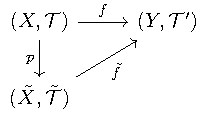
\includegraphics[]{otros/diagrama.pdf}
    \end{center}
    Además, \(f : (X, \T) \to (Y, \T)\) es una identificación si y solo si \(\tilde{f} : (\tilde{X}, \tilde{\T}) \to (Y, \T')\) es un homeomorfismo.
}
\pf{
    Si pretendemos que el diagrama sea conmutativo debe cumplirse
    \[
    \tilde{f}(p(x))=f(x)\iff \tilde{f}([x])=f(x)
    \]
    por tanto definimos $\tilde{f}$ de la siguiente manera:
    \[
    \tilde{f}:(\tilde{X}, \tilde{\T}) \to (Y, \T'),\quad \tilde{f}([x])=f(x).
    \]
    Ahora solo necesitamos ver que la aplicación está bien definida. En efecto si $x,y\in X$ son dos representantes de la misma clase de equivalencia $[x]$ entonces $xR_fy$, por tanto se cumple $f(x)=f(y)$, luego
    \[
    \tilde{f}([x])=f(x)=f(y)=\tilde{f}([y])
    \]
    por lo que la aplicación está bien definida\footnote{Está bien definida ya que hemos visto que la imagen de una clase de equivalencia no depende del representante escogido.}.

    Para la segunda parte, si suponemos que $\tilde{f}$ es un homeomorfismo entonces $f=\tilde{f}\circ p$ es continua por ser composición de funciones continuas, y es sobreyectiva por serlo $\tilde{f}$ y $p$. Además, si $U\in\T(f)$ entonces $f^{-1}(U)=p^{-1}(\tilde{f}^{-1}(U))\in\T$, por tanto $\tilde{f}^{-1}(U)\in\tilde{\T}$, y al ser $\tilde{f}$ abierta y biyectiva  $U=\tilde{f}(\tilde{f}^{-1}(U))\in\T'$, lo que prueba que $\T(f)=\T'$ y por tanto $f$ es una identificación.

    Si por el contrario suponemos que $f$ es una identificación entonces $f$ es sobreyectiva y $\T'=\T(f)$, por tanto $f$ es continua y al ser $p$ identificación también lo es $\tilde{f}$ (apartado 2 de la Proposición \hyperref[prop:114]{1.1.4}). Que $\tilde{f}$ es inyectiva es inmediato por  la propia definición de $\tilde{f}$. Para ver que es sobreyectiva, dado $y\in Y$ por ser $f$ sobreyectiva existe $x\in X\mid f(x)=y$, por tanto $\exists z=[x]\in\tilde{X}$ tal que $\tilde{f}([x])=f(x)=y$. Veamos que $\tilde{f}$ es abierta: dado $U\in\tilde{\T}$ entonces $f^{-1}(\tilde{f}(U))=p^{-1}(\tilde{f}^{-1}(\tilde{f}(U)))=p^{-1}(U)\in\T$ por ser $p$ continua, por lo tanto $\tilde{f}(U)\in\T(f)=\T'$, luego $\tilde{f}$ es un homeomorfismo.
}

\clearpage

\section{Ejemplos de espacios cocientes}

Veamos ahora algunos ejemplos de espacios cociente y la posibilidad de establecer homeomorfismos entre estos espacios cociente y otros espacios topológicos de interés. En estos primeros ejemplos haremos uso del Teorema \ref{thm:diagrama} para encontrar tales homeomorfismos.

\ex{
    Para el intervalo \(I = [0, 1]\), consideramos la partición:
    \[
    \tilde{I} = \{ \{0, 1\} \} \cup \{ \{x\} : x \in (0, 1) \}.
    \]
    El espacio cociente \((\tilde{I}, \tilde{\T})\) es homeomorfo a la circunferencia unidad \( \sphere^1 \).
}
\pf{
    Probemos que la relación $\sim$ dada por la partición $\tilde{I}$ coincide con la relación dada por la aplicación $f:I\to\sphere^1, f(t)=(\cos(2\pi t),\sin(2\pi t))$. Para ello, dados $x,y\in I$
    \[
    x R_f y \iff f(x)=f(y) \iff
    \begin{cases}
    \cos(2\pi x)=\cos(2\pi y)\\
    \sin(2\pi x)=\sin(2\pi y)
    \end{cases}
    \]
    Para que se den estas igualdades entre cosenos y senos hay varias opciones: si $x,y\in(0,1)$ entonces debe cumplirse $x=y$; si $x,y\in\{0,1\}$ entonces o bien $x=y$, o bien $x=0,y=1$, o bien $x=1,y=0$. En resumen:
    \[
    x R_f y \iff x=y \text{  o  } x=1,y=0 \text{  o  } x=0,y=1\iff x\sim y 
    \]
    Por tanto ambas son la misma relación. Ahora veamos que $f$ es una identificación, y por tanto $\exists \tilde{f}$ homeomorfismo entre $\tilde{I}$ y $\sphere^1$.

    En primer lugar, $f$ es continua por ser restricción de una aplicación continua (basta considerarla como aplicación de $I$ a $\R^2$), además es cerrada puesto que $I$ es compacto y $\sphere^2$ es Hausdorff (Ver Ejercicio \hyperref[exer:12]{1.2}). Por último dado $(x,y)\in\sphere^1$, denotemos por $\alpha=\text{ang}((x,y))$ al ángulo en radianes que forma el punto $(x,y)$ con la horizontal, con $\alpha\in[0,2\pi)$. Es sencillo comprobar que $f(\frac{\alpha}{2\pi})=(x,y)$, por tanto $f$ es sobreyectiva, lo que según la Proposición \hyperref[prop:114]{1.1.4} apartado 3 garantiza que $f$ es una identificación, y por tanto $\exists \tilde{f}$ homeomorfismo entre $\tilde{I}$ y $\sphere^1$
}

\exer{Probar que si $X$ es compacto, $Y$ es Hausdorff y $f:(X,\T)\to(Y,\T')$ es continua entonces $f$ es cerrada.}\label{exer:12}


\ex{
    Sea \(X = [0, 1] \times [0, 1]\) con la relación de equivalencia:
    \[
    (x_1, y_1) \sim (x_2, y_2) \text{ si y solo si } x_1 - x_2 \in \mathbb{Z} \text{ e } y_1 = y_2.
    \]
    El espacio cociente es homeomorfo a un cilindro.
}

\pf{
    Consideremos el cilindro $C=\{(x,y,z)\in\R^3 \mid x^2+y^2=1, z\in[0,1]\}$, probaremos que la relación $\sim$ coincide con la relación dada por la aplicación $f:X\to C, f(t,s)=(\cos(2\pi t),\sin(2\pi t),s)$. Para ello, dados $(x_1,y_1),(x_2,y_2)\in X$
    \[
        (x_1,x_2) R_f (x_2,y_2) \iff
        \begin{cases}
        \cos(2\pi x_1)=\cos(2\pi x_2)\\
        \sin(2\pi x_1)=\sin(2\pi x_2)\\
        y_1=y_2
        \end{cases}
    \]
    Dejamos como un sencillo ejercicio comprobar que para que se den estas igualdades entre cosenos y senos debe darse $x_1-x_2\in\mathbb{Z}$. En resumen:
    \[
        (x_1,x_2) R_f (x_2,y_2) \iff (x_1,y_1)\sim(x_2,y_2)
    \]
    Por tanto ambas son la misma relación. Ahora veamos que $f$ es una identificación, y por tanto $\exists \tilde{f}$ homeomorfismo entre $\tilde{X}$ y $C$.

    En primer lugar, $f$ es continua y cerrada por un argumento similar al del ejemplo anterior. Para ver que es sobreyectiva basta tomar $p=(x,y,z)\in C$, y denotemos por $\alpha=\text{ang}((x,y))$ al ángulo en radianes que forma el punto $(x,y)$ con la horizontal si consideramos a $(x,y)$ como punto de $\sphere^1$, con $\alpha\in[0,2\pi)$. Entonces $f(\frac{\alpha}{2\pi},z)=(x,y,z)=p$, por lo que $f$ es sobreyectiva y por tanto identificación.
}

\clearpage
\ex{
    Sea \(X = [0, 1] \times [0, 1]\) con la relación de equivalencia:
    \[
    (x_1, y_1) \sim (x_2, y_2) \text{ si y solo si } (x_1, y_1) = (x_2, y_2) \text{ o } [x_1 - x_2 = \pm 1 \text{ e } y_1 = 1 - y_2].
    \]
    El espacio cociente es homeomorfo a una banda de Möbius.
}

\pf{
    Llamamemos $M$ a la banda de Möbius. $M$ será la imagen de la función 
    \begin{gather*}
        F:[0,2\pi]\times[-1,1]\to\R^3 \\
        F(u,v)=((2-v\sin(\frac{u}{2}))\sin(u),(2-v\sin(\frac{u}{2}))\cos(u),v\cos(\frac{u}{2}))
    \end{gather*}
    es decir, $M=F([0,2\pi]\times[-1,1])$.

    Probaremos ahora que la función $f:I\times I\to M$ dada por $f(t,s)=F(2\pi t,2s-1)$ define la misma relación que $\sim$ y además es una identificación. La aplicación f es claramente continua, cerrada por ir de un compacto a un $T_2$ y sobreyectiva por definición (ya que $M=F([0,2\pi]\times[-1,1])=f(I\times I))$.
    
    En cuanto a la relación, dados $(x,y),(a,b)\in I\times I$
    \begin{gather*}
        (x_1,y_1)R_f(x_2,y_2) \iff f(x_1,y_1)=f(x_2,y_2) \iff\\
        \iff \begin{cases}
            (2-(2y_1-1)\sin(\pi x_1))\sin(2\pi x_1) =  (2-(2y_2-1)\sin(\pi x_2))\sin(2\pi x_2)\\
            (2-(2y_1-1)\sin(\pi x_1))\cos(2\pi x_1) = (2-(2y_2-1)\sin(\pi x_2))\cos(2\pi x_2) \\
            (2y_1-1)\cos(\pi x_1) = (2y_2-1)\cos(\pi x_2)
        \end{cases}
    \end{gather*}
    claramente si $(x_1, y_1) = (x_2, y_2) \text{ o } [x_1 - x_2 = \pm 1 \text{ e } y_1 = 1 - y_2]$ entonces se dan las igualdades y $(x_1,y_1)R_f(x_2,y_2)$. Por el contrario, si $(x_1,y_1)R_f(x_2,y_2)$ dejamos la comprobación de que debe cumplirse $(x_1, y_1) = (x_2, y_2) \text{ o } [x_1 - x_2 = \pm 1 \text{ e } y_1 = 1 - y_2]$ como ejercicio (o castigo) al lector.
}

\clearpage
\ex{
    Sea \(X = [0, 1] \times [0, 1]\) con la relación de equivalencia:
    \[
    (x_1, y_1) \sim (x_2, y_2) \text{ si y solo si } x_1 - x_2 \in \mathbb{Z} \text{ e } y_1 - y_2 \in \mathbb{Z}.
    \]
    El espacio cociente es homeomorfo a un toro.
}

\pf{
    En primer lugar notemos que la relación de equivalencia consiste en identificar los lados del cuadrado $[0, 1] \times [0, 1]$ según la siguiente figura
    \begin{center}
        \includegraphics[width=0.2\textwidth]{img/cociente-toro.png}
    \end{center}
    En cuanto al toro $\mathbb{T}$, lo consideraremos como el subconjunto de $\R^3$ de la siguiente forma
    \[
    \mathbb{T}=\{(x,y,z)\in\R^3 \mid (\sqrt{x^2+y^2}-2)^2+z^2=1\}
    \]
    Si definimos la función
    \begin{gather*}
        F:[0,2\pi]\times[0,2\pi]\to\mathbb{T} \\
        F(u,v)=(\cos u(\cos v+2),\sin u(\cos v+2),\sin v)
    \end{gather*}
    basta comprobar que
    \[
    f:[0,1]\times[0,1]\to \mathbb{T},\quad f(t,s)=F(2\pi t,2\pi s)
    \]
    induce la misma relación de equivalencia que $\sim$, y además es continua, sobreyectiva y cerrada (por ir de un compacto a un Hausdorff). Todas estas comprobaciones, muy similares a las de los anteriores ejemplos, quedan como un sencillo ejercicio para el lector.
}

\clearpage

\ex{
    Sea \(X = [0, 1] \times [0, 1]\) con la relación de equivalencia:
    \[
    (x_1, y_1) \sim (x_2, y_2) \text{ si y solo si } [x_1 = x_2 \text{ e } y_1 - y_2 \in \mathbb{Z}] \text{ o } [x_1 - x_2 = \pm 1 \text{ e } y_1 = 1 - y_2].
    \]
    El espacio cociente es homeomorfo a una botella de Klein.
}

\pf{
    Definiremos la botella de Klein $K$ como el subconjunto de $\R^4$ dado por la imagen de la siguiente función:
    \begin{gather*}
        f:[0,1]\times[0,1]\to K\subset \R^4 \\
        f(t,s)=
        ((2+\cos(2\pi t))\cos(2\pi s),\\
        (2+\cos(2\pi t))\sin(2\pi s),\\
        \sin(2\pi t)\cos(\pi s),\\
        \sin(2\pi t)\sin(\pi s))
    \end{gather*}
    Claramente $f$ es continua, sobreyectiva (por la propia definición de $K$) y cerrada (por ir de un compacto a un $T2$). Además, se puede comprobar que determina la misma relación de equivalencia que $\sim$, por lo que en virtud de la Proposición 4.1 existe un homeomorfismo entre $\tilde{X}$ y la botella de Klein.
}

\clearpage

\ex{
    Sea \(X = \mathbb{S}^1 \times [0, 1]\) con la relación de equivalencia:
    \[
    (x_1, y_1) \sim (x_2, y_2) \text{ si y solo si } y_1 = y_2 = 0 \text{ o } (x_1, y_1) = (x_2, y_2).
    \]
    El espacio cociente es homeomorfo a un cono.
}

\pf{
    Definamos el cono
    \[
    C=\{(x,y,z)\in\R^3\mid x^2+y^2=z^2,z\in[0,1]\}
    \]
    y tomemos la función
    \begin{gather*}
        f:\sphere^1\times[0,1]\to C\\
        f(\theta,t)=(t\theta_x,t\theta_y,t),\quad \theta=(\theta_x,\theta_y)\in\sphere^1\subset\R^2
    \end{gather*}
    es inmediato ver que la función es continua, sobreyectiva y cerrada por argumentos como los del resto de ejemplos. Por otro lado
    \[
    (\theta,t)R_f(\theta',t')\iff t=t', t\theta=t'\theta' \iff t=t'=0\quad \text{ó} \quad (\theta,t)=(\theta',t')\iff (\theta,t)\sim(\theta',t')
    \]
    Por tanto existe un homeomorfismo entre $C$ y $\tilde{X}$.
}

\clearpage

\ex{
    Sea \(X = \mathbb{S}^2\) con la relación de equivalencia:
    \[
    p \sim q \iff p = \pm q.
    \]
    El espacio cociente $\tilde{\mathbb{S}}^2$ es homeomorfo al plano proyectivo \(\mathbb{RP}^2\).
}

\pf{
    En primer lugar, el plano proyectivo $\mathbb{RP}^2$ será el conjunto cociente obtenido al considerar la siguiente relación $\sim_p$ sobre $\R^3\setminus\{0\}$. 
    \[
    x \sim_p y\iff x=\lambda y, \lambda\neq 0.
    \]
    La idea va a ser construir una aplicación de $\R^3\setminus\{0\}$ a $\mathbb{S}^2$ de tal manera que la aplicación respeta la relación que existe sobre $\mathbb{S}^2$, es decir, $x\sim_p y\iff f(x)\sim f(y)$. Similarmente, veremos que existe una aplicación de $\mathbb{S}^2$ a $\R^3\setminus\{0\}$ que también respeta la relación de equivalencia del proyectivo. Esto garantiza que las aplicaciones "pasan al cociente". Finalmente veremos que estas aplicaciones en el cociente son homeomorfismos y que la una es la inversa de la otra. La idea se resume en el siguiente diagrama, donde $\pi_1,\pi_2$ son las proyecciones a los cocientes.
    \begin{center}
        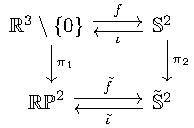
\includegraphics[width=0.25\textwidth]{otros/diagrama-proyectivo-esfera.pdf}
    \end{center}

    Definamos $f:\R^3\setminus\{0\}\to\sphere^2$ por $f(x)=\frac{x}{|x|}$, y $\iota:\sphere^2\to\R^3\setminus\{0\}$ por $\iota(x)=x$. Notemos que si $x,y\in\R^3\setminus\{0\}$ están relacionados entonces:
    \[
    x\sim_p y\iff x=\lambda y,\lambda\neq 0 
    \]
    y por tanto
    \[
    f(x)=\frac{x}{|x|}=\frac{\lambda y}{|\lambda||y|}=\pm\frac{y}{|y|}=\pm f(y) \iff f(x)\sim f(y).
    \]
    Además, si $f(x)\sim f(y)$ entonces 
    \[
    \frac{x}{|x|}=\pm\frac{y}{|y|}\implies x=\lambda y, \lambda \ne 0
    \]
    en esencia hemos visto que $x\sim_p y\iff f(x)\sim f(y)$, lo que garantiza que la aplicación $\tilde{f}([x]_p)=[f(x)]$\footnote{Usamos $[\cdot]_p$ para referirnos a las clases de equivalencia en el proyectivo y $[\cdot]$ para las clases de equivalencia en $\sphere^2$.} está bien definida puesto que
    \[
        \tilde{f}([x]_p)=\tilde{f}([y]_p)\iff [f(x)]=[f(y)]\iff f(x)\sim f(y) \iff x\sim_p y\iff [x]_p=[y]_p.
    \]
    
    La demostración de que $\iota$ también pasa al cociente se deja como un sencillo ejercicio. Veamos ahora que $\tilde{f}$ y $\tilde{\iota}$ son inversas la una de la otra
    \[
    \tilde{f}(\tilde{\iota}([x]))=\tilde{f}([x]_p)=[f(x)]=\left[\frac{x}{|x|}\right]=[x]
    \]
    donde la última igualdad se sigue de que $x\in\sphere^2$ y por tanto $|x|=1$. Por otro lado
    \[
    \tilde{\iota}(\tilde{f}([x]_p))=\tilde{\iota}([f(x)])=\tilde{\iota}(\left[\frac{x}{|x|}\right])=\left[\frac{x}{|x|}\right]_p=[x]_p
    \]
    donde la última igualdad se sigue del hecho de que $\frac{x}{|x|}\sim_p x$.

    Veamos ahora que 
}

\clearpage

\ex{
    En el disco cerrado \(D(0, 1)\) de \(\mathbb{R}^2\), consideramos la relación de equivalencia:
    \[
    (x_1, y_1) \sim (x_2, y_2) \text{ si y solo si } x_1 = \pm x_2 \text{ e } y_1 = y_2.
    \]
    El espacio cociente \(\faktor{D(0, 1)}{\sim}\) es homeomorfo a la esfera \(\mathbb{S}^2\).
}

\pf{
    Se deja como ejercicio.
}

\exer{
    Dado $(X,\T)$ un espacio topológico y $K\subset X$, definimos la relación
        \[
            x \sim y\iff
            \begin{cases}
                x,y \in K \\
                x=y
            \end{cases}
        \]
    y llamemos al espacio cociente $(\faktor{X}{K},\faktor{\T}{K}):=(\faktor{X}{\sim},\faktor{\T}{\sim})$.
        \begin{enumerate}
            \item[a)] Demostrar que $p|_{X\setminus K}:X\to p(X\setminus K)$ es una biyección.
            \item[b)] Demostrar que $p|_{X\setminus K}$ es un homeomorfismo si $K$ es abierto o cerrado.
        \end{enumerate}
}

\noindent\textbf{Solución:}

Para el apartado a) notemos que
\[
    \forall x \in X \setminus K,\quad p|_{X\setminus K}(x)=[x]
\]
pero por la manera en la que está definida la relación de equivalencia, es inmediato ver que $[x]=\{x\}$, ya que el único elemento relacionado con $x$ es el propio $x$ (recordemos que $x\notin K$). Por tanto $p|_{X\setminus K}$ es inyectiva ya que
\[
    p|_{X\setminus K}(x)=p|_{X\setminus K}(y)\implies [x]=[y]\implies \{x\}=\{y\}\implies x=y
\]
y además es sobreyectiva por estar definida en su imagen. Por tanto $p|_{X\setminus K}$ es una biyección.

Para el apartado b) notemos en primer lugar que $p$ es continua, por lo que $p|_{X\setminus K}$ también lo será por ser su restricción a $X\setminus K$.

Haremos el caso $K$ cerrado, cuando $K$ es abierto hay que razonar de manera idéntica pero con cerrados teniendo en cuenta la parte 3 de la Proposición \hyperref[prop:112]{1.1.2}.

Si  $K$ es cerrado entonces $X\setminus K$ es abierto, ahora si tomamos $U\in\T|_{X\setminus K}$ entonces $U=\tilde{U}\cap (X\setminus K), \tilde{U}\in\T$. Pero como $X\setminus K$ es abierto entonces de hecho $U\in\T$ y por tanto
\[
p^{-1}(p(U))=(p|_{X\setminus K})^{-1}(p|_{X\setminus K}(U))=U\in\T
\]
(recordemos que $p|_{X\setminus K}$ es una biyección y por tanto tiene inversa).
Finalmente por la definición de topología cociente debe de ser $p(U)\in\faktor{\T}{K}$, pero como además $p|_{X\setminus K}(U)=p(U)=p(U)\cap p(X\setminus K)$ deducimos que $p|_{X\setminus K}(U)\in\faktor{\T}{K}|_{p(X\setminus K)}$, lo que prueba que $p|_{X\setminus K}$ es abierta y por tanto un homeomorfismo.

\clearpage

\section{Espacios localmente euclídeos}

\defn{Espacio localmente euclídeo}{
    Un espacio topológico \((X, \T)\) se dice que es localmente euclídeo de dimensión \(n\) si todo punto \(p\) de \(X\) tiene un entorno \(U\) homeomorfo a una bola abierta \(B\) de \(\mathbb{R}^n\). Si \(\varphi: U \subset X \to B \subset \mathbb{R}^n\) es tal homeomorfismo, \((U, \varphi)\) se llama carta en \(X\) alrededor de \(p \in U\).
}

\rmkb{
    \begin{enumerate}
        \item Por ser \(X\) localmente euclídeo, este hereda las propiedades locales de \(\mathbb{R}^n\).
        \item Podemos sustituir la bola abierta en la definición anterior por un entorno abierto de \(\mathbb{R}^n\).
    \end{enumerate}
}

\defn{Bola euclídea}{
    Diremos que \(B' \subset X\) es una bola euclídea si $B'$ es homeomorfo a una bola abierta $B(0,r)$ de $\R^n$.
}

\defn{Bola regular euclídea}{
    Diremos que \(B \subset X\) es una bola regular euclídea si:
    \begin{itemize}
        \item Existe una bola euclídea \(B'\) tal que \(\overline{B} \subset B'\).
        \item Existe \(r > 0\) y una carta \(\varphi: B' \to B^n(0, 2r)\) tal que \(\varphi(\overline{B}) = \overline{B^n(0, r)}\).
    \end{itemize}
}

\section{Variedades topológicas}

\defn{Variedad topológica}{
    Una variedad topológica \(M\) es un espacio topológico \(T_2\) y \(2A\N\) que es localmente euclídeo. La dimensión de \(M\) es el número natural \(n\). También se denomina \(n\)-variedad (topológica).
}

\defn{Superficie topológica}{
    Una superficie topológica \(S\) es una variedad topológica de dimensión dos o 2-variedad.
}

\rmkb{
    En ocasiones podemos referirnos a las superficies topológicas como superficies, o en general a las $n$-variedades topológicas como $n$-variedades (o incluso variedades si se sobrentiende su dimensión). Cabe destacar que en otro contextos la palabra superficie puede referirse a un concepto distinto, como el de superficie parametrizada o el de variedad diferenciable de dimensión 2 (superficie regular).
}

\defn{Variedad con borde}{
    Si en la definición de variedad cambiamos el espacio modelo \(\mathbb{R}^n\) por el semiespacio superior \(\mathbb{H}^n = \{x \in \mathbb{R}^n : x_i \geq 0\}\), obtenemos el concepto de variedad con borde.
}

\propp{Observaciones sobre variedades topológicas}{
    \begin{enumerate}
    \item Toda variedad topológica es localmente conexa por caminos (y localmente conexa).
    \item Las componentes conexas y las componentes conexas por caminos coinciden en una variedad.
    \item Una variedad es conexa si y solo si es conexa por caminos.
    \item Toda variedad es localmente compacta.
    \item Si una variedad no es compacta, siempre podremos compactificarla añadiendo un solo punto.
    \end{enumerate}
}{
  Sea $M$ una n-variedad. Notemos en primer lugar la siguiente afirmación que usaremos para probar el punto 4:
  \clmp{}{
     Dado $x\in M$, como $M$ es una variedad existe un entorno $U\in\E(x)$ homeomorfo a una bola $B(0,r)=\varphi(U)$ de $\R^n$ con $\varphi(x)=0$.
  }{
    Sabemos por ser $M$ variedad que existe un entorno $U'\in\E(x)$ y un homeomorfismo 
    
    \noindent$\psi:U'\to B$ con $B$ una bola en $\R^n$. Si $\psi(x)=0$ ya hemos acabado, si $\psi(x)\neq 0$ entonces podemos elegir una bola centrada en $\psi(x)$ de radio $r'$ lo suficientemente pequeño de manera que $B(\psi(x),r')\subset B\implies A=\psi^{-1}(B(\psi(x),r'))\subset\psi^{-1}(B)=U$, y $A\in\E(x)$. Finalmente la aplicación $\phi:B(\psi(x),r')\to B(0,r'), \phi(s)=s-\psi(x)$ es un homeomorfismo, por lo que $\varphi=\phi\circ\psi|_{A}:A\to B(0,r')$ es el homeomorfismo buscado.
  }

  De hecho dado cualquier $V\in\E(x)$ siempre podemos elegir el entorno homeomorfo a una bola de manera que $U\subset V$ puesto que si $U\not\subset V$, entonces basta tomar $B'(0,r')\subset B(0,r)$ lo suficientemente pequeña para que $U'=\varphi^{-1}(B'(0,r'))\subset U\cap V$ y claramente $U'$ también es homeomorfo a una bola de $\R^n$.
    \begin{enumerate}
      \item Sean $x\in M, V\in\E(x)$, como $M$ es una variedad existe un entorno $U\in\E(x),U\subset V$ homeomorfo a una bola de $\R^n$, y por tanto localmente conexo por caminos. Como $U$ es localmente conexo por caminos $\exists U'\subset U$ un entorno de $x$ conexo por caminos. Por último notemos que $U'\subset U\subset V\implies U'\subset V$, luego $U'$ es un entorno de $x$ conexo por caminos contenido en $V$, lo que prueba que $M$ es localmente conexa por caminos. Que es localmente conexa es inmediato puesto que localmente conexo por caminos implica localmente conexo. 
      \item Se sigue de las propiedades generales de un espacio localmente conexo por caminos.
      \item Se sigue de las propiedades generales de un espacio localmente conexo por caminos.
      \item Sea $x\in M$, como $M$ es una variedad existe un entorno $U\in\E(x)$ homeomorfo a una bola $B(0,r)$ mediante un homeomorfismo $\varphi : B(0,r)\rightarrow U $ con $\varphi(0) = x$. Puesto que $\overline{B(0,\frac{r}{2})}$ es compacto y $\varphi$ es continua, $\varphi(\overline{B(0,\frac{r}{2})})$ es un compacto. Además $\varphi(\overline{B(0,\frac{r}{2})})\subset\varphi(B(0,r))=U$ por lo que si tomamos $C=\varphi(\overline{B(0,\frac{r}{2})})$ como compacto y $U$ como entorno se verifica que $x\in C\subset U$, por lo que $M$ es localmente compacta en $x$, como el punto elegido era arbitrario $M$ es localmente compacta.
      \item Como cualquier variedad es $T_2$ y locamente compacta el Teorema de Alexandroff nos asegura que podemos compactificarla por un punto.
    \end{enumerate}
}

\clearpage

\subsection{Ejemplos de superficies}

En todos los ejemplos siguientes consideramos subespacios de algún $\R^m$, por tanto todos los espacios son $T_2$ y $2A\N$ (recordemos que estas propiedades se heredan al considerar las topologías relativas). Solo necesitamos probar que cada uno de estos espacios son localmente euclídeos.

\ex{
  La esfera \(\mathbb{S}^2\) es una superficie topológica.
}

\noindent\textbf{Solución:}

  Sea $p=(x,y,z)\in\sphere^2$ y supongamos que $z>0$, en tal caso el entorno $U=\sphere^2\cap\{z>0\}$ es homeomorfo a la bola $B^2((0,0),1)$ mediante el homeomorfismo
  \[
  \varphi:B^2((0,0),1)\to U,\quad \varphi(x,y)=(x,y,\sqrt{x^2+y^2}).
  \]
  En efecto es una homeomorfismo pues es abierta, continua y biyectiva, con inversa
  \[
  \varphi^{-1}(x,y,z)=(x,y).
  \]
  Para el resto de puntos sabemos que alguna de las tres componentes $x,y,z$ debe ser no nula, por lo que podemos hacer un procedimiento similar, tarea que encomendamos al lector.



\ex{
    El toro \(\mathbb{T}^2 = \mathbb{S}^1 \times \mathbb{S}^1\) es una superficie topológica.
}

\ex{
    El cilindro \(\mathbb{S}^1 \times \mathbb{R}\) es una superficie topológica.
}

\ex{
    El hiperboloide de una hoja \(x^2 + y^2 - z^2 = 1\) es una superficie topológica.
}

\ex{
    El hiperboloide de dos hojas \(x^2 + y^2 - z^2 = -1\) es una superficie topológica.
}

\ex{
    El paraboloide de revolución \(x^2 + y^2 - z = 0\) es una superficie topológica.
}

\clearpage % Para que quede toda la proposición en la misma página

\propp{Espacio proyectivo real}{
    El espacio proyectivo real \(\mathbb{RP}^n\) es una variedad topológica de dimensión \(n\).
}{
    Veamos en primer lugar qué tipo de espacio topológico es $\mathbb{RP}^n$. Para ello, notemos que está definido por la relación de equivalencia sobre $\R^{n+1}\setminus\{0\}$ dada por
    \[
    x \sim y \iff x=\lambda y, \lambda\neq 0.
    \]
    Podemos dar una expresión explicita de las clases de equivalencia en $\mathbb{RP}^n$ como
    \[
        [x_1,\cdots,x_{n+1}]=\{(\lambda x_1,\cdots,\lambda x_{n+1}):\lambda\in\R\setminus\{0\},\exists x_{i_0}\neq 0\}
    \]
    en cuyo caso la proyección al cociente viene dada por
    \[
    \pi:\R^{n+1}\setminus\{0\}\to\mathbb{RP}^n,\quad \pi(x_1,\dots x_{n+1})=[x_1,\dots,x_{n+1}]
    \]
    Veamos que $\mathbb{RP}^n$ es localmente euclídeo. Sea $p=[x_1,\cdots,x_{n+1}]\in\mathbb{RP}^n$, por definición de $\mathbb{RP}^n$ sabemos que existe un $i_0$ tal que $x_{i_0} \neq 0$, definimos el siguiente entorno $U_p = \{[y_1,\cdots,y_{n+1}] : y_{i_0} \neq 0 \}$ que contiene a $p$ y es abierto puesto que la topología sobre $\mathbb{RP}^n$ es precisamente la topología final de $\pi$ y se tiene $\pi^{-1}(U_p)=V_p$ donde
    \[
        V_p=\{(y_1,\cdots,y_{n+1}) : y_{i_0} \neq 0\}
    \]
    que es abierto puesto que su complementario
    \[
        \left[\R^{n+1}\setminus\{0\}\right]\setminus V_p=\{(y_1,\cdots,y_{n+1}) : y_{i_0} = 0\}
    \]
    es cerrado. Por tanto $U_p$ es abierto (recuérdese la definición de topología final), y la siguiente aplicación
    \[
    \varphi :U_p \to \mathbb{R}^n,\quad \varphi([x_1,\cdots,x_{n+1}])=\left(\frac{x_1}{x_{i_0}},\cdots,\frac{x_{i_0-1}}{x_{i_0}},\frac{x_{i_0+1}}{x_{i_0}},\cdots,\frac{x_{n+1}}{x_{i_0}}\right)
    \]
    es un homeomorfismo. Omitiremos ver que $\varphi$ esta bien definida y es un homeomorfismo.

    %TODO Justificar que es Hausdorff y 2AN.
}

\clearpage

\subsection{Propiedades de las variedades topológicas}

Comenzamos demostrando sin demasiado detalle un pequeño lema técnico.

\lem{Lema técnico}{
    Sea $B=B(0,1)\subset\R^n$ la bola abierta de centro $0$ y radio $1$ y sean $p,q\in B$. Entonces existe un homeomorfismo $\phi:\overline{B}\to\overline{B}$ de manera que $\phi(p)=q$ y $\phi|_{\partial B}=Id.$
}
\pf{
    Sea $\mu:B\to\R^n,\mu(x)=\frac{x}{1-|x|}$, es fácil comprobar que $\mu$ es un homeomorfismo. Definamos la aplicación $\phi:\overline{B}\to\overline{B}$ por
    \[
    \phi(x) =
    \begin{cases}
        \mu^{-1} \bigl( \mu(x) - \mu(p) + \mu(q) \bigr), & x \in B \\
        x, & x \in \partial B
    \end{cases}
    \]
    se puede comprobar que $\phi$ es continua en la frontera de $B$ y que también lo es su inversa, por tanto es un homeomorfismo que cumple $\phi(p)=q,\phi|_{\partial B}=Id$.
}

\thmr{Proposición 4.2 - Homogeneidad}{homogeneidad}{
    Sea \(X\) una variedad topológica conexa de dimensión \(n\) y \(p\), \(q \in X\). Entonces existe un homeomorfismo \(f : X \to X\) tal que \(f(p) = q\).
}
\pf{
    Sea la relación de equivalencia en $X$ dada por 
    \[
    p \sim q\iff
    \exists f : X \to X \text{ homeomorfismo tal que } f(p) = q.
    \]
    Vamos a ver que $[p]$ es abierta y cerrada en $X$, y, por tanto, es todo $X$ al ser $X$ conexo.

    Para ver que es abierta sea $q\in[p]$, veremos que podemos encontrar un entorno de $q$ contenido en $[p]$. Por ser $X$ localmente euclídeo existe $U\in\E(q)$ homeomorfo a una bola de $\R^n$. Como todas las bolas son homeomorfas podemos elegir un homeomorfismo de la siguiente forma
    \[
    \varphi:B^n(0,2)\to U,\quad \varphi(0)=q,\quad 0=\varphi^{-1}(q).
    \]
    Consideremos ahora los conjuntos $B=B^n(0,1), B'=\varphi(B)$. Notemos que ambos son abiertos en sus respectivas topologías. Definamos ahora la aplicación
    \[
    \tilde{\varphi}:\overline{B}\to\overline{B'},\quad \tilde{\varphi}(x)=\varphi(x)
    \]
    y veamos que es un homeomorfismo. En efecto por ser $\varphi$ continua y cerrada se tiene
    \[
    \varphi(\overline{B})\subset\overline{\varphi(B)}=\overline{B'}\subset\overline{\varphi({\overline{B}})}=\varphi(\overline{B})\implies \varphi(\overline{B})=\overline{B'}
    \]
    por lo que $\tilde{\varphi}$ está bien definida y es sobreyectiva. Finalmente notemos que $\tilde{\varphi}$ es la restricción de un homeomorfismo y es sobreyectiva, y por tanto es un homeomorfismo. Démonos cuenta también de que
    \[
        \tilde{\varphi}(\partial B)=\tilde{\varphi}(\overline{B}\setminus B)=\tilde{\varphi}(\overline{B})\setminus \tilde{\varphi}(B)=\overline{B'}\setminus B'=\partial B'
    \]

    Veamos ahora que $B'\subset[p]$, para ello sea $y\in B'$, de manera que $y=\varphi(x), x\in B$. Por el lema anterior, como $0,x\in B$ existe un homeomorfismo $\phi:\overline{B}\to\overline{B}$ de manera que $\phi(0)=x$ y $\phi|_{\partial B}=Id.$
    Definamos ahora la siguiente aplicación
    \[
    F:\overline{B'}\to\overline{B'},\quad F=\tilde{\varphi}\circ\phi\circ\tilde{\varphi}^{-1}
    \]
    que es un homeomorfismo por ser composición de homeomorfismos y además cumple
    \[
    F(q)=\tilde{\varphi}(\phi(\tilde{\varphi}^{-1}(q)))=\tilde{\varphi}(\phi({\varphi}^{-1}(q)))=\tilde{\varphi}(\phi(0))=\tilde{\varphi}(x)=\varphi(x)=y
    \]
    Si tomamos $z\in{\partial B'}$ entonces $\tilde{\varphi}^{-1}(z)\in \partial B$, por lo que $\phi(\tilde{\varphi}^{-1}(z))=\tilde{\varphi}^{-1}(z)$ luego
    \[
    F(z)=\tilde{\varphi}(\phi(\tilde{\varphi}^{-1}(z)))=\tilde{\varphi}(\tilde{\varphi}^{-1}(z))=z \implies F|_{\partial B'}=Id.
    \]
    Ahora, por el lema del pegado para aplicaciones continuas la aplicación
    \[
    f:X\to X,\quad f(x)=
    \begin{cases}
        F(x), & x \in \overline{B'} \\
        x, & x \in X\setminus B'
    \end{cases}
    \]
    es continua ya que $\overline{B'},X\setminus B'$ son cerrados y tanto $F$ como $Id$ son continuas en cada uno de estos respectivos cerrados, coincidiendo además sus valores en la intersección $\partial B'$. Por un argumento completamente análogo podemos ver que la inversa de $f$
    \[
    f^{-1}:X\to X,\quad f^{-1}(x)=
    \begin{cases}
        F^{-1}(x), & x \in \overline{B'} \\
        x, & x \in X\setminus B'
    \end{cases}
    \]
    es también continua, lo que prueba que $f$ es un homeomorfismo en $X$ que además satisface $f(q)=F(q)=y$, por tanto $\forall y\in B'$ se tiene $y\sim q\sim p\implies y\sim p$, lo cual quiere decir que $B'\subset [p]$, luego $[p]$ es abierto.

    Hemos visto que $[p]$ es abierto. Además, $X\setminus[p] = \bigcup_{q \ne p} [q]$, porque las clases de equivalencia son disjuntas. Al ser unión arbitraria de abiertos es abierto, luego el complementario $[p]$ es cerrado. Como $X$ es conexo y $[p]$ es abierto y cerrado debe ser $[p]=X$, lo que finaliza la demostración.
}

\clearpage

\section{Unión disjunta}

\defn{Unión disjunta}{
    Sea \(\{(X_\alpha, \T_\alpha)\}_{\alpha \in J}\) una familia indexada de espacios topológicos. Definimos su unión disjunta como:
    \[
    \bigsqcup_{\alpha \in J} X_\alpha = \{(x, \alpha) : x \in X_\alpha, \alpha \in J\}.
    \]
    Consideramos las inyecciones canónicas \(\iota_\alpha : X_\alpha \to \bigsqcup_{\alpha \in J} X_\alpha\), dadas por \(\iota_\alpha(x) = (x, \alpha)\).
}

\rmkb{
    Para entender la unión disjunta podemos pensar en ek siguiente contexto. Supongamos que los espacios topológicos son subconjuntos acotados del plano (por ejemplo polígonos), su unión disjunta consistirá en disponer estos subconjuntos de tal manera que no se solapen unos con otros. Un ejemplo sería la imagen siguiente
    \begin{center}
        \includegraphics[width=0.25\textwidth]{img/union-disjunta.png}
    \end{center}
    Otra manera de imaginar la unión disjunta es considerar que ponemos cada subconjunto del plano en una copia distinta de $\R^2$, es decir, tendremos cada espacio topológico (figura) en un plano y la unión disjunta será la unión de esas "hojas".
}

\propp{Topología unión disjunta}{
    La familia de subconjuntos \(B = \{\iota_\alpha(U) : U \in \T_\alpha, \alpha \in J\}\) es una base para una topología \(\T\) sobre \(\bigsqcup_{\alpha \in J} X_\alpha\) que recibe el nombre de topología unión disjunta.
}{
    Sea \(\{(X_\alpha,\T_\alpha)\}_{\alpha\in J}\) una familia de espacios topológicos.
    \newline
    (B1) Para todo \((x,\alpha)\in\bigsqcup_{\alpha\in J}X_\alpha\) se tiene $x\in X_\alpha$, y como $X_\alpha\in \T_\alpha$, deducimos que $(x,\alpha) \in \iota_\alpha(X_\alpha)\in B$.
    \newline
    (B2) Si \((x,\alpha)\in\iota_\alpha(U_1)\cap\iota_\beta(U_2)\) necesariamente  $\alpha = \beta$ puesto que en otro caso
    \[
        \iota_\alpha(U_1)\cap\iota_\beta(U_2) = \emptyset
    \]
    que es una contradiccion con que $x$ esta en la intersección. Entonces \(x\in U_1\cap U_2\) y existe \(V=U_1\cap U_2\in \T_\alpha\) (que es abierto puesto que $U_1,U_2$ lo son) con \(x\in V\subset U_1\cap U_2\), por lo que \((x,\alpha)\in\iota_\alpha(V)\subset\iota_\alpha(U_1)\cap\iota_\beta(U_2)\). La última inclusión es fácil de comprobar y se deja como un sencillo ejercicio.
}

\propp{Propiedades de la unión disjunta}{
    \begin{enumerate}
        \item Cada inclusión \(\iota_{\alpha}\) es un embebimiento, por lo que podemos identificar 
        
        \(X_{\alpha} \equiv \iota_{\alpha}(X_{\alpha}) \subset \bigsqcup_{\alpha \in J} X_{\alpha}\).  
        \item Un subconjunto es abierto en \(\bigsqcup_{\alpha \in J} X_{\alpha}\) si y solo si su intersección con cada \(X_{\alpha}\) es un abierto en \(X_{\alpha}\).  
        \item Una aplicación \(f : \bigsqcup_{\alpha \in J} X_{\alpha} \to Y\) es continua si y solo si \(f|_{X_{\alpha}}\) es continua, para todo \(\alpha \in J\).  
        \item Si todos los espacios \(X_{\alpha}\) son \(T_2\) (resp. \(1A\N\)), la unión disjunta también es \(T_2\) (resp. \(1A\N\)).  
        \item Si todos los espacios \(X_{\alpha}\) son \(2A\N\) y \(J\) es numerable, entonces la unión disjunta también es \(2A\N\).  
        \item La unión disjunta de una cantidad numerable de \(n\)-variedades es una \(n\)-variedad.
    \end{enumerate}
}{
    Pendiente.
}

\clearpage

\section{Suma conexa}

\defn{Suma conexa}{
    Sean \(S_1\) y \(S_2\) dos superficies conexas y sean \(D_1\) y \(D_2\) discos regulares euclídeos. Sea \(\varphi : \partial D_1 \to \partial D_2\) un homeomorfismo y denotemos por \(S_i' := S_i \setminus D_i, \ i = 1, 2\). Definimos en \(S_1' \sqcup S_2'\) la menor relación de equivalencia que contiene a \(x \sim \varphi(x)\) para todo \(x \in \partial D_1\). Entonces el cociente \(\faktor{S_1' \sqcup S_2'}{\sim}\) es un espacio topológico.
}

\rmkb{El homeomorfismo $\varphi : \partial D_1 \to \partial D_2$ existe siempre puesto que las fronteras de los discos son homeomorfas a las fronteras de alguna bola euclídea, y por tanto ambas fronteras son homeomorfas a la circunferencia unidad
\[
    \partial D_1\cong \sphere^1\cong\partial D_2.
\]
}

A continuación se enuncian un par de lemas que serán útiles para la demostración de la Proposición \hyperref[prop:invarianza-cociente]{1.7.4}. El primero es una generalización del conocido Teorema de la Curva de Jordan, el cual se enuncia sin demostración. El segundo es un lema técnico, que sí demostraremos.

\lem{Teorema de Jordan - Schönflies}
{
    \label{lem:jordan}
    Sean $C$ y $C'$ dos curvas cerradas simples de $\mathbb{R}^2$, y $f : C \to C'$ un homeomorfismo. Entonces existe un homeomorfismo $F : \mathbb{R}^2 \to \mathbb{R}^2$ tal que $F\vert_C = f$ y fuera de un compacto $K \supseteq C$ es la identidad.
}

\lemp{Extensión de homeomorfismos de $\mathbb{S}^1$}{\label{lem:extension-homeo}
    Sean $C_1, C_2$ homeomorfos a $\mathbb{S}^1$, $h: C_1 \to C_2$ un homeomorfismo y $U \subseteq \mathbb{R}^2$ abierto, $U\cong \mathbb{R}^2$, con $C_1 \cup C_2 \subseteq U$. Entonces existe un homeomorfismo $H : \mathbb{R}^2 \to \mathbb{R}^2$ tal que $H\vert_{C_1} = h$ y $H\vert_{\mathbb{R}^2 \setminus U} = Id$.
}{
    Sea $g:U\to\mathbb{R}^2$ el homeomorfismo dado por la hipótesis $U\cong\R^2$ y sean $\tilde{C}_1 = g(C_1),\tilde{C}_2 = g(C_2)$, definamos la aplicación
    \[
        \hat{h} = \left(g\circ h\circ g^{-1}\right)|_{\tilde{C}_1} : \tilde{C}_1 \to \tilde{C}_2.
    \]
    que es claramente un homeomorfismo. Por el Teorema de Jordan-Schönflies existe un homeomorfismo $\hat{H}:\mathbb{R}^2\to\mathbb{R}^2$ tal que $\hat{H}\vert_{\tilde{C}_1} = \hat{h}$ y $\hat{H}$ es la identidad fuera de un compacto $K\supseteq\tilde{C}_1$. Sea $H = g^{-1}\circ\hat{H}\circ g$, entonces $H$ es el homeomorfismo buscado puesto que para todo $x\in C_1$
    \begin{align*}
    H|_{C_1}(x) &= \left(g^{-1}\circ \hat{H} \circ g \right)|_{C_1}(x)=\left(g^{-1}\circ \hat{H}|_{\tilde{C}_1}\right)(g(x))=\left(g^{-1}\circ\hat{h}\right)(g(x))=
    \\
    &= \left(g^{-1}\circ g\circ h\circ g^{-1}\right)(g(x))=h(x)\implies H|_{C_1}=h
    \end{align*}
    Además, si $K\subset U$ entonces claramente $H\vert_{\mathbb{R}^2 \setminus U} = Id$, y siempre podemos suponer que $K\subset U$ porque $U$ es homeomorfo a $\R^2$. % Que alguien revise esto porque no estoy muy seguro la verdad
}

\propp{Invarianza del cociente \(\faktor{S_1' \sqcup S_2'}{\sim}\)}{\label{prop:invarianza-cociente}
    Si \(S_1\) y \(S_2\) son dos superficies topológicas conexas, entonces, salvo homeomorfismo, el espacio \(\faktor{S_1' \sqcup S_2'}{\sim}\) no depende de los discos regulares euclídeos ni del homeomorfismo \(\varphi\).
}{
    Veremos la demostración en 3 pasos:

    \begin{enumerate}
        \item \textbf{El tamaño del disco no importa.}

        Sean $D_1$ y $D_3$ discos regulares y euclídeos centrados en $p\in S_1$, y supongamos que $\overline{D_1} \subset D_3$ sin pérdida de generalidad. Veamos que $S_1 \setminus D_1 \cong S_1 \setminus D_3$.

        Sea $D_3'$ otro disco euclídeo con $\overline{D_3} \subseteq D_3'$, y $\psi :D_3' \to B(0,2)$ un homeomorfismo verificando $\psi(\overline{D_3})=\overline{B(0,1)}$. 

        Aplicamos el Lema \hyperref[lem:extension-homeo]{1.6.3} a $U = B(0, 3/2)$, $C_1 = \psi(\partial D_1)$, $C_2 = \psi(\partial D_3)$ y $h: C_1 \to C_2$ un homeomorfismo cualquiera. Obtenemos que existe $H : \mathbb{R}^2\to \mathbb{R}^2$ de forma que $H\vert_{C_1} = h$ y $H \vert_{\mathbb{R}^2 \setminus U} = Id$. 

        Sea 
        \[
        \tilde{H} = \psi^{-1} \circ H \circ \psi : D_3' \to D_3',
        \]
        entonces $\tilde{H} (D_3'\setminus D_1) = D_3'\setminus D_3$, pues $\overline{D_1} \subset D_3$ y $\tilde{H}(\partial D_1) = \partial D_3$. 

        Ahora, extendiendo fuera de $D_3'$ por la identidad obtenemos el homeomorfismo buscado.

        \item \textbf{El punto donde centremos el disco no importa.}

        Sea $D_1$ un disco regular euclídeo centrado en $p\in S_1$ y $D_3$ disco regular euclídeo centrado en $q\in S_1$. Veamos que $S_1 \setminus D_1 \cong S_1 \setminus D_3$ haciendo una construcción similar al caso anterior, pero haciendo también uso de la homogeneidad.

        Sea $F : S_1 \to S_1$ un homeomorfismo verificando $F(p) = q$. Sea $D_3'$ disco regular con $\overline{D_3} \subseteq D_3'$. Sea $\psi : D_3' \to B(0,2)$ el homeomorfismo que cumple que $\psi(\overline{D_3}) = \overline{B(0,1)}$. 

        Sea ahora $\varepsilon > 0 $ suficientemente pequeño de forma que $\overline{F(D_4)} \subseteq D_1$, donde $D_4 = \psi^{-1}(B(0, \varepsilon))$. Como $\overline{D_4} \subseteq D_3$, por el paso 1) obtenemos $S_1 \setminus D_4 \cong S_1 \setminus D_3$, y de la misma forma $S_1 \setminus F(D_4) \cong S_1 \setminus D_1$.

        Pero como $F$ es un homeomorfismo, $S_1 \setminus F(D_4) \cong S_1 \setminus D_4$, concluyendo así el paso 2.

        \item \textbf{No influye el homeomorfismo que elijamos.}

        Consideramos $\varphi,\sigma:\partial S_1\to\partial S_2$ y veamos que
        \[
        \faktor{S_1'\sqcup S_2'}{R_\varphi}\cong\faktor{S_1'\sqcup S_2'}{R_\sigma}.
        \]

        Sea $D_2'$ disco regular euclídeo con $\overline{D_2}\subseteq D_2'$ y $\psi_2 : D_2' \to B(0,2)$ homeomorfismo, con $\psi_2(\overline{D_2}) = \overline{B(0,1)}$. 

        Aplicamos el lema \hyperref[lem:extension-homeo]{1.6.3} a las curvas $C_1 = C_2 = \mathbb{S}^1$, $h = \psi_2 \circ \sigma \circ \varphi^{-1} \circ \psi_2^{-1} : \mathbb{S}^1\to \mathbb{S}^1$ y $U = B(0,3/2)$. Obtenemos un homeomorfismo $H : \mathbb{R}^2 \to \mathbb{R}^2$ tal que $H\vert_{\mathbb{S}^1} = h$ y $H\vert_{\mathbb{R}^2\setminus U} = Id$. 

        Definimos $F:D_2' \to D_2'$ como $F = \psi_2^{-1} \circ H \vert_{B(0,2)} \circ \psi_2$, verificando $F(D_2'\setminus D_2) = D_2'\setminus D_2$. 

        Ahora, extendiendo $F$ a todo $S_2$ por la identidad, obtenemos un homeomorfismo $\hat{F} : S_2 \to S_2$ definido como la identidad en $S_1 \setminus D_1$ y como $F$ en $ S_2 \setminus D_2$.

        Para concluir la prueba basta comprobar que $\hat{F}$ pasa al cociente. Es decir, queremos ver si a partir de nuestro homeomorfismo 
        \[
        \hat{F} : (S_1\setminus D_1)\sqcup(S_2\setminus D_2) \to (S_1\setminus D_1)\sqcup(S_2\setminus D_2)
        \]
        podemos definir un homeomorfismo entre los cocientes:  
        \[
        \tilde{F} : \faktor{S_1'\sqcup S_2'}{R_\varphi} \to \faktor{S_1'\sqcup S_2'}{R_\sigma}.
        \]

        Para que esto ocurra debe verificarse $xR_\varphi y \implies \hat{F}(x) R_\sigma \hat{F}(y)$. En nuestro caso,  
        \[
        xR_\varphi y \iff y = \varphi(x), \quad x\in \partial D_1, \quad y\in \partial D_2. 
        \]
        Pero entonces
        \[
        \hat{F}(y) = \hat{F}(\varphi(x)) = \psi_2^{-1} \circ \psi_2 \circ \sigma \circ \varphi^{-1} \circ \psi_2^{-1} \circ \psi_2(\varphi(x))
        = \sigma(x) = \sigma(\hat{F}(x)),
        \]
        donde la última igualdad se debe a que $\hat{F}$ es la identidad en $\partial D_1$. 

        Por tanto, $\hat{F}(x) \sim \hat{F}(y)$, y $\hat{F}$ pasa al cociente como $\tilde{F}$, que es continua. 

        Aplicando la misma construcción a $\varphi^{-1}$ y $\sigma^{-1}$ podemos construir $\tilde{F}^{-1}$, y por tanto $\tilde{F}$ es un homeomorfismo, concluyendo así la demostración.
    \end{enumerate}
}


\defn{Suma conexa de superficies}{
    Al espacio topológico cociente \(\faktor{S_1' \sqcup S_2'}{\sim}\) lo denotaremos \(S_1 \# S_2\) y lo llamaremos suma conexa de \(S_1\) y \(S_2\).
}

\propp{Propiedades heredadas de la suma conexa}{\label{prop:herencia-suma-conexa}
    Sean \(S_1, S_2\) superficies. Entonces, \(S_1 \# S_2\) es una superficie. Además:
    \begin{itemize}
        \item Si \(S_1\) y \(S_2\) son superficies conexas, entonces \(S_1 \# S_2\) es una superficie conexa.
        \item Si \(S_1\) y \(S_2\) son superficies compactas, entonces \(S_1 \# S_2\) es una superficie compacta.
    \end{itemize}
}{
    Las demostraciones de las propiedades de conexidad y compacidad se consideran \underline{inmediatas}. Nos centramos en demostrar que \( S_1 \# S_2 \) es una superficie. Se puede comprobar fácilmente que las propiedades de \( 2A\mathbb{N} \) y \(T_2\) se heredan de \(S_1\) y \(S_2\). Por tanto, nos queda comprobar que \(S_1 \# S_2\) es localmente euclídeo de dimensión 2. 

    Usando la notación habitual, sea 
    \[
    S_1 \# S_2 = \faktor{S_1'\sqcup S_2'}{R\varphi},
    \]
    con \( \varphi : \partial D_1 \to \partial D_2\) un homeomorfismo. Ya vimos en la proposición \ref{thm:suma_conexa} que \(S_1 \# S_2\) no depende de la elección de \(D_1, D_2\) ni de \(\varphi\). 

    Consideramos la proyección
    \[
    p\vert_{S_1'\setminus \partial D_1} \to S_1 \# S_2,
    \]
    que nos da un homeomorfismo de \( S_1' \setminus \partial D_1\) sobre su imagen, la cual es un abierto de \(S_1 \# S_2\). Por tanto, \(S_1' \setminus \partial D_1\) es localmente euclídeo de dimensión 2. Análogamente, \(S_2' \setminus \partial D_2\) es localmente euclídeo de dimensión 2.

    Falta ver qué ocurre en \(\partial D_1\) y \( \partial D_2\). Sean \(D_1'\) y \(D_2'\) discos regulares tales que \(\overline{D_i} \subseteq D_i'\), \( i = 1, 2\) y sean \(\psi_i : D_i' \to B(0,2)\) homeomorfismos tales que \(\psi_i(\overline{D_i}) = B(0,1)\). Introducimos la siguiente notación: si \( J \subseteq [0, +\infty) \) es un intervalo, denotamos 
    \[
    A_J = \{ x\in \mathbb{R}^2 : \| x \| \in J\}.
    \]

    Se tiene que \(\psi_i(D_i' \setminus D_i) = A_{[1,2]} \). Si llamamos \(\beta = \psi_2 \circ \varphi \circ \psi_1^{-1} : \mathbb{S}^1 \to \mathbb{S}^1 \), y
    \[
    \alpha(x) =
    \begin{cases}
    \|x\| \cdot \beta\Big(\frac{x}{\|x\|}\Big) & \text{si } x \neq (0, 0), \\
    (0,0) & \text{si } x = (0, 0).
    \end{cases}
    \]
    Se verifica que \( \alpha\vert_{\mathbb{S}^1} = \beta\) y que \(\alpha \circ \psi_1 = \psi_2 \circ \varphi\). Por tanto, \(\alpha\) es un homeomorfismo de \(D_1' \setminus D_1\) sobre \(D_2' \setminus D_2\).

    Sea ahora 
    \[
    I : A_{[1, 2)} \to A_{(1/2, 1]},\quad z \mapsto I(z) = \frac{z}{\|z\|^2}.
    \]

    Por último, definimos 
    \[
    \Phi : (D_1' \setminus D_1) \cup (D_2' \setminus D_2) \to A_{(1/2, 2)}
    \]
    mediante
    \[
    \Phi(q) = 
    \begin{cases}
    I \circ \alpha \circ \psi_1(q) & \text{si } q \in D_1' \setminus D_1, \\
    \psi_2(q) & \text{si } q \in D_2' \setminus D_2.
    \end{cases}
    \]

    Afirmamos que 
    \[
    V_0 = p\big((D_1' \setminus D_1) \cup (D_2' \setminus D_2)\big)
    \]
    es el abierto de \(S_1 \# S_2\) que contiene a \(p(\partial D_1) = p(\partial D_2)\). Se tiene que 
    \[
    (\partial D_1)\cup \big((D_1' \setminus D_1) \cap (S_1' \setminus \partial D_1)\big) = \partial D_1 \cup (D_1' \setminus D_1) = D_1'\setminus D_1.
    \]
    Veamos que \(\varphi(\partial D_1) \cup (D_2'\setminus D_2) \) es abierto en \(S_2\).

    Queda por demostrar que 
    \(\Phi : V_0 \to A_{(1/2, 2)}\) pasa al cociente. Esto ocurre pues se tiene que 
    \[
    \psi_2 \circ \varphi = I \circ \alpha \circ \psi_1
    \]
    sobre \(\partial D_1\). Cabe como ejercicio para el pobre lector comprobar que, dado \(x R_\varphi y\), se cumple que \(\psi_2(y) = \psi_2\big(\varphi(x)\big) = I \circ \alpha \circ \psi_1(x)\). Una vez hecho esto, la demostración concluye.  
}


\chapter{Clasificación de superficies compactas}

\section{Símplices}

\defn{Símplice}{
    Dados $k+1$ puntos $v_0,\dots,v_k\in\R^m$ afínmente independientes, el subconjunto convexo de $\R^m$ más pequeño que los contiene se conoce como un k-símplice y se denota por $\sigma = [v_0, \dots, v_k]$. Los puntos $v_i$ se llaman los vértices del k-símplice. Diremos que la dimensión de $\sigma$ es $k$.
}
\defn{Subsímplices, caras}{
    Si $\sigma=[v_0,\dots,v_k]$ es un k-símplice, cualquier subconjunto no vacío de vértices tambien determina un símplice que llamaremos subsímplice de $\sigma$. Si solo se omite un vértice, el subsímplice correspondiente se denomina una cara.
    \[\text{Las caras de }\sigma\text{ se denotan: } [v_0, \dots, \hat{v}_i, \dots, v_k], \text{ donde } \hat{v}_i \text{ es el vértice omitido.}\]
}

\ex{
    0-símplice (punto), 1-símplice (segmento de línea), 2-símplice (triángulo) y 3-símplice (tetraedro)
    \begin{center}
        \includegraphics[width=0.7\linewidth]{img/ejemplos-simplices.png}
    \end{center}
}

\defn{Frontera}{
    Si $\sigma=[v_0,\dots,v_k]$ es un k-símplice, la unión de todas sus caras se denomina la frontera de $\sigma$ y se denota por 
    \[\partial\sigma = \displaystyle \bigcup_{0 \le i \le k}[v_0, \dots, \hat{v}_i, \dots, v_k].\]
}
\defn{Interior}{
    Si $\sigma$ es un k-símplice, el complementario de su frontera se denomina el interior de $\sigma$, 
    \[\text{int}(\sigma) = \sigma \setminus \partial\sigma\]
    Inmediatamente, se obtiene $\sigma = \text{int}(\sigma) \cup \partial\sigma$, donde la unión es disjunta.
}

\rmkb{
    La frontera y el interior de un k-símplice \(\sigma\) son conceptos independientes de la topología tomada sobre \(\R^m\). Sin embargo, si \(k = m\), entonces coinciden con la frontera y el interior topológicos de \(\sigma\) en topología usual de \(\R^m\).
}

\section{Complejos simpliciales}

\defn{Complejo simplicial}{
    Un complejo simplicial $K$ es una colección finita de símplices tal que:
    \begin{enumerate}
        \item Cada cara de cada símplice de $K$ también está en $K$.
        \item La intersección de cualesquiera dos símplices de $K$ es vacía o es un subsímplice de ambos.
    \end{enumerate}
    La dimensión de $K$ es la máxima dimensión de sus símplices.
}
\defn{Número de Euler}{
    Sea $K$ un complejo simplicial de dimensión n, si para cada $0 \le k \le n$ denotamos por $i_k$ el número de k-símplices de $K$, entonces el número (o característica) de Euler de $K$ es:
    \[\chi (K) = i_0 - i_1 + \dots + (-1)^n i_n.\]
}
\rmkb{
    Para el caso de un complejo simplicial de dimensión 2, denotando a los vértices $V = i_0$, aristas $E = i_1$ y caras $F=i_2$; la característica de Euler se puede expresar como:
    \[\chi = V - E + F\]
}
\defn{Poliedro asociado}{
    Dado un complejo simplicial $K$, la unión de todos los símplices de $K$ con la topología inducida por la topología usual de $\R^n$ se denomina el poliedro de $K$ y lo denotamos por $|K|$.
}

\section{Triangulaciones}

\defn{Triangulación}{
    Una triangulación de dimensión $n$ de un espacio topológico $X$ es un complejo simplicial $K$ de dimensión $n$ de forma que $|K|$ y $X$ son homeomorfos. En este caso se dice que $X$ es triangulable.
}

Enunciamos el siguiente teorema sin demostración:

\thmr{Teorema de Radó}{rado}{
    Toda superficie topológica admite una triangulación por un complejo simplicial de dimensión 2. Además cada 1-símplice (arista) es subsímplice de exactamente dos 2-símplices (cara).
}

\section{Presentación de superficies}

\defn{Letras y palabras}{
    Sea $A$ un conjunto finito (sus elementos los llamaremos letras). Una palabra $W$ es una sucesión finita de elementos de la forma $a$ ó $a^{-1}$, con $a \in A$, denotada por yuxtaposición.
}

\ex{
    Consideremos el conjunto $A=\{a,b,c\}$ formado por tres letras. Algunos ejemplos de palabras son los siguientes:
    \[W_1=cbab^{-1}ca^{-1},W_2=caab^{-1}bc^{-1},W_3=abb^{-1}a^{-1}.\]
}

\defn{Presentación poligonal}{
    Una presentación poligonal, escrita como $\partes =\langle A|W_1,\dots,W_k\rangle$, está formada por un conjunto finito de letras $A$ y una colección finita de palabras $W_1,\dots,W_k$ que cumplen:
    \begin{enumerate}
        \item Cada letra de $A$ aparece exactamente dos veces en todo el conjunto de palabras.
        \item Cada palabra tiene al menos longitud tres, salvo que haya una sola palabra que podría ser de dos letras.
    \end{enumerate}
}

\ex{
    Algunos ejemplos sencillos de presentaciones poligonales son los siguientes:
    \[\partes_1=\langle a\mid  aa^{-1}\rangle, \partes_2=\langle a,b\mid  aba^{-1}b^{-1}\rangle.\]

    \noindent Si consideramos el conjunto de letras y palabras del ejemplo anterior, $\partes=\langle A \mid W_1 \rangle$ es una representación poligonal, pero $\partes'=\langle A \mid W_3 \rangle$ no, ya que la letra $c$ no aparece exactamente dos veces en el conjunto de palabras.
}

\defn{Realización geométrica de $\partes$}{
    Toda presentación poligonal $\partes$ tiene asociado un espacio topológico $|\partes|$ (realización geométrica de $\partes$) construido como sigue: 
    \begin{enumerate}
        \item Para cada palabra se considera un polígono con el mismo número de aristas que la longitud de la palabra. 
        \item Cada arista se etiqueta correlativamente con las letras de la palabra y orientación opuesta si la letra está elevada a -1. 
        \item Finalmente, se identifican las aristas con el mismo nombre y orientación, mediante la topología cociente.
    \end{enumerate}
}

\clearpage

\ex{
    Ejemplos de realizaciones geométricas y espacios a los que son homeomorfas:
    \begin{center}
        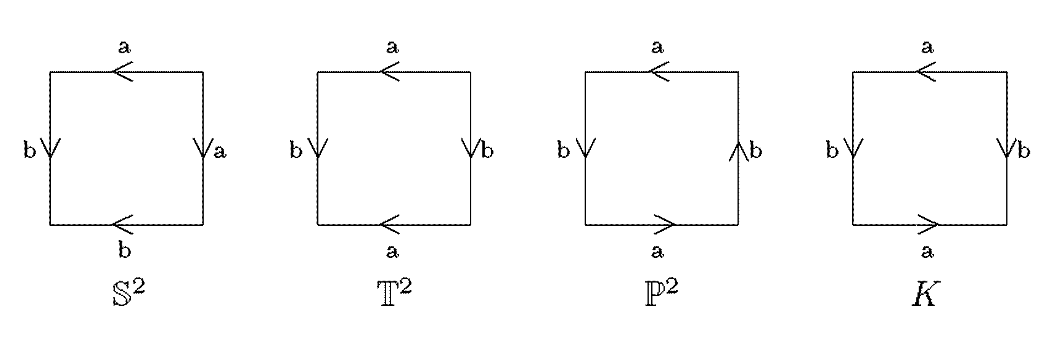
\includegraphics[width=0.9\textwidth]{img/realizacion-geom.png}
    \end{center}

    Si nos fijamos en la segunda realización geométrica, esta es claramente homeomorfa al cuadrado unidad $X=I \times I$ con la relación de equivalencia
    \[
        (x_1,y_1)\sim(x_2,y_2) \iff x_1-x_2\in\mathbb{Z}, y_1-y_2\in\mathbb{Z}
    \]
    que identifica los lados superior e inferior con la misma orientación y también derecho e izquierdo con la misma orientación. Este espacio cociente $\faktor{X}{\sim}$ es precisamente el que tratamos en un ejemplo de la Sección 1.2, donde se probó que era homeomorfo a $\mathbb{T}^2$.

    Queda como ejercicio probar que el resto de realizaciones geoométricas, es decir, cuadrados con una cierta relación de equivalencia, son homeomorfos a los espacios que se indica en la figura.
}

\propp{Compacidad y conexión de $|\partes|$}{
    Dada una representación poligonal $\partes$, su realización geométrica, $|\partes|$, es una superficie compacta. Además si solo tiene una palabra, entonces es conexa.
}{
    Vamos a ver que el espacio topológico cociente $\tilde{X}$ es:
    \begin{enumerate}
        \item Compacto
        \item Superficie ($T_2$, $2A\N$, localmente euclídeo)
    \end{enumerate}

    \underline{Compacto:} Sea $X$ el polígono en $\R^2$, sea $\sim$ la relación de equivalencia entre las aristas y sea $\tilde{X}$ el cociente. X es compacto y $p : X \to \tilde{X}=\faktor{X}{\sim}$ la proyección al cociente es continua. Por tanto, $\tilde{X}$ es compacto.

    \underline{$T_2$:} Puedo tomar discos en $\R^2$ infinitamente pequeños de forma que separen los puntos en $X$ y las imágenes por $p$ separan los puntos de $\tilde{X}$.

    \underline{$2A\N$:} La proyección es continua, y el polígono es $2A\N$, luego $\tilde{X}$ también lo es.

    \underline{Localmente euclídeo:} La idea es distinguir 3 casos: 

    Veamos que $\faktor{\partes}{R}$ es localmente euclídeo. Necesitamos que para cada punto, haya un entorno que sea homeomorfo a un abierto de $\R^2$. 
    Sea $x \in \faktor{\partes}{R}$ y consideramos 
    \[\pi^{-1}(x) = \begin{cases}
        p \in \text{int}(\partes) \\
        \{q_1, q_2\} \in \text{aristas} \\
        \{v_1, \dots, v_k\} \in \text{vértices}
    \end{cases}\]
    \begin{enumerate}
        \item $\pi^{-1}(x) = p \in \text{int}(P)$. Entonces, $\pi|_{\text{int}(\partes)} : \text{int}(\partes) \to \pi(\text{int}(\partes))$ es biyectiva y continua y su inversa también es continua. Por tanto, como $\text{int}(\partes)$ es abierto, se tiene que es localmente euclídeo en $\text{int}(\partes)$.
        \item Tomamos $D_i \subset \R^2$ disco centrado en $q_i$ con $\overline{D_1} \cap \overline{D_2} = \emptyset$. Además, tampoco cortan ningun vértice de $\partes$.
        Sea $U_i = D_i \cap \partes \equiv$ semidiscos. Sea $h : a \to a'$ el homeomorfismo que da la relación de equivalencia (con $a, a'$ las aristas), es decir, $h(x)=y, x \in a, y \in a' \iff xRy$. 
        
        Existen homeomorfismos $\alpha_i : \R^2 \to \R^2$ (de hecho aplicaciones afines) tales que: 
        \[\alpha_1(U_1) = \{z\in \mathbb{C} : |z| < r_1, \text{Im}(z) \ge 0\} = \{(x,y)\in\R^2 : \|(x,y)\| < r_1, y \ge 0\}\]
        \[\alpha_2(U_2) = \{z\in \mathbb{C} : |z| < r_2, \text{Im}(z) \le 0\}\]
        y también que $\alpha_2 \circ h = \alpha_1|_a$.
        
        Sea $r = \min\{r_1, r_2\}$ y llamo $V_1 = \alpha^{-1}(\{z : |z|<r, \text{Im}(z) \ge 0\})$ y $V_2 = \alpha^{-1}(\{z : |z|<r, \text{Im}(z) \le 0\})$. Lo que hemos llamado $A = V_1 \cup V_2$ abierto de $\partes$. $\alpha : V_1 \cup V_2 \to B(0,r)$ identificación (continua, cerrada, sobreyectiva) donde $\alpha(x) = \begin{cases}
            \alpha_1(x) & x \in V_1 \\
            \alpha_2(x) & x \in V_2
        \end{cases}$. Está bien definida y pasa al cociente porque $xRy, x\in a, y \in a' \implies y = h(x)$ y entonces $\alpha(y) = \alpha_2(y) = \alpha_2(h(x)) = \alpha_1(x) = \alpha(x)$. % Falta la demostración visual, con los segmentos y los discos que se transforman en un circulito en R^2
        \item Sea ahora $\pi^{-1}(x) = \{v_1, \dots, v_k\}, k \in \N$. Consideramos $D_i$ disco infinitamente pequeño tal que $\overline{D_i} \cap \overline{D_j} = \emptyset, i \neq j$ no contenga puntos de otras aristas, ni vértices. 
        Sea $U_i = D_i \cap \partes \equiv$ sector circular. Supongamos los sectores ordenados de forma que $b_i \sim a_{i+1}, i=1,\dots,k$.

        Objetivo: $V_1 \cup \dots \cup V_k \overset{\alpha}{\longrightarrow} B(0,r) \subset \R^2$. 
        %TODO: No se hacer el dibujo este de la proyección canónica, ayuda!!

        Sea homeomorfismo afín $\alpha_i : \R^2 \to \R^2$ que lleva $U_i$ en $\{z : |z| < r_i, \text{arg}(z) \in [\frac{2\pi(i-1)}{k}, \frac{2\pi i}{k}]\}$ para todo $i=1,\dots,k$ cumpliendo $\alpha_{i+1} \circ h_i = \alpha_i|_{b_i}$, donde $h_i : b_i \to a_{i+1}$.
        
        Finalmente queda construir $\alpha_k : \R^2 \to \R^2$ que lleve $U_k$ en $\{z : |z| < r_k, \text{arg}(z) \in [\frac{2\pi(k-1)}{k}, 2\pi]\}$ y que cumpla 
        \begin{equation}
            \label{5.3-casos} \begin{cases}
                \alpha_k \circ h_{k-1} = \alpha_{k-1}|_{b_{k-1}} \\
                \alpha_1 \circ h_k = \alpha_k|_{b_k \equiv a_1}
            \end{cases}
        \end{equation}, con $h_k : b_k \to a_1$.
        
        Para garantizar la existencia de $\alpha_k$, podemos construirla en dos pasos, una para llevar a su hueco y otra para garantizar \ref{5.3-casos}. 

        Sea $r \le \min{r_1, \dots, r_k}$ y $V_i = \alpha_i^{-1}(\{z : |z| < r, \text{arg}(z) \in [\frac{2\pi(i-1)}{k}, \frac{2\pi i}{k}]\})$. Definimos $\alpha : V_1 \cup \dots \cup V_k \to B(0,r)$ como $\alpha(x) = \alpha_i(x), x \in V_i$. $\alpha$ está bien definida pues si $xRy, x\in b_i, y \in a_{i+1} \implies \alpha(y) = \alpha_{i+1}(h_i(x)) = \alpha_i(x) = \alpha(x), i\ne k$. Y para $k$, $y = h_k(x) \in a_1 \to$ misma cuenta. Luego, $\alpha$ es identificación (continua, sobreyectiva, cerrada) y $\tilde{\alpha}$ es homeomorfismo.
    \end{enumerate}
}

\defn{Presentación de una superficie compacta}{
    Sea $\mathcal{S}$ una superficie compacta. Una presentación de $\mathcal{S}$ es una presentación poligonal $\partes$ tal que $|\partes|$ y $\mathcal{S}$ son homeomorfas.
}

\propp{Presentación de $\mathcal{S}_1\#\mathcal{S}_2$}{
    Sean $\mathcal{S}_1$ y $\mathcal{S}_2$ dos superficies compactas y conexas presentadas por $\langle A_1|W_1 \rangle$ y $\langle A_2|W_2 \rangle$, respectivamente. Entonces, $\langle A_1 \sqcup A_2|W_1W_2 \rangle$ es una presentación de $\mathcal{S}_1\#\mathcal{S}_2$.
}{
    Sea $\partes_1$ polígono asociado a $W_1$ y sean $p,q \in \text{int}(\partes_1)$ dos puntos distintos y $v$ vértice de $partes_1$. 

    $\mathcal{S}_1 = \langle A_1|W_1 \rangle = \langle A_1 \sqcup {a,b,c}|W_1cba = Q_1, abc \rangle$. Definimos $\pi' : \partes_1 \sqcup Q_1 \to \mathcal{S}_1$ y $\pi:\partes_1 \to \mathcal{S}_1$. Sea entonces $B_1 = \pi'(\text{int}(Q_1)) \subset \mathcal{S}_1$. Si probamos que $B_1$ es homeomorfo a un disco, entonces tendremos que $\mathcal{S}_1\#\mathcal{S}_2$ se puede ver como $\mathcal{S}_1 \setminus Q_1 \sqcup \faktor{\mathcal{S}_2}{R_\varphi}$.

    Para ver que $B_1$ es homeomorfo a un disco, hacemos un razonamiento similar al de la proposición anterior tomando como abierto uno de la forma "sector circular" con $p$ y $q$ dentro del sector y $v$ el vértice, y hacer el mismo razonamiento con un solo sector.

    Así, tendremos que $\langle A_1 \sqcup \{a,b,c\}|W_1cba, a^{-1}b^{-1}c^{-1} \rangle$ es una presentación de $\mathcal{S}_1\setminus \text{int}(Q_1)$, análogamente $\langle A_2 \sqcup \{a',b',c'\}|W_2c'b'a', (a')^{-1}(b')^{-1}(c')^{-1} \rangle$ es presentación de $\mathcal{S}_2\setminus \text{int}(Q_2)$.

    Para obtener $\mathcal{S}_1\#\mathcal{S}_2$ identificamos $\varphi : \partial Q_1 \to \partial Q_2$, con $\varphi(a) = a', \varphi(b) = b', \varphi(c) = c'$ y obtenemos $\mathcal{S}_1\#\mathcal{S}_2 = \langle A_1 \sqcup A_2 \sqcup \{a,b,c\}|W_1cbaa^{-1}b^{-1}c^{-1}W_2\rangle = \langle A_1 \sqcup A_2|W_1W_2\rangle$.
}

\clearpage

\section{Transformaciones elementales}

\defn{Transformaciones elementales sobre presentaciones poligonales}{
    Dada una presentación poligonal, llamaremos transformaciones elementales a las siguientes operaciones:
    \begin{itemize}
        \item \textbf{Renombrado:} Sustituir todas las apariciones de una letra $a$ por otra letra $b$ que no estuviera en la presentación.
        \item \textbf{Subdivisión:} Cambiar todas las apariciones de una letra $a$ por $ab$, y todas las apariciones de $a^{-1}$ por $b^{-1}a^{-1}$, donde $b$ es una letra nueva que no estaba en la presentación.
        \item \textbf{Consolidado: } Dadas dos letras $a$ y $b$ que siempre aparezcan juntas de la forma $ab$ o $b^{-1}a^{-1}$, sustituimos todas las apariciones de $ab$ por $c$, y todas las apariciones de $b^{-1}a^{-1}$ por $c^{-1}$, donde $c$ es una letra nueva que no estaba en la presentación.
        \item \textbf{Reflejo: } Cambiar una palabra de la forma $a_1a_2\dots a_k$ por $a_k^{-1}a_{k-1}^{-1}\dots a_1^{-1}$, donde $a_i$ son letras de la presentación.
        \item \textbf{Rotación: } Cambiar una palabra de la forma $a_1a_2\dots a_k$ por $a_2a_3\dots a_k a_1$, donde $a_i$ son letras de la presentación.
        \item \textbf{Corte:} Dada una palabra $W_1W_2$, con $W_1$ y $W_2$ no vacías, quitamos $W_1W_2$ de la presentación y añadimos $W_1a, a^{-1}W_2$ como palabras nuevas, donde $a$ es una letra nueva que no estaba en la presentación.
        \item \textbf{Pegado} Sustituimos dos palabras de la forma $W_1a, a^{-1}W_2$, con $W_1$ y $W_2$ arbitrarias y no vacías, por $W_1W_2$.
        \item \textbf{Plegado} Una palabra de la forma $W_1aa^{-1}$ se sustituye por $W_1$, donde $W_1$ tiene al menos longitud 3, salvo que haya una sola palabra, en cuyo caso podría ser de dos letras.
        \item \textbf{Desplegado} Una palabra de la forma $W_1$ se sustituye por $W_1aa^{-1}$, donde $W_1$ tiene al menos longitud 3, salvo que haya una sola palabra, en cuyo caso podría ser de dos letras.
    \end{itemize}
}

\defn{Presentaciones equivalentes}{
    Dos transformaciones poligonales se dice que son topológicamente equivalentes si sus realizaciones geométricas son homeomorfas.
}

\propp{Equivalencia por transformaciones elementales}{
    Cada una de las transformaciones elementales sobre una presentación poligonal produce otra presentación topológicamente equivalente. 
}{Pendiente.}

\clearpage

\section{Teorema de Clasificación}

En esta sección se presenta y demuestra el teorema de clasificación de superficies compactas de $\R ^n$. Ya hemos visto que las transformaciones elementales sobre presentaciones poligonales producen presentaciones equivalentes, nuestro objetivo ahora es demostrar que cualquier presentación poligonal de una superficie compacta y conexa puede ser transformada en una de las formas canónicas dadas por el teorema de clasificación.

El siguiente lema simplifica la demostración del teorema de clasificación, mostrando la equivalencia entre ciertos tipos de superficies.

\lemp{Equivalencia entre algunos tipos de superficies}{
    \label{lem:toro-proyectivo}
    \begin{enumerate}
        \item La botella de Klein y $\mathbb{RP}^2\#\mathbb{RP}^2$ son homeomorfas.
        \item $\mathbb{T}^2\#\mathbb{RP}^2$ y $\mathbb{RP}^2\#\mathbb{RP}^2\#\mathbb{RP}^2$ son homeomorfas.
    \end{enumerate}
}{
    Para la primera parte nos fijamos en el siguiente dibujo:
    \begin{center}
        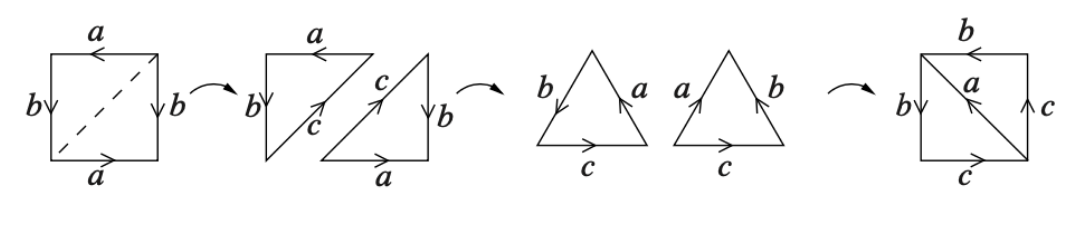
\includegraphics[width=0.8\textwidth]{img/botella-klein-transformacion.png}
    \end{center}
    Por tanto a la presentación de la botella de Klein dada por $\langle a,b\mid abab^{-1} \rangle$ le aplicamos un corte, una reflexión, dos rotaciones, un pegado y una última rotación:
    \begin{align*}
        \langle a,b\mid abab^{-1} \rangle &\cong \langle a,b,c\mid abc, c^{-1}ab^{-1} \rangle \cong \langle a,b,c\mid abc,ba^{-1}c \rangle \\
        &\cong \langle a,b,c\mid bca,a^{-1}cb \rangle \cong \langle b,c\mid bccb \rangle \cong \langle b,c\mid bbcc \rangle
    \end{align*}
    y llegamos a una presentación de la suma conexa de dos proyectivos.

    Para la segunda parte nos fijamos en este otro dibujo:
    \begin{center}
        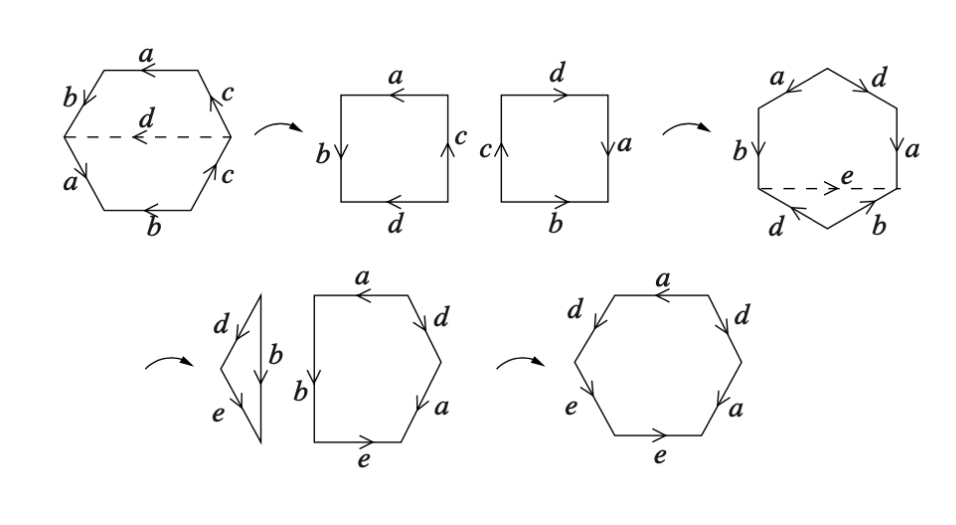
\includegraphics[width=0.6\textwidth]{img/toro-proyectivo-transformacion.png}
    \end{center}
    Partimos de una presentación de $K\#\mathbb{RP}^2$, que por la parte 1 sabemos que es homeomorfo a $\mathbb{RP}^2\#\mathbb{RP}^2\#\mathbb{RP}^2$. La presentación está dada por $\langle a,b\mid abab^{-1}cc \rangle$, y le aplicamos las transformaciones de la figura (ejercicio para el lector: indicar qué transformaciones elementales se usan en cada paso)
    \begin{align*}
        \langle a,b,c\mid abab^{-1}cc \rangle &\cong \langle a,b,c,d\mid abd^{-1}c, c^{-1}ba^{-1}d^{-1} \rangle \cong \langle a,b,d\mid abd^{-1}ba^{-1}d^{-1} \rangle \\
        &\cong \langle a,b,d,e\mid deb^{-1},bea^{-1}d^{-1}a \rangle \cong \langle a,d,e \mid deea^{-1}d^{-1}a \rangle\\
        &\cong \langle a,d,e \mid a^{-1}d^{-1}adee \rangle
    \end{align*}
    y llegamos a una presentación de la suma conexa de un toro y un proyectivo.
}

\thm{Clasificación de superficies compactas}{
    Sea $S$ una superficie compacta y conexa, entonces $S$ es homeomorfa a una de las siguientes superficies:
    \begin{itemize}
        \item la esfera $\mathbb{S}^2$.
        \item una suma conexa de toros $\mathbb{T}^2\#\dots\#\mathbb{T}^2$.
        \item una suma conexa de planos proyectivos $\mathbb{RP}^2\#\dots\#\mathbb{RP}^2$.
    \end{itemize}
}
\pf{
    \noindent
    Sea $M$ una superficie compacta y conexa y sea $\partes$ su presentación poligonal, la cual sabemos que existe por el Teorema de Radó (\ref{thm:rado}).

    \vspace{1em}
    \noindent
    \underline{Objetivo:} aplicar transformaciones elementales a $\partes$ hasta llegar a uno de los siguientes casos:
    \[
        \partes \cong 
        \begin{cases}
            \langle a \vert a a^{-1} \rangle, & \text{presentación de } \mathbb{S}^2, \\[6pt]
            \langle a_1, b_1, \dots, a_n, b_n \vert a_1b_1a_1^{-1}b_1^{-1}\dots a_n b_n a_n^{-1}b_n^{-1} \rangle, 
            & \text{presentación de } \mathbb{T}^2\#\dots\#\mathbb{T}^2, \\[6pt]
            \langle a_1, \dots, a_n \vert a_1a_1\dots a_n a_n \rangle, 
            & \text{presentación de } \mathbb{RP}^2\#\dots\#\mathbb{RP}^2.
        \end{cases}
    \]

    \vspace{1em}
    \noindent
    Para ello, separamos la demostración en 7 pasos, en cada uno de los cuales manipulamos $\partes$ para que cumpla una determinada condición 
    (nótese el abuso de notación al llamar $\partes$ tanto a la presentación original como a la presentación $\partes '$ obtenida tras aplicar una transformación elemental). 
    Al término del último paso, llegaremos a que $\partes$ adopta una de las formas canónicas anteriores.

    \vspace{1em}
    \noindent
    Durante la demostración, llamaremos \emph{aristas complementarias} a aquellas que aparecen en $\partes$ como $a$ y $a^{-1}$, y 
    \emph{aristas retorcidas} a las que aparecen como $a$ y $a$, o $a^{-1}$ y $a^{-1}$.

    \vspace{1.3em}
    \noindent
    \underline{PASO 1:}
    \begin{quote}
        Podemos suponer que $\partes$ tiene solo una palabra (o que el polígono tiene 1 sola cara).
    \end{quote}

    \noindent
    Una consecuencia de que la superficie sea conexa es la siguiente: si $\partes$ tiene varias palabras, para cada palabra debe existir una arista que se identifique con una arista de otra palabra. 
    Es decir, siempre que $\partes$ tenga varias palabras, para cada palabra $W_1$ de $\partes$ debe existir una arista $a \in W_1$ y una palabra $W_2$ tal que 
    o bien $a\in W_2$ o $a^{-1}\in W_2$. En caso de que esto no ocurra, en la realización geométrica $W_1$ y las demás palabras serían disjuntas, formando así una separación que
    contradice la conexión de $M$.

    \vspace{0.5em}
    \noindent
    Ahora, si $W_1$ es una palabra y $\partes$ tiene más de una palabra, por lo anterior existe una arista $a$ que conecta con otra palabra $W_2$ 
    (ya sea mediante $a$ o $a^{-1}$). Pegando $W_1$ y $W_2$ (aplicando rotaciones y reflejos si fuera necesario), 
    obtenemos una presentación donde $W_1$ y $W_2$ se han sustituido por una única nueva palabra $W_1'W_2'$. 

    \vspace{0.5em}
    \noindent
    Como el número de palabras de la presentación original es finito, mediante este proceso se obtiene una presentación equivalente compuesta por una sola palabra.

    \vspace{1.3em}
    \noindent
    \underline{PASO 2:}
    \begin{quote}
        Podemos suponer que no hay pares de aristas complementarias adyacentes ($W_1aa^{-1}W_2$).
    \end{quote}

    \noindent
    Si las hubiera, plegando por ellas desaparecen. Excepto el caso en que solo tengamos ese par ($W_1, W_2 = \emptyset$). 
    Pero entonces la superficie es una esfera, que es una de las formas canónicas que pretendíamos obtener.

    \vspace{1.3em}
    \noindent
    \underline{PASO 3:}
    \begin{quote}
        Podemos suponer que todos los pares de aristas retorcidas son adyacentes.
    \end{quote}

    \noindent
    Supongamos que tenemos $VaWa$, con $V,W \ne \emptyset$. Cortamos por el medio ($Vab$ y $b^{-1}Wa$). 
    Rotamos y reflejamos la segunda palabra ($bVa$ y $a^{-1}W^{-1}b$), y pegamos por $a$ llegando a $bbVW^{-1}$, donde las aristas retorcidas ya son adyacentes. 
    La repetición de este proceso una cantidad finita de veces demuestra el paso 3.

    \vspace{0.5em}
    \noindent
    \textit{Nota:} En cada iteración, es posible que tengamos que volver a aplicar el paso 2 ya que al pegar $V$ y $W^{-1}$ en $VW^{-1}$ podrían aparecer nuevas aristas complementarias adyacentes.

    \vspace{1.3em}
    \noindent
    \underline{PASO 4:}
    \begin{quote}
        Podemos suponer que el polígono tiene todos sus vértices identificados.
    \end{quote}

    \noindent
    Sea $p:\partes \to M$ la proyección al cociente. Sea $p(v)=[v]$. 
    Si no todos los vértices están identificados, existen vértices $v_1, w$ en $\partes$ 
    y una arista $ a : v_1 \to w$ con $p(v_1)\ne p(w)$. 
    Ahora, la arista que termina en $v_1$ no puede ser ni $a$ (porque entonces $p(v_1) = p(w)$) 
    ni $a^{-1}$ (pues tendríamos la secuencia $a^{-1} a$ y al aplicar de nuevo el paso 2 llegaríamos también a que $p(v_1) = p(w)$). 
    Por tanto, concluimos que la arista es distinta, llamémosla $b$, y al vértice del que parte $x$. 
    Es decir, tenemos $b : x \to v_1$.

    \vspace{0.5em}
    \noindent
    Por la definición de presentación poligonal, la letra $b$ debe aparecer (bien como $b$ o como $b^{-1}$) en otro sitio de la presentación. 
    Suponemos que aparece $b^{-1}$ (si fuese $b$ sería análogo salvo una reflexión que ahora mencionaremos). 
    Tenemos entonces por construcción la secuencia $baXb^{-1}Y$, con $X$ e $Y$ cadenas arbitrarias de la presentación. Podemos suponer $X,Y \ne \emptyset$. Veámos por qué:
    \begin{itemize}
        \item Si $X$ fuese vacío, por la definición de $b$, el vértice al que llega $b^{-1}$ en nuestra cadena no sería otro que $w$ (recordemos $a:v_1\to w$). 
              Pero entonces $p(v_1) = p(w)$, lo que contradice la hipótesis.
        \item Si $Y$ fuese vacío, rotando obtendríamos dos aristas adyacentes $b$ y $b^{-1}$ y estaríamos en el paso 2.
    \end{itemize}

    \vspace{0.5em}
    \noindent
    Ahora, cortando por una nueva arista $c : w \to x$, rotando para pegar por $b$ 
    (y reflejando si en vez de tener $b^{-1}$ tuviéramos $b$) obtenemos:
    \[
        baXb^{-1}Y \;\cong\; bac \text{, } c^{-1}Xb^{-1}Y \;\cong\; acb \text{, } b^{-1}Yc^{-1}X \;\cong\; acYc^{-1}X
    \]

    \noindent
    Incluyendo los vértices en la presentación a la que hemos llegado, 
    \[
        v_1 \overset{a}{\to} w \overset{c}{\to} x \overset{Y}{\to} x \overset{c^{-1}}{\to} w \overset{X}{\to} v_1
    \]
    que es una presentación equivalente donde hemos reducido la cantidad de vértices que se identifican con $v_1$ en una unidad.

    \vspace{0.5em}
    \noindent
    \textit{Nota:} De nuevo, podría ser que al pegar $X a$ aparecieran nuevas aristas complementarias adyacentes. 
    En ese caso, se aplicaría el paso 2, donde en ningún caso se pueden aumentar los vértices identificados con $v_1$, solo disminuirlos.

    \vspace{0.5em}
    \noindent
    Una cantidad finita de iteraciones de este proceso elimina la clase de equivalencia de vértices $v_1$, 
    pues en cada paso se elimina un elemento de este conjunto finito. 
    Repitiendo para cada clase de equivalencia de vértices, llegamos a que solo puede quedar una, 
    demostrando así el paso 4.

    \vspace{1.3em}
    \noindent
    \underline{PASO 5:}
    \begin{quote}
        Se cumple que si aparece un par $a, a^{-1}$, entonces hay otro par $b, b^{-1}$ intercalado, 
        es decir, de la forma $a\dots b\dots a^{-1} \dots b^{-1}$.
    \end{quote}

    \noindent
    Si no fuese así, tendríamos una presentación de la forma $aXa^{-1}Y$, donde además $X$ e $Y$ no comparten aristas 
    (si compartiesen alguna letra $b$, por hipótesis ésta debería aparecer como $b$, y no como $b^{-1}$, tanto en $X$ como en $Y$, 
    lo cual no es posible por el paso 3). 
    Esto significa también que $X$ e $Y$ no comparten vértices, ya que si $x$ fuese un vértice de $X$ y $y$ un vértice de $Y$ tales que acaban identificados en la proyección,
    por cómo se define la relación de equivalencia tendría que haber una arista a la vez en $X$ y en $Y$, contradiciendo así que $X$ e $Y$ no comparten aristas.

    \vspace{0.5em}
    \noindent
    En particular, los vértices finales de $a$ y $a^{-1}$, que están ambos en $X$, 
    solo pueden identificarse con vértices de $X$. 
    Por otro lado, los vértices iniciales de $a$ y $a^{-1}$, que están ambos en $Y$, 
    solo pueden identificarse con vértices de $Y$. 
    Entonces, existen dos clases de equivalencia de vértices distintas, 
    lo que contradice el paso 4.

    \vspace{0.5em}
    \noindent
    \textit{Nota:} se invita al lector a hacer el dibujo y verlo por sí mismo, en este caso no es difícil. No se puede confirmar ni desmentir que la invitación al lector sea por la pereza de los autores de añadir dibujos. 

    \vspace{1.3em}
    \noindent
    \underline{PASO 6:}
    \begin{quote}
        Podemos suponer que los pares de aristas del paso 5 aparecen consecutivos.
    \end{quote}

    \noindent
    Tenemos ahora una cadena $aXbYa^{-1}Zb^{-1}W$, 
    y buscamos hacer transformaciones para que las aristas aparezcan consecutivas. 
    Empezamos con nuestra presentación original, la cual rotamos para cortar desde el final de $X$ al final de $W$, llamando a la arista del corte $c$. 
    \[
        aXbYa^{-1}Zb^{-1}W \cong WaXbYa^{-1}Zb^{-1} \;\;\cong\;\; WaXc \text{, } c^{-1}bYa^{-1}Zb^{-1}
    \]
    \noindent 
    Vamos a pegar por $a$, para lo cual tenemos primero que rotar.
    \[
        WaXc \text{, } c^{-1}bYa^{-1}Zb^{-1} \cong XcWa \text{, } a^{-1}Zb^{-1}c^{-1}bY \;\;\cong\;\; XcWZb^{-1}c^{-1}bY
    \] 
    \noindent
    Ahora cortamos desde el final de $b^{-1}$ al final de $c$, llamando $d$ a esa arista. 
    \[
        XcWZb^{-1}c^{-1}bY \;\;\cong\;\; c^{-1}bYXcWZb^{-1} \;\;\cong\;\; c^{-1}bYXcd \text{, } d^{-1}WZb^{-1}
    \]

    \noindent
    Por último, rotando y pegando por $b$ conseguimos que las cuatro aristas queden consecutivas.
    \[
        c^{-1}bYXcd \text{, } d^{-1}WZb^{-1} \cong YXcdc^{-1}b \text{, } b^{-1}d^{-1}WZ \;\;\cong\;\; YXcdc^{-1}d^{-1}WZ
    \]

    \vspace{0.5em}
    \noindent
    Haciendo esto para todos los pares de aristas intercalados que no sean consecutivos se demuestra el paso 6.

    \vspace{1.3em}
    \noindent
    \underline{PASO 7:}
    \begin{quote}
        La superficie $M$ es homeomorfa a $\mathbb{T}^2\#\dots\#\mathbb{T}^2$, o bien a $\mathbb{RP}^2\#\dots\#\mathbb{RP}^2$.
    \end{quote}

    \noindent
    Con todo lo que hemos hecho hasta ahora, nuestra presentación solo puede contener los siguientes tipos de elementos:

    \begin{enumerate}
        \item Parejas de aristas complementarias consecutivas, de la forma $aba^{-1}b^{-1}$.
        \item Aristas retorcidas de la forma $aa$.
    \end{enumerate}

    \noindent
    Recordemos que la presentación poligonal de un toro viene dada precisamente por la forma $a b a^{-1} b^{-1}$, 
    y la presentación de un plano proyectivo por $aa$. 
    Por tanto, si solo hubiese aristas de una de estas dos formas, 
    la superficie sería homeomorfa a una suma conexa de toros o de planos proyectivos, respectivamente.

    \vspace{0.5em}
    \noindent
    Nos queda ver qué ocurre en el caso de que $\partes$ contenga ambos grupos de aristas. 
    Supongamos que existen un grupo de aristas complementarias $aba^{-1}b^{-1}$ y otro de aristas retorcidas $cc$. 
    Por el lema \hyperref[lem:toro-proyectivo]{2.6.1}, la suma conexa de un toro y un plano proyectivo es homeomorfa a la suma conexa de tres planos proyectivos. 
    Es decir, $aba^{-1}b^{-1}cc \cong a'a'b'b'c'c'$. 
    Transformando cada par (toro, proyectivo) en tres proyectivos podemos eliminar los toros y quedarnos con un número finito de planos proyectivos.

    \vspace{0.5em}
    \noindent
    Concluyendo, si $\partes$ tiene solo aristas complementarias alternadas, es homeomorfa a una suma conexa de toros. 
    Si tiene solo aristas retorcidas, es homeomorfa a una suma conexa de planos proyectivos. 
    Y si tiene ambos tipos de aristas, es homeomorfa a una suma de planos proyectivos.
}

\propp{Característica de Euler invariante por transformaciones elementales}{
    La característica de Euler de una presentación poligonal es invariante por transformaciones elementales
}{
    \noindent Renombrar, reflejar y rotar CHECK

    \noindent Consolidar y dividir:

    \[ \text{3 vertices, 2 aristas $\longleftrightarrow$ 2 vértices, 1 arista, $\chi$ se mantiene.} \]

    \noindent Cortar y pegar:

    \[\text{1 cara, 2 aristas $\longleftrightarrow$ 2 caras, 3 aristas, $\chi$ se mantiene.}\]

    \noindent Plegar y desplegar:

    \[\text{1 vértice $\longleftrightarrow$ 2 vértices, 1 arista, $\chi$ se mantiene.}\]
}

\defn{Característica de Euler de una superficie compacta}{
    Dada una superficie compacta $M$, se define su característica de Euler $\chi(M)$ como la característica de cualquier presentación poligonal de ella (ya que es invariante por transformaciones elementales).
}

\ex{
    Característica de Euler en las superficies modelo:
    \begin{enumerate}
        \item $\chi(\mathbb{S}^2) = 1-1+2 = 2$.
        \item $\chi(n\mathbb{T}^2) = 1-2n+1 = 2-2n$.
        \item $\chi(n\mathbb{RP}^2) = 1-n+1 = 2-n$.
    \end{enumerate}
}

\rmkb{
    Para todo poliedro de $\R^3$, esto es, un sólido bordeado por un conjunto finito de polígonos convexos unidos por los lados, que sea homeomorfo a la esfera $\mathbb{S}^2$ se tiene que
    \[ \chi = V - E + F = 2 \]
}

\defn{Superficie orientable}{
    Una superficie compacta se dice orientable si admite una presentación poligonal en la que no existe ningún par de aristas que se identifiquen recorriéndose en el mismo sentido, es decir, si para cada arista $a$ de la presentación, aparece tanto $a$ como $a^{-1}$.
}

\propp{}{
    Una superficie compacta no orientable contiene un subespacio homeomorfo a la cinta de Möbius (de hecho es un si y solo si).
}{
    \noindent ($\implies$) Siempre tenemos aristas identificadas $aa$.
    Demostración con dibujitos, no puedo hacerlo :(
    
    \noindent ($\impliedby$) Sea una presentación:
    
    \noindent\underline{Afirmación 1:} El subespacio homeomorfo a la cinta de Möbius toca al borde. No entra en detalle, si alguien quiere hacerlo que se las apañe jeje.
}

\ex{
    \noindent Superficies no orientables: $\mathbb{RP}^2$, $K$ (la botella).
    
    \noindent Superficies orientables: $\mathbb{S}^2$, $\mathbb{T}^2$.
}

\propp{Orientabilidad de la suma conexa}{
    Dadas dos superficies compactas $S_1$ y $S_2$, la suma conexa $S_1\# S_2$ es orientable si, y solo si, ambas superficies son orientables.
}{
    Pendiente...
}

\ex{
    $\mathbb{T}^2 \# \dots \# \mathbb{T}^2$ es orientable.
    $\mathbb{RP}^2 \# \dots \# \mathbb{RP}^2$ es no orientable.
}

\corp{
    Dos superficies compactas y conexas son homeomorfas si, y solo si, tienen la misma característica de Euler y la misma orientabilidad.
}{
    Pendiente...
}

\defn{Género de una superficie}{
    Sea $S$ una superficie compacta y conexa. Se define el género de $S$ como $g(S) = 1-\frac{1}{2}\chi(S)$ si $S$ es orientable, y $g(S) = 2 - \chi(S)$ si no lo es. El género también se conoce como el número de agujeros.
}

\ex{
    \begin{itemize}
        \item $g(\mathbb{S}^2) = 0 = g(0\mathbb{T})$.
        \item $g(\mathbb{T}^2 \# \dots \# \mathbb{T}^2) = n$.
        \item $g(\mathbb{RP}^2 \# \dots \# \mathbb{RP}^2) = n$.
    \end{itemize}
}

\corp{
    Si $S$ es una superficie compacta, conexa y orientable, entonces $S$ es homeomorfa a:
    \[\begin{cases}
        \text{una esfera, cuando $g(S) = 0$} \\
        \text{una suma conexa de $n$ toros, cuando $g(S) = n, n \ge 1$}
    \end{cases}\]
}{
    Pendiente...
}

\chapter{Homotopía. El grupo fundamental}

\section{Equivalencia homotópica}

\defn{Camino o arco}{
    Sea ($X,\tau$) un espacio topológico e $I = [0,1] \subset \R$. Se llama \textbf{camino o arco} en $X$ a una aplicación continua $\alpha: I \to X$. Se llama $\alpha(0)$ origen y $\alpha(1)$ final. Diremos que $\alpha$ es un arco uniendo $\alpha(0)$ con $\alpha(1)$. Cuando $\alpha(0) = \alpha(1)$ diremos que $\alpha$ es un lazo.
}

\defn{Aplicaciones homotópicas}{
    Dos aplicaciones continuas $f ,g : X \to Y$ entre dos espacios topológicos son homotópicas si existe una aplicación continua $F : X \times [0,1] \to Y$ tal que $F(x,0) = f(x)$ y $F(x,1) = g(x)$, para todo $x \in X$. Se dice que $F$ es una homotopía entre $f$ y $g$, y se representa por $f \simeq g$.
}

\rmkb{
    Si $F$ es una homotopía, para cada $t \in [0,1]$, definimos $F_t : X \to Y$ por $F_t(x) = F(x,t)$. Las aplicaciones $F_t$ son continuas, $F_0 = f$ y $F_1 = g$. Si fijamos $x$, entonces
    \[
    F_x(t) = F(x,t) : I \to Y
    \]
    es un arco en $Y$ uniendo $f(x)$ con $g(x)$.
}

\clearpage

\ex{
    Si $Y\subset \R^n$ es convexo, cualquier par de aplicaciones $f,g$ continuas son homotópicas.
}

\pf{
    Consideremos la siguiente homotopía:
    \[
    F:X\times I \to Y,\quad F(x,t)=tg(x)+(1-t)f(x)
    \]
    como para cada $x\in X$ se tiene $f(x),g(x)\in Y$ y el conjunto $Y$ es convexo, entonces el segmento contenido entre $f(x),g(x)$ está contenido en $Y$, luego $F$ está bien definida. Además es continua por ser composición de aplicaciones continuas. Finalmente notemos que $F(x,0)=f(x),F(x,1)=g(x)$.
}

\ex{
    Sean $X, Y$ espacios topológicos e $y_1, y_2 \in Y$. Entonces las aplicaciones constantes
    \[
    C_{y_i} : X \to Y,\quad C_{y_i}(x) = y_i,\quad i=1,2
    \]
    son homotópicas si y solo si existe un arco en $Y$ uniendo $y_1, y_2$.
}

\pf{
    Si ambas aplicaciones son homotópicas sea $F(x,t)$ la homotopía entre ellas, entonces dado $x_0\in X$ arbitrario la aplicación $F_{x_0}(t)=F(x_0,t)$ es un camino que une $y_1,y_2$ puesto que es continua y
    \[
    F_{x_0}(0)=F(x_0,0)=C_{y_1}(x_0)=y_1,\quad F_{x_0}(1)=F(x_0,1)=C_{y_2}(x_0)=y_2.
    \]

    Si por el contrario existe $\alpha:I\to Y$ un camino uniendo $y_1=\alpha(0),y_2=\alpha(1)$ entonces consideremos la aplicación dada por
    \[
    F(x,t)=\alpha(t)
    \]
    que es claramente continua y además verifica $F(x,0)=y_1=C_{y_1}(x), F(x,1)=y_2=C_{y_2}(x)$, luego es una homotopía.
}

\propp{Relación $\simeq$ entre aplicaciones continuas}{
    La propiedad de ser homotópicas $\simeq$ es una relación de equivalencia en el conjunto $\mathcal{C}(X,Y)$ formado por todas las aplicaciones continuas de $X$ en $Y$. 
}{
    \textbf{1. Reflexiva:} $f \simeq f$

    Definamos la aplicación $F:X\times I\to Y$ por $F(x,t) = f(x)$. $F$ es continua por ser $f$ continua, además se tiene
    $\begin{cases}
        F(x,0) = f(x) \\
        F(x,1) = f(x)
    \end{cases}$
    por lo que es una homotopía, luego $f\simeq f$.

    \clearpage

    \noindent\textbf{2. Simétrica:} $f \simeq g \implies g \simeq f$
    
    Sea $F$ la homotopía entre $f,g$ entonces la aplicación
    \[
        \overline{F}:X\times I \to Y,\quad 
        \overline{F}(x,t) = F(x,1-t)
    \]
    es una homotopía entre $g,f$ puesto que es continua al serlo $F$ y cumple $\overline{F}(x,0)=F(x,1)=g(x), \overline{F}(x,1)=F(x,0)=f(x)$. 
    
    \textit{Nota:} La aplicación $\overline{F}$ se puede construir con cualquier homeomorfismo $\alpha : I \to I$ con $\alpha(0) = 1$ y $\alpha(1) = 0$ en vez de $1-t$.

    \noindent\textbf{3. Transitiva:} $f \simeq g,g \simeq h \implies f \simeq h$
    
    Sea $F_1$ la homotopía entre $f,g$ y $F_2$ la homotopía entre $g,h$, entonces la aplicación
    \[
    \overline{F}:X\times I \to Y,\quad
    \overline{F}(x,t) =\begin{cases}
        F_1(x,2t) & t \in [0, \frac{1}{2}] \\
        F_2(x,2t-1) & t \in [\frac{1}{2}, 1]
    \end{cases}
    \]
    es continua y verifica $\overline{F}(x,0)=F_1(x,0)=f(x), \overline{F}(x,1)=F_2(x,1)=h(x)$, por lo que es una homotopía entre $f$ y $h$.
    
    \textit{Nota:} Al igual que antes, se podría hacer con cualquier homeomorfismo que cumpla con lo que necesitamos.
}

\defn{Espacios homotópicamente equivalentes}{
    Decimos que dos espacios topológicos $X$ e $Y$ son homotópicamente equivalentes o tienen el mismo tipo de homotopía (denotado $X \simeq Y$) si existen aplicaciones continuas $f : X \to Y$ y $g :Y \to X$ tales que $g \circ f \simeq Id_X$ y $f \circ g \simeq Id_Y$. A la aplicación $f$ (también a $g$) se le llama, equivalencia de homotopía.
}

\ex{
    Si $Y \subset \R^n$ es convexo, entonces $Y \simeq \{x\}$.
}

\pf{
    Sea $X=\{x\}$, fijemos un $y_0\in Y$ y definamos las aplicaciones $f : X \to Y,\quad f(x)=y_0$ y $g : Y \to X,\quad g(y)=x$. Es inmediato notar que $g\circ f=Id_X$ puesto que para el único punto de $X$ se cumple
    \[
    g(f(x))=g(y_0)=x.
    \]
    Por tanto $g\circ f=Id_X\simeq Id_X$ por la reflexividad de $\simeq$.
    
    Por otro lado sea $h=f\circ g:Y\to Y$ y definamos la siguiente homotopía:
    \[
    H(y,t)= (y,t) = ty + (1-t)y_0 \implies
    \begin{cases}
        H(y,0) = y_0 = f(x) = f(g(y)) = h(y) \\
        H(y,1) = y = Id_Y(y)
    \end{cases}
    \]
    que es claramente continua y está bien definida porque $Y$ es convexo. 
}

\ex{
    $\R^2\setminus\{0\} \simeq \mathbb{S}^1$.
}

\pf{
    Buscamos $f : \R^2\setminus\{0\} \to \mathbb{S}^1$ y $g : \mathbb{S}^1 \to \R^2\setminus\{0\}$ continuas tales que
    \[
    \begin{cases}
        f \circ g \simeq Id_{\mathbb{S}^1} \\
        g \circ f \simeq Id_{\R^2\setminus\{0\}}.
    \end{cases}
    \]
    
    Sean $f(y) = \frac{y}{|y|}$ y $g(x) = x$. Es inmediato notar que $f\circ g= Id_{\mathbb{S}^1} \simeq Id_{\mathbb{S}^1}$ ya que \[
    f(g(x))=f(x)=\frac{x}{|x|}=x
    \]
    al ser $g(x)=x$ de norma 1.
    
    Por otro lado definamos la homotopía $F$ siguiente
    \[
        F(y,t)=ty + (1-t)\frac{y}{|y|},\quad
        \begin{cases}
            F(y,0) = \frac{y}{|y|}=g(f(y)) \\
            F(y,1) = y = Id_{\R^2\setminus\{0\}}(y)
        \end{cases}
    \]
    luego $g\circ f\simeq Id_{\R^2\setminus\{0\}}$.
}

\ex{
    La corona circular $C = \{(x,y) \in \R^2 : 1 \le x^2 +y^2 \le 2\} \simeq \mathbb{S}^1$
}
\pf{
    Procedemos de forma idéntica al ejemplo anterior. De hecho, se recomienda al lector intentar hacerlo como ejercicio antes de ver la solución.
    
    Definimos $f:C \to \mathbb{S}^1$, $g:\mathbb{S}^1 \to C$ como sigue:
    \begin{center}
        $f(y) = \frac{y}{|y|}$ \quad,\quad  $g(x) = x$
    \end{center}
    Para cualquier $x \in \mathbb{S}^1 $ se tiene que 
    \[
        f \circ g (x) = f(x) = x
    \] 
    Concluimos que  $f \circ g \simeq Id_{\mathbb{S}^1}$. Por otro lado, si $y \in C$, 
    \[
    g\circ f (y) = g(\frac{y}{|y|}) = \frac{y}{|y|}
    \]
    Consideramos la homotopía $F : C \times I \to C$ siguiente, 
    \[
        F(y, t) = ty + (1 - t) \frac{y}{|y|}, \quad
        \begin{cases}
            F(y,0) = \frac{y}{|y|}=g(f(y)) \\
            F(y,1) = y = Id_{\mathbb{S}^1 
            }(y)
        \end{cases}
    \]
    Se puede comprobar fácilmente que para cualquier $y\in C$ la aplicación $F_y$ definida como $F_y(t) = F(y, t)$ verifica $F_y(t) \in C \quad \forall t \in I $. Así, $F$ está bien definida y por tanto $g\circ f \simeq Id_C$.
}


\propp{Espacios homeomorfos y homotopía}{
    Si $X$ e $Y$ son homeomorfos, entonces $X \simeq Y$. El recíproco no es cierto.
}{
    Supongamos que $X$ e $Y$ son homeomorfos. En tal caso existe $f:X \to Y$ homeomorfismo, que será una aplicación continua y con inversa $g=f^{-1}$ también continua. Entonces
    \[
    g\circ f=Id_{X}\simeq Id_X,\quad f\circ g=Id_{Y}\simeq Id_{Y}
    \]
    por lo que $X\simeq Y$.

    Como contraejemplo para el recíproco consideremos el conjunto $\R^n$ que es convexo, por tanto $\R^n\simeq \{x\}$ para cualquier $x\in\R^n$, sin embargo no son espacios homeomorfos puesto que $\R^n$ no es compacto y $\{x\}$ sí.
}

\propp{Relación $\simeq$ entre espacios}{
    La propiedad $\simeq$ define una relación de equivalencia entre los espacios topológicos.
}{
    \textbf{1. Reflexiva:} $X \simeq X$
    
    Basta tomar $f = g = Id_X \implies f \circ g = g \circ f = Id_X \simeq Id_X$.

    \noindent\textbf{2. Simetrica:} $X \simeq Y \implies Y \simeq X$
    
    Si $X \simeq Y$ entonces $\exists f:X\to Y, g:Y\to X$ de manera que $f \circ g \simeq Id_X, g \circ f \simeq Id_Y$, luego tomando $\bar{f}=g, \bar{g}=f$ tenemos dos aplicaciones que cumplen lo necesario para que $Y \simeq X$.

    \noindent\textbf{3. Transitiva:} $X \simeq Y, Y \simeq Z \implies X \simeq Z$
    
    Por hipótesis $\exists f_1:X\to Y, g_1:Y\to X$ cumpliendo
    \[
    f_1 \circ g_1 \simeq Id_X, g_1 \circ f_1 \simeq Id_Y
    \]
    y también $\exists f_2:Y\to Z, g_2:Z\to Y$ de manera que
    \[
    f_2 \circ g_2 \simeq Id_Y, g_2 \circ f_2 \simeq Id_Z
    \]
    Definamos ahora
    \[
    f=f_2\circ f_1: X \to Z,\quad g=g_1\circ g_2: Z \to X
    \]
    y notemos que se tiene:\footnote{Para los pasos $\simeq$ ver el Ejercicio 3.1}
    \[
    f\circ g = f_2\circ f_1\circ g_1\circ g_2 \simeq f_2\circ Id_Y \circ g_2 = f_2\circ g_2 \simeq Id_Z
    \]
    así como
    \[
    g\circ f =g_1\circ g_2\circ f_2\circ f_1 \simeq g_1\circ Id_Y\circ f_1 = g_1\circ f_1 \simeq Id_X.
    \]

    \textit{Nota: A lo largo de la demostración todas las aplicaciones que aparecen son continuas, recordemos que esto es indispensable para que podamos hablar de homotopías.}
}

\exer{
    Probar que si $f_1: X \to Y, f_2: X \to Y, g: Y \to Z$ son aplicaciones continuas tales que $f_1 \simeq f_2$ entonces se tiene $g \circ f_1 \simeq g \circ f_2$. Plantear y resolver el problema análogo para ver que se cumple $f_1 \circ g \simeq f_2 \circ g$
}

\clearpage

\section{Espacios contractiles}

\defn{Espacio contráctil}{
    Un espacio topológico X se dice que es contráctil si es homotópicamente equivalente a un punto.
}

\propp{Caracterizaciones de espacios contráctiles}{
    Sea $Y$ un espacio topológico, las siguientes afirmaciones son equivalentes:
    \begin{enumerate}
        \item $Y$ es contráctil.
        \item Existe $y_0 \in Y$ tal que $Id_Y$ y $C_{y_0}:Y\to \{y_0\}$ son homotópicas.
        \item Si $X$ es otro espacio topológico, cualquier par de aplicaciones continuas $f,g : X \to Y$ son homotópicas.
        \item Para todo $y_0\in Y$, se tiene que $C_{y_0}$ es homotópica a la $Id_Y$.
        \item Si $X$ es otro espacio topológico y $f:Y\to X$ continua, entonces existe $x_0\in X$ tal que $f \simeq C_{x_0}$. 
    \end{enumerate}
}{
    (1$\implies$2)
    
    Por hipótesis $Y \simeq \{p\}$, luego existen aplicaciones $g:Y\to \{p\}, f:\{p\}\to Y$ cumpliendo que $g\circ f \simeq Id_{\{p\}}$ y $f\circ g \simeq Id_Y$. Notemos que $g$ debe ser $C_p$, es decir $g(y)=p$ $\forall y\in Y$ ya que el espacio de llegado es un único punto, y por otro lado la imagen de $f$ será un único punto $f(p)=y_0$.
    
    Notemos ahora que dado $y \in Y$, $f(g(y))=f(p)=:y_0\in Y$, luego $C_{y_0} = f \circ g \simeq Id_Y$, por tanto existe $y_0=f(p)$ de manera que $Id_Y \simeq C_{y_0}$.

    \noindent(2$\implies$3)
    
    Sabemos que $\exists y_0\in Y$ tal que $Id_Y \simeq C_{y_0}$. Sea $X$ espacio topológico, y $f,g:X\to Y$ continuas. Veamos que $f \simeq g$.
    $$ f = Id_Y\circ f \simeq C_{y_0}\circ f = \overline{C_{y_0}} :X \to \{y_0\} \text{ tal que } \overline{C_{y_0}}(x) = y_0 $$
    $$ g = Id_Y\circ g \simeq C_{y_0}\circ g = \overline{C_{y_0}} :X \to \{y_0\} \text{ tal que } \overline{C_{y_0}}(x) = y_0 $$

    Por tanto, $f \simeq \overline{C_{y_0}} \simeq g$.

    \noindent (3$\implies$4)
    
    Tomemos $Y=X,\ f=Id_Y,\ g=C_{y_0}$, con $y_0\in Y$ arbitrario. Aplicando (3) a estos espacios y funciones se obtiene que $Id_Y = f \simeq g = C_{y_0}$.

    \noindent (4$\implies$5)
    
    Sabemos que $C_{y_0} \simeq Id_Y, \forall y_0\in Y$. Sea $X$ espacio topológico y $f:Y\to X$ continua. Entonces
    \[
    f = f\circ Id_Y \simeq f\circ C_{y_0} : Y \to X
    \]
    donde $(f\circ C_{y_0})(y) = f(C_{y_0}(y)) = f(y_0)$. Luego, $f\circ C_{y_0} = C_{f(y_0)}:Y\to X$. Tomando $x_0 = f(y_0)$, se tiene que $f \simeq C_{x_0}$. 

    \noindent (5$\implies$2)
    
    Aplicamos la hipótesis al espacio $X=Y$ y la función $f=Id_Y$. Entonces, obtenemos $y_0\in Y$ tal que $f\simeq C_{y_0}$. Por tanto, $Id_Y \simeq C_{y_0}$.

    \noindent (2$\implies$1)
    
    Por la hipótesis, existe $y_0\in Y$ tal que $Id_Y \simeq C_{y_0}$. Las aplicaciones buscadas son
    \begin{align*}
        &f = C_{y_0} : Y \to \{y_0\},\quad f(y)=y_0 \\
        &g = \iota : \{y_0\} \to Y,\quad g(y_0)=y_0
    \end{align*}
    que son continuas y cumplen:
    \begin{align*}
        f \circ g &= Id_{\{y_0\}} \simeq Id_{\{y_0\}} \\
        g \circ f &= C_{y_0} \simeq Id_{Y}
    \end{align*}
    luego $Y\simeq \{y_0\}$.
}

\corp{
    Todo espacio contráctil es arcoconexo y por tanto conexo.
}{\label{cor:contractil-arcoconexo}
    Sea $Y$ un espacio contráctil y sean $y_1,y_2 \in Y$ dos puntos arbitrarios. Aplicando el apartado (3) de la proposición anterior a las aplicaciones $f=C_{y_1},g=C_{y_2}:Y\to Y$ continuas obtenemos
    \[
    C_{y_1} \simeq C_{y_2} \iff \exists F:Y\times I \to Y \text{ continua tal que } \begin{cases}
        F(y,0) = C_{y_1}(y) = y_1 \\
        F(y,1) = C_{y_2}(y) = y_2
    \end{cases}
    \]
    Consideremos la aplicación $\alpha:I \to Y, \alpha(t) = F(y_0,t)$, con $y_0\in Y$ fijo. Esta aplicación es claramente continua y une $y_1$ y $y_2$, por tanto, $Y$ es arcoconexo.
}

\defn{Invariante homotópico}{
    Un invariante homotópico es una propiedad topológica $\partes$ que se conserva por equivalencias homotópicas, es decir, si $X \simeq Y$, entonces $X$ satisface $\partes$ si, y solo si, $Y$ satisface $\partes$.
}

\ex{
    \begin{enumerate}
        \item La conexión es un invariante homotópico.
        \item La conexión por caminos es un invariante homotópico.
        \item La compacidad NO es un invariante homotópico.
    \end{enumerate}
}

\clearpage

\section{Homotopía por caminos}

\defn{Caminos homotópicos}{
    Dos caminos $\alpha,\beta : I \to X$ en un espacio topológico $X$ uniendo dos puntos $x_0$ y $x_1$ se dice que son homotópicos (por caminos) si existe una homotopía $F : I \times I \to X$ entre $\alpha$ y $\beta$ tal que $F(0,t) = x_0$, $F(1,t) = x_1$, para todo $t \in I$. Lo denotaremos por $\alpha \simeq_p \beta$.
}

\rmkb{
    El subíndice $p$ de $\simeq_p$ proviene de que en inglés camino se traduce por \textit{path}.
}

\rmkb{
    Para cada $t\in I$, $F_t$ es un camino uniendo $x_0$ y $x_1$, con $F_0 = \alpha$ y $F_1 = \beta$. En la siguiente imagen aparecen los distintos $F_t$ en color gris:
    \begin{center}
        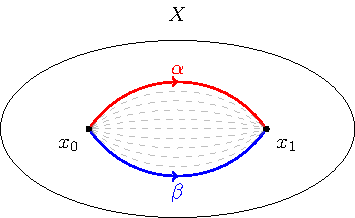
\includegraphics[]{img/homotopia-caminos}
    \end{center}
}

\rmkb{
    ¡Ojo! $F$ ahora está definida en $I\times I$, por lo que podría haber confusión al hablar de $F_t$ para $t\in I$ sin mencionar explícitamente qué componente de $F$ estamos fijando. Para nosotros, $t$ siempre será la variable de la segunda componente de $F$, y $s$ de la primera. Escribiremos $F_t(s) = F(s,t)$.
}

\propp{Relación de equivalencia $\simeq_p$}{
    $\simeq_p$ define una relación de equivalencia sobre el conjunto de caminos que unen $x_0,x_1$. Denotamos por $[\alpha]$ la clase asociada a un camino $\alpha$.
}{
    \textbf{1. Reflexiva:} $\alpha \simeq \alpha$

    Definamos la aplicación $F:I\times I \to X$ por $F(s,t) = \alpha(s)$. $F$ es continua por ser $\alpha$ continua, además se tiene
    $\begin{cases}
        F(s,0) = \alpha(s) \\
        F(s,1) = \alpha(s)
    \end{cases}$
    por lo que es una homotopía. Como además cumple
    \[
        F(0,t)=\alpha(0)=x_0, F(1,t)=\alpha(1)=x_1
    \]
    se tiene $\alpha \simeq_p \alpha$.

    \noindent\textbf{2. Simétrica:} $\alpha \simeq \beta \implies \beta \simeq \alpha$
    
    Sea $F$ la homotopía por caminos entre $\alpha, \beta$ entonces la aplicación
    \[
        \overline{F}: I \times I \to X,\quad 
        \overline{F}(s,t) = F(s,1-t)
    \]
    es una homotopía por caminos entre $\beta,\alpha$ puesto que es continua al serlo $F$ y cumple
    \[
    \overline{F}(s,0)=F(s,1)=\beta(s), \overline{F}(s,1)=F(s,0)=\alpha(s)
    \]
    así como
    \[
    \overline{F}(0,t) = F(0,1-t) = x_0, \overline{F}(1,t) = F(1,1-t) = x_1
    \]
    por tanto $\beta \simeq_p \alpha$.

    \noindent\textbf{3. Transitiva:} $\alpha \simeq \beta,\beta \simeq \gamma \implies \alpha \simeq \gamma$
    
    Sea $F_1$ la homotopía por caminos entre $\alpha,\beta$ y $F_2$ la homotopía por caminos entre $\beta,\gamma$, entonces la aplicación
    \[
    \overline{F}:I \times I \to X,\quad
    \overline{F}(s,t) =\begin{cases}
        F_1(s,2t) & t \in [0, \frac{1}{2}] \\
        F_2(s,2t-1) & t \in [\frac{1}{2}, 1]
    \end{cases}
    \]
    es continua y verifica $\overline{F}(s,0)=F_1(s,0)=\alpha(s), \overline{F}(s,1)=F_2(s,1)=\gamma(s)$, y también
    \[
        \overline{F}(0,t) = \begin{cases}
            F_1(0,2t)=x_0 & t \in [0, \frac{1}{2}] \\
            F_2(0,2t-1)=x_0 & t \in [\frac{1}{2}, 1]
        \end{cases},\quad
        \overline{F}(1,t) = \begin{cases}
            F_1(1,2t)=x_1 & t \in [0, \frac{1}{2}] \\
            F_2(1,2t-1)=x_1 & t \in [\frac{1}{2}, 1]
        \end{cases}
    \]
    por lo que es una homotopía entre $\alpha$ y $\gamma$.
}

\defn{Producto de caminos}{
    Si $\alpha$ es un camino uniendo $x_0$ y $x_1$, y $\beta$ es un camino uniendo $x_1$ y $x_2$, definimos el camino producto $\alpha * \beta$ por 
    \[
        \alpha * \beta(s) =
        \begin{cases}
            \alpha(2s) & s \in [0, \frac{1}{2}] \\
            \beta(2s - 1) & s \in [\frac{1}{2}, 1]
        \end{cases}
    \]
}

\rmkb{
    Es importante tener en mente que definimos el producto de caminos de izquierda a derecha, es decir, recorriendo primero el camino de la izquierda y después el de la derecha.
}


\lemp{Lema previo}{
    Sea $\alpha$ un camino uniendo $x_0$ y $x_1$, sea $\beta$ un camino uniendo $x_1$ y $x_2$. Entonces, para cualquier $r\in(0,1)$ se cumple $\alpha*\beta \simeq_p \gamma,\quad \gamma(t) = \begin{cases}
        \alpha(\frac{t}{r}) & t \in [0, r] \\
        \beta(\frac{t-r}{1-r}) & t \in [r, 1].
    \end{cases}$
}{
    Queremos ver que $\alpha*\beta$ y $\gamma$ son homotópicos por caminos, luego necesitamos una homotopía $H:I\times I \to X$ tal que $H(x,0) = \alpha*\beta(x)$ y $H(x,1) = \gamma(x)$, y además $H(0,t) = x_0$ y $H(1,t) = x_2$.
    
    Definamos $H$ de la siguente manera
    \[
    H(x,t) = \begin{cases}
        \alpha\Big(\frac{x}{(1-t)\frac{1}{2}+tr}\Big) & x \in [0, (1-t)\frac{1}{2}+tr] \\
        \beta\Big(\frac{x-(1-t)\frac{1}{2}-tr}{1-(1-t)\frac{1}{2}-tr}\Big) & x \in [(1-t)\frac{1}{2}+tr, 1]
    \end{cases}
    \]
    Claramente $H$ es continua por el lema del pegado y además se verifican las siguientes propiedades que necesitabamos comprobar:
    \begin{itemize}
        \item $H(x,0) = \alpha*\beta(x) \checkmark$
        \item $H(x,1) = \gamma(x) \checkmark$
        \item $H(0,t) = \alpha(0) = x_0 \checkmark$
        \item $H(1,t) = \beta(1) = x_2 \checkmark$
    \end{itemize}
}

\propp{Propiedades del producto de caminos}{
    \label{prop:propiedades-producto-caminos}
    \begin{enumerate}
        \item $\alpha * (\beta * \gamma) \simeq_p (\alpha * \beta) * \gamma$.
        \item Si $\epsilon_{x_0}$ es el arco constante $x_0$ y $\epsilon_{x_1}$ el arco constante $x_1$, entonces
        \[
            \epsilon_{x_0} * \alpha \simeq_p \alpha \text{ y } \alpha * \epsilon_{x_1} \simeq_p \alpha
        \]
        \item Sea $\bar{\alpha}(t) = \alpha(1-t), t\in I$. Entonces, $$\alpha * \bar{\alpha} \simeq_p \epsilon_{x_0} \text{ y } \bar{\alpha} * \alpha \simeq_p \epsilon_{x_1}$$
    \end{enumerate}
}{
    \begin{enumerate}
        \item Es inmediato notar que
        \begin{align*}
            \alpha * (\beta * \gamma)(s) &=
            \begin{cases}
                \alpha(2s) & s \in [0, \frac{1}{2}] \\
                \beta(4s-2) & s \in [\frac{1}{2}, \frac{3}{4}]\\
                \gamma(4s-3) & s \in [\frac{3}{4}, 1]
            \end{cases}\\
            (\alpha * \beta) * \gamma(s) &=
            \begin{cases}
                \alpha(4s) & s \in [0, \frac{1}{4}] \\
                \beta(4s-1) & s \in [\frac{1}{4}, \frac{1}{2}]\\
                \gamma(2s-1) & s \in [\frac{1}{2}, 1]
            \end{cases}
        \end{align*}
        Aplicando el lema previo con $r=\frac{1}{3}$ al primer producto obtenemos
        \[
            \alpha * (\beta * \gamma)(s) \simeq_p \sigma(s)=
            \begin{cases}
                \alpha(3s) & s \in [0, \frac{1}{3}] \\
                \beta(3s-1) & s \in [\frac{1}{3}, \frac{2}{3}]\\
                \gamma(3s-2) & s \in [\frac{2}{3}, 1]
            \end{cases}
        \]
        y de nuevo aplicandolo al segundo producto se puede llegar a $(\alpha * \beta) * \gamma(s) \simeq_p \sigma(s)$, lo que prueba finalmente que $\alpha * (\beta * \gamma) \simeq_p \sigma \simeq_p (\alpha * \beta) * \gamma$.

        \item Probaremos solo el primer caso, el segundo es muy similar. Definamos la siguiente aplicación 
        \[
        H(x,t) = \begin{cases}
            x_0 & x \in [0, \frac{t}{2}] \\
            \alpha\Big(\frac{2x-t}{2-t}\Big) & x \in [\frac{t}{2}, 1]
        \end{cases}
        \]
        que es una homotopía por caminos puesto que es continua y verifica
        \[
        H(x,1)=\epsilon_{x_0} * \alpha(x), H(x,0)=\alpha(x), H(0,t)=x_0, H(1,t)=x_1,
        \]
        luego $\alpha\simeq_p\epsilon_{x_0} * \alpha$.

        \item De nuevo probamos solo el primer caso, para ello basta definir la siguiente homotopia por caminos $H:I\times I\to X$, dada por
        \[
            H(x, t) = 
            \begin{cases} 
            \alpha(2x(1-t)) & x \in [0, \frac{1}{2}] \\
            \alpha((2-2x)(1-t)) & x \in [\frac{1}{2}, 1]
            \end{cases}
        \]
        esta aplicación es continua y efectivamente cumple $H(x,1)=\epsilon_{x_0}(x), H(0,t)=x_0, H(1,t)=x_0$, además de
        \[
        H(x,0)=
        \begin{cases} 
            \alpha(2x) & x \in [0, \frac{1}{2}] \\
            \alpha(2-2x)=\alpha(1-(2x-1))=\bar{\alpha}(2x-1) & x \in [\frac{1}{2}, 1]
            \end{cases}
        =\alpha * \bar{\alpha}(x).
        \]
    \end{enumerate}
}

\defn{Conjunto de arcos}{
    Dado $X$ un espacio topológico, denotaremos por $$\Omega_{x_0}^{x_1}(X) := \{\alpha:I\to X \text{ continua con } \alpha(0) = x_0, \alpha(1)=x_1\}$$ y $$\Omega_{x_0} = \Omega_{x_0}^{x_0}(X)$$
    Llamaremos $$\pi_1(X,x_0) : \faktor{\Omega_{x_0}}{\simeq_p}$$
}

\propp{Producto de clases de homotopía}{
    El producto $*$ induce un producto bien definido para clases de homotopía:
    $$[\alpha]*[\beta]:=[\alpha*\beta]$$
}{
    Veamos que el producto $*$ está bien definido en el cociente, es decir, no depende de los representantes elegidos de las clases $[\alpha]$ y $[\beta]$. Sean $\alpha_1, \alpha_2 \in \Omega_{x_0}^{x_1}$ con $\alpha_1 \simeq_p \alpha_2$ y $\beta_1, \beta_2 \in \Omega_{x_1}^{x_2}$ con $\beta_1 \simeq_p \beta_2$. Queremos probar que $\alpha_1 * \beta_1 \simeq_p \alpha_2 * \beta_2$. Llamemos $F_{\alpha}$ a la homotopía entre $\alpha_1$ y $\alpha_2$, y sea $F_{\beta}$ la homotopía entre $\beta_1$ y $ \beta_2$. 

    Buscamos probar que $\alpha_1 * \beta_1 $ y $\alpha_2 * \beta_2$ son caminos homotópicos. Nuestra homotopía candidata es $G : I \times I \to X$ como
    \[
        G(s, t) =
        \begin{cases}
            F_{\alpha}(2s, t) & \text{si } s \in [0, \frac{1}{2}], \\
            F_{\beta}(2s - 1, t) & \text{si } s \in [\frac{1}{2}, 1].
        \end{cases}
    \]

    Veamos que $G$ es homotopía. Es claramente continua por serlo $F_{\alpha} $ y $F_{\beta}$ y coindicir cuando $s=\frac{1}{2}$, y además verifica
    \[ 
        G(s, 0) =
        \begin{cases}
            G(s, 0) = F_{\alpha}(2s, 0) = \alpha_1(2s) = \alpha_1 * \beta_1(s) \quad & \text{si } s \in [0,\frac{1}{2}] \\
            G(s, 0) = F_{\beta}(2s - 1, 0) = \beta_1(2s) = \alpha_1 * \beta_1(s) \quad & \text{si } s \in [\frac{1}{2}, 1] 
        \end{cases}
    \]
    \[
        G(s, 1) =
        \begin{cases}
            G(s, 1) = F_{\alpha}(2s, 1) = \alpha_2(2s) = \alpha_2 * \beta_2(s) \quad & \text{si } s \in [0,\frac{1}{2}] \\
            G(s, 1) = F_{\beta}(2s - 1, 1) = \beta_2(2s) = \alpha_2 * \beta_2(s) \quad & \text{si } s \in [\frac{1}{2}, 1] 
        \end{cases}
    \] 

    Por otro lado, también se verifica la condición de homotopía de caminos, pues $\alpha_1 \simeq_p \alpha_2$ implica que $G(0, t) = F_{\alpha}(0, t) = x_0$. Análogamente, se tiene que $G(1, t) = F_{\beta}(1, t) = x_2$.

    Concluimos entonces que $\alpha_1 * \beta_1  \simeq_p \alpha_2 * \beta_2$, y por tanto $[\alpha] * [\beta]$ no depende de los representantes de las clases $[\alpha]$ y $[\beta]$.
}

Veremos a continuación que la estructura $(\pi_1(X, x_0), *)$ forma lo que en álgebra se conoce como un grupo. Un grupo es, esencialmente, un conjunto con una operación que satisface ciertas reglas (asociatividad, existencia de un elemento neutro y de inversos para cada elemento). Para una introducción más formal a los conceptos que usaremos de teoría de grupos, se puede consultar el \hyperref[apendice:teoria-de-grupos]{Apéndice A}.

\thm{El grupo fundamental}{
    El conjunto $\pi_1(X,x_0)$ junto con la operación producto $*$ es un grupo, denominado el grupo fundamental de $X$ en $x_0$.
}
\pf{
    Veamos que la operación $*$ definida en el cociente $\Omega_{x_0} / \simeq_p$ es asociativa, tiene un elemento neutro y todo elemento tiene un inverso respecto a ella. En esencia, aplicaremos la proposición \hyperref[prop:propiedades-producto-caminos]{3.3.5} a la operación en el cociente, usando que está bien definida. 
    
    \textbf{Asociatividad. } Sean $[\alpha], [\beta], [\gamma] \in \pi_1(X, x_0)$. Queremos ver que $([\alpha] * [\beta]) * [\gamma] = [\alpha] * ([\beta] * [\gamma])$. Por definición de la operación en el cociente, esto es equivalente a probar que $[(\alpha * \beta) * \gamma] = [\alpha * (\beta * \gamma)]$. La proposición \hyperref[prop:propiedades-producto-caminos]{3.3.5} (1) nos dice que $(\alpha * \beta) * \gamma \simeq_p \alpha * (\beta * \gamma)$, lo que implica que sus clases de homotopía son iguales.

    \textbf{Elemento neutro. } Sea $\epsilon_{x_0}$ el camino constante en $x_0$. La proposición \hyperref[prop:propiedades-producto-caminos]{3.3.5} (2) establece que $\epsilon_{x_0} * \alpha \simeq_p \alpha$ y $\alpha * \epsilon_{x_0} \simeq_p \alpha$ (notemos que en este caso $x_1=x_0$). En términos de clases de homotopía, esto significa que $[\epsilon_{x_0}] * [\alpha] = [\alpha]$ y $[\alpha] * [\epsilon_{x_0}] = [\alpha]$. Por lo tanto, $[\epsilon_{x_0}]$ es el elemento neutro del grupo.

    \textbf{Elemento inverso. } Para cualquier $[\alpha] \in \pi_1(X, x_0)$, consideremos el camino inverso $\bar{\alpha}(t) = \alpha(1-t)$. La proposición \hyperref[prop:propiedades-producto-caminos]{3.3.5} (3) nos dice que $\alpha * \bar{\alpha} \simeq_p \epsilon_{x_0}$ y $\bar{\alpha} * \alpha \simeq_p \epsilon_{x_0}$. Esto se traduce en $[\alpha] * [\bar{\alpha}] = [\epsilon_{x_0}]$ y $[\bar{\alpha}] * [\alpha] = [\epsilon_{x_0}]$. Por lo tanto, $[\bar{\alpha}]$ es el inverso de $[\alpha]$.

    Como la operación $*$ es asociativa, tiene elemento neutro y todo elemento tiene inverso, $(\pi_1(X, x_0), *)$ es un grupo.
}

\ex{
    Si $X\subset \R^n$ convexo, entonces $\pi_1(X,x_0) = (0,+)$ (el grupo trivial) para todo $x_0\in X$. En particular $\pi_1(\R^n,x_0) = (0,+)$ y $\pi_1(B^n, x_0) = (0,+)$, donde $B^n$ es la bola unidad.
}

\pf{
    Veamos que dado $X\subset\R^n$ convexo y $x\in X$ cualquier camino $\alpha\in\Omega_{x}$ es homotópico por caminos al camino constante $\epsilon_x$, y por tanto el grupo fundamental debe ser el grupo trivial al tener $\faktor{\Omega_{x}}{\simeq_p}$ un único elemento. Para ver que $\alpha\simeq_p\epsilon_x$ basta considerar la homotopía por caminos
    \[
    H(s,t)=t\alpha(s)+(1-t)\epsilon_x(s)=t\alpha(s)+(1-t)x
    \]
    que en efecto es continua y verifica $H(s,0)=\epsilon_x(s),H(s,1)=\alpha(s),H(0,t)=x=H(1,t)$.
}

\ex{
    $\pi_1(\R,x) = (0,+)$.
}

\rmkb{
    En los ejemplos anteriores se abusa ligeramente del lenguaje y se indica que los grupos fundamentales <<son>> el grupo trivial ya que son isomorfos a él. De hecho, cualquier grupo con un solo elemento es isomorfo al grupo trivial. Por otro lado, se suele abusar de la notación representando al grupo trivial simplemente como 0 en lugar de $(0,+)$. 
}

\defn{}{
    Sea $\sigma$ un camino uniendo dos puntos $x_0, x_1 \in X$. Definimos
    \[
    \hat{\sigma} : \pi_1(X, x_0) \to \pi_1(X, x_1)
    \]
    por
    \[
    \hat{\sigma}([\gamma]) = [\overline{\sigma}] * [\gamma] * [\sigma].
    \]
}

\propp{Proposición 6.8}{\label{prop:iso-grupos}
    La aplicación $\hat{\sigma}$ es un isomorfismo de grupos para todo camino $\sigma$. 
}{
    En primer lugar es claro que para todo $[\gamma]\in\pi_1(X,x_0)$ la imagen $\hat{\sigma}([\gamma])=[\overline{\sigma}] * [\gamma] * [\sigma] = [\overline{\sigma} * \gamma * \sigma]$ pertenece a $\pi_1(X,x_1)$, ya que
    \[
        \overline{\sigma} * \gamma * \sigma
    \]
    es un camino que parte de $x_1$ y llega a $x_1$ (recordamos que se recorre primero $\overline{\sigma}$).

    Para ver que $\hat{\sigma}$ es biyectiva comprobaremos que tiene inversa dada por
    \[
    (\hat{\sigma})^{-1}=\widehat{(\overline{\sigma})}
    \]
    en efecto se tiene
    \begin{align*}
        \widehat{(\overline{\sigma})}(\hat{\sigma}([\gamma]))=[\sigma] * \hat{\sigma}([\gamma]) * [\overline{\sigma}]=[\sigma] * [\overline{\sigma}] * [\gamma] * [\sigma] * [\overline{\sigma}] = [\gamma]
    \end{align*}
    donde hemos usado las propiedades de grupo de $\pi_1(X,x_0)$. Para comprobar que $\widehat{(\overline{\sigma})}$ también es inversa por la derecha de $\hat{\sigma}$ seguimos un razonamiento similar que omitimos.

    Para ver que es un homomorfismo basta notar que
    \begin{align*}
        \hat{\sigma}([\gamma]) * \hat{\sigma}([\alpha]) = [\overline{\sigma}] * [\gamma] * [\sigma] * [\overline{\sigma}] * [\alpha] * [\sigma] = [\overline{\sigma}] * [\gamma] * [\alpha] * [\sigma] = \hat{\sigma}([\gamma] * [\alpha])
    \end{align*}
    usando de nuevo que $\pi_1(X,x_0)$ es un grupo.
}

\rmkb{
    Podemos pensar en $\hat{\sigma}$ como un isomorfismo que cambia el <<punto base>> del grupo fundamental.
}

\corp{
    Si $X$ es conexo por caminos, todos los grupos $\pi_1(X, x_0)$ son isomorfos entre sí. En este caso, podemos considerar el grupo fundamental $\pi_1(X)$, independiente del punto base.
}{
    Sea $x_0,x_1\in X$ dos puntos arbitrarios. Entonces, existe un camino $\sigma$ que une $x_0$ y $x_1$. Por la proposición anterior se tiene que $\hat{\sigma}$ (definida segun la definición 3.3.9) es un isomorfismo de grupos, luego $\pi_1(X,x_0) \cong \pi_1(X,x_1)$.
}

\section{Espacios simplemente conexos}

\defn{Espacio simplemente conexo}{
    Decimos que un espacio topológico $X$ es simplemente conexo si es conexo por caminos y $\pi_1(X) = 0$.
}

\ex{
    Si $X \subset \mathbb{R}^n$ es convexo, entonces $X$ es simplemente conexo.
}

\clearpage

\section{El homomorfismo inducido}

\defn{Homomorfismo inducido}{
    Sea $f : X \to Y$ una aplicación continua. Para todo punto $x_0 \in X$, $f$ induce una aplicación
    \[
    f_* : \pi_1(X, x_0) \to \pi_1(Y, f(x_0))
    \]
    definida por $f_*([\alpha]) = [f \circ \alpha]$, denominada el homomorfismo inducido.
}

\clmp{}{
    $f_*$ es un homomorfismo de grupos.
}{
    En primer lugar notemos que $f\circ\alpha$ es un lazo centrado en $f(x_0)$ por ser $f$ continua. Ahora basta notar que dados $[\alpha],[\beta]\in\pi_1(X)$ tenemos
    \[
        f_*([\alpha]) * f_*([\beta]) = [f \circ \alpha] * [f \circ \beta] = [(f \circ \alpha) * (f \circ \beta)] = [f \circ (\alpha * \beta)] = f_*([\alpha * \beta]).
    \]
    Los detalles de cada paso, especialmente de
    \[
        f \circ (\alpha * \beta) = (f \circ \alpha) * (f \circ \beta)
    \]
    quedan para el lector.
}

\propp{Propiedades del homomorfismo inducido}{
    \begin{enumerate}
        \item Si $f: X \to Y$ y $g: Y \to Z$ son continuas, entonces $(g \circ f)_* = g_* \circ f_*$.
        \item Para la identidad $Id_X: X \to X$ se tiene $(Id_X)_* = Id_{\pi_1(X,x_0)}.$
        \item Si $f$ es un homeomorfismo, entonces $f_*$ es un isomorfismo de grupos. Así, el grupo fundamental es un invariante topológico.
    \end{enumerate}
}{
    \begin{enumerate}
        \item Sea $[\alpha]\in\pi_1(X)$, entonces
        \[
            (g \circ f)_*([\alpha])=[(g\circ f)\circ \alpha] = [g\circ(f\circ\alpha)] = g_*([f\circ\alpha]) = g_*(f_*([\alpha])) = g_* \circ f_* ([\alpha]).
        \]
        \item Es inmediato verificar que
        \[
            (Id_X)_*([\alpha]) = [Id_X \circ \alpha] = [\alpha] = Id_{\pi_1(X,x_0)}([\alpha])
        \]
        \item Ya sabemos que $f_*$ es un homomorfismo. Para ver que es una biyección notemos que $f^{-1}$ también es continua por ser $f$ homeomorfismo, por tanto, usando los apartados anteriores
        \begin{align*}
            f^{-1}_* \circ f_* &= (f^{-1} \circ f)_* = (Id_X)_* = Id_{\pi_1(X,x_0)}\\
            f_* \circ f^{-1}_* &= (f \circ f^{-1})_* = (Id_X)_* = Id_{\pi_1(Y,f(x_0))} 
        \end{align*}
        luego $f^{-1}_*$ es la inversa de $f_*$ y por tanto es una biyección.
    \end{enumerate}
}

\lem{}{
    Sea $X$ un espacio topológico y sean $\sigma_1$ y $\sigma_2$ arcos homotópicos en $X$ (no necesariamente por caminos). Entonces existen arcos $\tau_1$ uniendo $\sigma_1(0)$ con $\sigma_2(0)$ y $\tau_2$ uniendo $\sigma_1(1)$ con $\sigma_2(1)$ tales que
    \[
        \sigma_2 \simeq_p \overline{\tau}_1 * \sigma_1 * \tau_2.
    \]
    De hecho, si $\sigma_i$ es un lazo centrado en $x_i\in X$, $i=1,2$, entonces pueden elegirse $\tau_2=\overline{\tau}_1$.
}

\pf{
    \textit{Esquema de la prueba}

    Como $\sigma_1 \simeq \sigma_2$ existe una homotopía $F:I\times I\to X$ tal que $F(x,0)=\sigma_1(x),F(x,1)=\sigma_2(x)$. Entonces basta tomar $\tau_1(t)=F(0,t),\tau_2(t)=F(1,t)$ y vemos que $\sigma_2$ y $\overline{\tau}_1 * \sigma_1 * \tau_2$ son homotópicos por caminos.
}

\propp{}{
    Sean \( X \) e \( Y \) espacios topológicos, \( x_0 \in X \) y \( F \) una homotopía entre las aplicaciones continuas \( f, g : X \to Y \). Si denotamos por  
    \[
        \sigma(t) := F(x_0, t), \quad t \in I \text{ entonces } \hat{\sigma} \circ f_{*} = g_{*},
    \]  
    es decir, el siguiente diagrama es conmutativo:  
    \begin{center}
        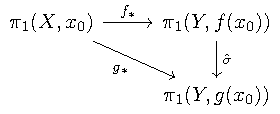
\includegraphics[]{otros/diagrama-prop-6-11.pdf}
    \end{center}
}{
    Sea $[\alpha]\in\pi_1(X,x_0)$, notemos en primer lugar que $f\circ\alpha,g\circ\alpha$ son lazos en torno al mismo punto. Además sabemos que
    \begin{align*}
        \hat{\sigma} \circ f_{*}([\alpha]) = g_*([\alpha]) \iff  [\overline{\sigma}] * [f \circ \alpha] * [\sigma]  = [g \circ \alpha] \iff \\
        \iff [f \circ \alpha] = [\sigma] * [g \circ \alpha] * [\overline{\sigma}] \iff [f \circ \alpha] = [\sigma * g \circ \alpha * \overline{\sigma}]
    \end{align*}
    por tanto solo hace falta ver que
    \[
    \sigma * g \circ \alpha * \overline{\sigma} \simeq_p f \circ \alpha.
    \]
    Para probar esto último consideremos la homotopía por caminos siguiente
    \[
    G(s,t)=\begin{cases}
        \sigma(3ts) = F(x_0,3ts) & s\in[0,\frac{1}{3}]\\
        F(\alpha(3s-1),t) & s\in[\frac{1}{3},\frac{2}{3}]\\
        \sigma(3t(1-s))F(x_0,3t(1-s)) & s\in[\frac{2}{3},1]
    \end{cases}
    \]
    ahora basta notar que $G(s,0)$ es una reparametrización del producto de caminos $\epsilon_{f(x_0)} * (f\circ\alpha) * \epsilon_{f(x_0)}$ mientras que $G(s,1)$ es una reparametrización del producto de caminos $\sigma * (g\circ\alpha) * \overline{\sigma}$, lo que nos permite afirmar que $\epsilon_{f(x_0)} * (f\circ\alpha) * \epsilon_{f(x_0)} \simeq_p \sigma * (g\circ\alpha) * \overline{\sigma}$.

    Finalmente aplicando la \hyperref[prop:propiedades-producto-caminos]{Proposición 3.3.5} obtenemos 
    \[
        f\circ\alpha \simeq_p \epsilon_{f(x_0)} * f\circ\alpha * \epsilon_{f(x_0)} \simeq_p \sigma * g\circ\alpha * \overline{\sigma}
    \]
    como queríamos ver.
}

\corp{
    El grupo fundamental es un invariante homotópico. En efecto, si  
    \[
        f : X \to Y
    \]  
    es una equivalencia de homotopía entre espacios topológicos homotópicamente equivalentes, entonces  
    \[
        f_{*} : \pi_1(X, x_0) \to \pi_1(Y, f(x_0))
    \]  
    es un isomorfismo de grupos.
}{
    Por ser $f$ una equivalencia de homotopía debe existir $g$ tal que
    \[
        g \circ f \simeq Id_X, \quad f \circ g \simeq Id_Y
    \]
    Sea $F_X$ la homotopía entre $Id_X,g \circ f$ y sea $F_Y$ la homotopía entre $Id_Y, f \circ g$. Sea $x_0 \in X$ y sea  $\sigma_X=F_X(x_0,t)$ aplicando la proposición anterior obtenemos:
    \begin{align*}
        \hat{\sigma}_X \circ (Id_X)_* = \hat{\sigma}_X \circ Id_{\pi_1(X,x_0)} = g_* \circ f_*
    \end{align*}
    Como $\hat{\sigma}_X, Id_{\pi_1(X,x_0)}$ son isomorfismos su composición también lo es, por tanto $g_* \circ f_*$ es un isomorfismo, lo que implica que $f_*$ debe ser inyectiva. 
    
    Similarmente, consideremos la aplicación $\sigma_Y=F_Y(f(x_0),t)$, aplicando la proposición anterior obtenemos:
    \begin{align*}
        \hat{\sigma}_Y \circ (Id_Y)_* = \hat{\sigma}_Y \circ Id_{\pi_1(Y,f(x_0))} = f_* \circ g_*
    \end{align*}
    igual que antes $\hat{\sigma}_X \circ Id_{\pi_1(Y,f(x_0))}$ es un isomorfismo, y por tanto $f_*$ debe ser sobreyectiva, lo que finaliza la prueba puesto que ya sabemos que es un homomorfismo. 
}

\corp{
    Si $X$ es un espacio contráctil entonces $X$ es simplemente conexo.
}{
    Si $X$ es contráctil entonces es homotópico a un punto $\{x\}$, como el único lazo en este espacio es el lazo constante, su grupo fundamental es el grupo trivial: $\pi_1(\{x\})\cong(0,+)$. Finalmente, por el corolario anterior el grupo fundamental es un invariante homotópico, y como $X\simeq\{x\}$ hemos de tener
    \[
    \pi_1(X)\cong\pi_1(\{x\})\cong(0,+).
    \]
    Finalmente, el \hyperref[cor:contractil-arcoconexo]{Corolario 3.2.3} nos permite asegurar que $X$ es arcoconexo, lo que prueba que $X$ es simplemente conexo.
}

\clearpage

\section{Aplicaciones recubridoras}

\defn{Aplicación recubridora}{
    Sea $p:E \to B$ una aplicación continua y sobreyectiva. Decimos que $p$ es una aplicación recubridora si para todo $b \in B$ existe un entorno $U\in\E(b)$ tal que
    \[
        p^{-1}(U)=\bigcup_{i \in J} V_i
    \]
    donde los $V_i$ son abiertos disjuntos en $E$ y
    \[
    p|_{V_i}:V_i \to U
    \]
    es un homeomorfismo para todo $i \in J$.
    Se dice que $E$ es un espacio recubridor de $B$. Si $J=\{1,\dots,n\}$ diremos que $p$ es una aplicación recubridora de $n$ hojas.
}

\ex{
    La aplicación $p : \mathbb{R} \to \mathbb{S}^1$ dada por $p(t) = (\cos 2\pi t, \sin 2\pi t)$ es una aplicación recubridora.
}

\pf{
    $p$ es continua por ser composición de funciones continuas, y es sobreyectiva pues todo punto en $\mathbb{S}^1$ puede expresarse en coordenadas polares como $(\cos \theta, \sin \theta)$ para algún $\theta \in \mathbb{R}$, luego $p(\frac{\theta}{2\pi})=b$.

    Sea $b = (\cos \theta, \sin \theta) \in \mathbb{S}^1$. Tomemos el entorno $U = \mathbb{S}^1 \setminus \{-b\}$, entonces
    \[
    p^{-1}(U) = \bigcup_{k \in \mathbb{Z}} \left( k + \frac{\theta}{2\pi} - \frac{1}{2}, k + \frac{\theta}{2\pi} + \frac{1}{2} \right),
    \]
    donde cada $V_k = \left( k + \frac{\theta}{2\pi} - \frac{1}{2}, k + \frac{\theta}{2\pi} + \frac{1}{2} \right)$ es abierto en $\mathbb{R}$ y $p|_{V_k} \colon V_k \to U$ es un homeomorfismo. Los $V_k$ son disjuntos y $p$ restringida a cada $V_k$ es biyectiva, con inversa continua.
}

\ex{
    La aplicación $p : \mathbb{S}^1 \to \mathbb{S}^1$ dada por $p(x, y) = (x^2 - y^2, 2xy)$ (elevar al cuadrado en $\mathbb{C}$) es una aplicación recubridora.
}

\pf{
    $p$ es continua por serlo cada componente, y es sobreyectiva pues dado $b = (\cos \theta, \sin \theta) \in \sphere^1, \theta \in \R$ podemos tomar $(x,y)=(\cos \frac{\theta}{2}, \sin \frac{\theta}{2})$ de manera que
    \[
    p(x,y)=(\cos \frac{\theta}{2} - \sin \frac{\theta}{2}, 2\cos \frac{\theta}{2}\sin \frac{\theta}{2})=(\cos \theta, \sin \theta) = b.
    \]
    
    Además, para cualquier $b \in \mathbb{S}^1$, podemos tomar $U = \mathbb{S}^1 \setminus \{-b\}$. Supongamos ahora que el punto $b$ está en el primer cuadrante, para el resto de cuadrantes podemos razonar de manera similar. Es fácil comprobar que
    \[
    p^{-1}(-b)=\{a,b\},\quad a=(\cos(\theta+\frac{\pi}{2}),\sin(\theta+\frac{\pi}{2})), b=(\cos(\theta+\frac{3\pi}{2}),\sin(\theta+\frac{3\pi}{2}))
    \]
    Entonces es claro que:
    \[
        p^{-1}(U) = V_1 \cup V_2,
    \]
    donde $V_1$ y $V_2$ son los dos hemisferios abiertos de $\mathbb{S}^1$ dados por
    \[
    V_1=\{(\cos\alpha,\sin\alpha) \mid \alpha \in (\theta+\frac{\pi}{2},\theta+\frac{3\pi}{2})\},\quad V_2=\{(\cos\alpha,\sin\alpha) \mid \alpha \in (\theta+\frac{3\pi}{2},2\pi)\cup[0,\theta+\frac{\pi}{2})\}.
    \]
    Cada $V_i$ es un "sector" de $\mathbb{S}^1$ que cubre la mitad del círculo, y $p|_{V_i}$ es un homeomorfismo. Si $b$ no estuviera en el primer cuadrante también obtenemos dos hemisferios abiertos, los detalles se dejan como ejercicio.
}

\propp{}{
    El producto de dos aplicaciones recubridoras es una aplicación recubridora.
}{
    Sean $p_1 \colon E_1 \to B_1$ y $p_2 \colon E_2 \to B_2$ aplicaciones recubridoras. Entonces el producto es
    \[
    p = p_1 \times p_2 \colon E_1 \times E_2 \to B_1 \times B_2, \quad p(e_1, e_2)=(p_1(e_1), p_2(e_2)).
    \]
    Para ver que $p$ es una aplicación recubridora es inmediato que
    $p$ es continua y sobreyectiva porque $p_1$ y $p_2$ lo son.

    Dado $(b_1, b_2) \in B_1 \times B_2$, existen entornos $U_1 \subset B_1$ de $b_1$ y $U_2 \subset B_2$ de $b_2$ tales que:
    \[
    p_1^{-1}(U_1) = \bigcup_{i \in I} V_i^1, \quad p_2^{-1}(U_2) = \bigcup_{j \in J} V_j^2,
    \]
    con los $V_i^1, V_j^2$ disjuntos y tales que $p_1|_{V_i^1} \colon V_i^1 \to U_1$ y $p_2|_{V_j^2} : V_j^2 \to U_2$ son homeomorfismos. Entonces, para $U = U_1 \times U_2$, tenemos:
    \[
    p^{-1}(U) = \bigcup_{(i,j) \in I \times J} V_i^1 \times V_j^2.
    \]
    Cada $V_i^1 \times V_j^2$ es abierto en $E_1 \times E_2$, son disjuntos, y:
    \[
        p|_{V_i^1 \times V_j^2} \colon V_i^1 \times V_j^2 \to U_1 \times U_2
    \]
    es un homeomorfismo porque es producto de homeomorfismos. Por lo tanto, $p_1 \times p_2$ es una aplicación recubridora.
}

\ex{
    Sea $p : \mathbb{R} \to \mathbb{S}^1$ dada por $p(t) = (\cos 2\pi t, \sin 2\pi t)$, entonces $p \times p : \mathbb{R}^2 \to \mathbb{S}^1 \times \mathbb{S}^1$ es una aplicación recubridora sobre el toro.
}

% Faltan las demostraciones de los dos lemas. Están en la clase del 29/04

\lem{Levantamiento de caminos}{
    Sea $p : E \to B$ una aplicación recubridora. Sean $e \in E$, $b \in B$ tales que $p(e) = b$. Para cualquier camino $\alpha : I \to B$ que comienza en $b$, existe un único camino $\tilde{\alpha} : I \to E$ que comienza en $e$ tal que $p \circ \tilde{\alpha} = \alpha$. El camino $\tilde{\alpha}$ se llama levantamiento de $\alpha$.
}

\lem{Levantamiento de homotopías}{
    Sea $p : E \to B$ una aplicación recubridora. Sean $e \in E$, $b \in B$ tales que $p(e) = b$. Para cualquier homotopía por caminos $F : I \times I \to B$ con $F(0,0) = b$, existe una única homotopía por caminos $\tilde{F} : I \times I \to E$ tal que $p \circ \tilde{F} = F$ y $\tilde{F}(0,0) = e$.
}

\propp{}{
    Sea $p : E \to B$ una aplicación recubridora. Sean $e \in E$, $b \in B$ tales que $p(e) = b$. Sean $\alpha$, $\beta$ dos caminos en $B$ comenzando en $b$ y finalizando en un mismo punto $b'$, y sean $\tilde{\alpha}$, $\tilde{\beta}$ sus respectivos levantamientos comenzando en $e$. Si $\alpha \simeq_p \beta$, entonces $\tilde{\alpha} \simeq_p \tilde{\beta}$ y $\tilde{\alpha}$, $\tilde{\beta}$ finalizan en un mismo punto de $E$.
}{
    Supongamos que $\alpha \simeq_p \beta$ y sea $F$ la homotopía por caminos entre $\alpha,\beta$, con $F(0,0)=b$. Por el lema anterior existe una única homotopía por caminos $\tilde{F}$, que cumple $\tilde{F}(0,t)=e,\tilde{F}(1,t)=e'$ para un cierto $e'$. Veamos que es una homotopía entre $\tilde{\alpha},\tilde{\beta}$, en efecto
    \begin{align*}
        p\circ\tilde{F}(s,0)=F(s,0)=\alpha(s)\implies \tilde{F}(s,0)=\tilde{\alpha}(s)\\
        p\circ\tilde{F}(s,1)=F(s,1)=\beta(s)\implies \tilde{F}(s,1)=\tilde{\beta}(s)
    \end{align*}
    y como además mantiene fijos los extremos es una homotopía de caminos, por tanto $\tilde{\alpha}\simeq_p\tilde{\beta}$.
}

\defn{Correspondencia del levantamiento}{
    Sea $p : E \to B$ una aplicación recubridora. Sean $e \in E$, $b \in B$ tales que $p(e) = b$. Definimos la aplicación
    \[
    \Phi : \pi_1(B, b) \to p^{-1}(b)
    \]
    que asigna a cada clase de lazos $[\alpha] \in \pi_1(B, b)$ un elemento de $E$. En concreto, sea $\tilde{\alpha}$ el levantamiento de $\alpha$ que empieza en $e$, entonces ese elemento es
    \[
    \Phi([\alpha]) := \tilde{\alpha}(1).
    \]
}

\propp{}{
    Sea $p : E \to B$ una aplicación recubridora. Sean $e \in E$, $b \in B$ tales que $p(e) = b$.
    \begin{enumerate}
        \item Si $E$ es conexo por caminos, entonces $\Phi$ es sobreyectiva.
        \item Si $E$ es simplemente conexo, entonces $\Phi$ es biyectiva.
    \end{enumerate}
}{
    \begin{enumerate}
        \item Si $E$ es conexo por caminos dado $e' \in p^{-1}(b)$ existe un camino $\tilde{\alpha}$ en $E$ uniendo $e$ con $e'$. Entonces $\alpha=p\circ\tilde{\alpha}$ es un lazo centrado en $b$ con $\Phi([\alpha])=\alpha(1)=e'$ por definición, luego $\Phi$ es sobreyectiva.
        \item Si $E$ es simplemente conexo entonces es conexo por caminos, por lo que el apartado anterior garantiza la sobreyectividad.
        
        Para ver que es inyectiva sean $[\alpha],[\beta]\in\pi_1(B,b)$ tales que $\Phi([\alpha])=\Phi([\beta])$. Sean $\tilde{\alpha},\tilde{\beta}$ los levantamientos empezando en $e$ y terminando en $\tilde{\alpha}(1)=\tilde{\beta}(1)$ dados por la proposición anterior. Como $E$ es simplemente conexo existe una homotopía por caminos $\tilde{F}$ entre $\tilde{\alpha},\tilde{\beta}$, pero entonces $F=p\circ\tilde{F}$ es una homotopía por caminos entre $\alpha,\beta$, por lo que $[\alpha]=[\beta]$.
    \end{enumerate}
}

\thm{}{
    El grupo fundamental de la circunferencia $\mathbb{S}^1$ es isomorfo a $(\mathbb{Z}, +)$.
}

\pf{
    Sea $p:\R \to \sphere^1$ dada por $p(t)=(\cos(2\pi t), \sin(2\pi t))$ y sea $e=0, b=p(0)=(1,0)$. Como ya sabemos, $p$ es una aplicación recubridora. Además, $p^{-1}(b)=\mathbb{Z}$, y como $\R$ es simplemente conexo la aplicación $\Phi$ es una biyección. Veamos que también es un homomorfismo.

    Sean $[\alpha],[\beta]\in\pi_1(\sphere^1,b)$ y sean $\tilde{\alpha},\tilde{\beta}$ los levantamientos empezando en $e$ y terminando en $\tilde{\alpha}(1)=n, \tilde{\beta}(1)=m,\quad n,m\in\mathbb{Z}$. Consideremos el camino en $\R$ dado por
    \[
    \tilde{\tilde{\beta}}:I\to\R, \tilde{\tilde{\beta}}(s)=n+\tilde{\beta}(s)
    \]
    como $p(x+n)=p(x)$ para todo $x\in\R$ entonces $\tilde{\tilde{\beta}}$ es un levantamiento de $\beta$ que comienza en $\tilde{\tilde{\beta}}(0)=n$ en lugar de en $0$. Entonces $\tilde{\alpha}*\tilde{\tilde{\beta}}$ está bien definido ya que
    \[
        \tilde{\alpha}(1)=n=\tilde{\tilde{\beta}}(0)
    \]
    y es un levantamiento de $\alpha*\beta$ que comienza en $0$. Notemos ahora que el punto final de $\tilde{\alpha}*\tilde{\tilde{\beta}}$ es $\tilde{\tilde{\beta}}(1)=n+m$, luego tenemos
    \[
        \Phi([\alpha*\beta])=n+m=\tilde{\alpha}(1)+\tilde{\beta}(1)=\Phi([\alpha])+\Phi([\beta])
    \]
    lo que prueba que $\Phi$ es un homomorfismo.
}

\clearpage
\section{Retractos}

\defn{Retracción, retracto}{
    Sea $A \subset X$ un subconjunto de un espacio topológico $X$. Una retracción de $X$ en $A$ es una aplicación continua $r : X \to A$ tal que $r|_A = Id_A$. Se dice que $A$ es un retracto de $X$.
}

\ex{
    La aplicación $r : \mathbb{R}^{n+1} \setminus \{0\} \to \mathbb{S}^n$ dada por $r(x) = \frac{x}{\|x\|}$ es una retracción, así $\mathbb{S}^n$ es un retracto de $\mathbb{R}^{n+1} \setminus \{0\}$.
}

\lem{}{
    Si $A$ es un retracto de $X$, entonces el homomorfismo inducido $i_* : \pi_1(A, a) \to \pi_1(X, a)$ es inyectivo, para todo $a \in A$, donde $i : A \to X$ es la inclusión.
}

\pf{
    Sea $r$ la retracción de $X$ en $A$. Sean $[\alpha]_A,[\beta]_A\in\pi_1(A, a)$, entonces
    \[
        i_*([\alpha]_A)=i_*([\beta]_A) \implies [i\circ\alpha]_X=[i\circ\beta]_X \implies [\alpha]_X=[\beta]_X.
    \]
    Como $[\alpha]_X=[\beta]_X$ existe una homotopía por caminos $F:I\times I\to X$ entre $\alpha$ y $\beta$. Sea entonces $\tilde{F}:I\times I \to A, \tilde{F} = r \circ F$, que está bien definida porque las imágenes de $\alpha,\beta$ están en $A$. Además $\tilde{F}$ es una homotopía por caminos, luego $[\alpha]_A = [\beta]_A$.
}

\defn{Retracto de deformación}{
    Sea $A \subset X$ un retracto de $X$. Decimos que $A$ es un retracto de deformación de $X$ si la aplicación identidad $Id_X$ es homotópica a $i \circ r$, con $r$ una retracción de $X$ en $A$, de forma que cada punto de $A$ permanece fijo por la homotopía. En particular, $A \simeq X$.
}

\ex{
    $\mathbb{S}^n$ es un retracto de deformación de $\mathbb{R}^{n+1} \setminus \{0\}$.
}

% Falta ver que $r(x) = \frac{x}{\|x\|}$ es homotópica a lo otro 

\corp{
    Sea $A$ un retracto de deformación de $X$. Para todo $a \in A$, el homomorfismo inducido $i_* : \pi_1(A, a) \to \pi_1(X, a)$ por la inclusión es un isomorfismo.
}{
    Como $A$ es un retracto de deformación de $X$ sabemos que $i \circ r \simeq Id_X$, y además es inmediato que $r \circ i = Id_A$. Veamos que $i_*$ es sobreyectiva y habremos terminado, puesto que ya sabemos que es un homomorfismo y que es inyectiva.

    Sea $[\alpha]_X \in \pi_1(X, a)$ y sea
    \[
        \tilde{\alpha}:I\to A,\quad \tilde{\alpha}(s)=r(\alpha(s))
    \]
    entonces
    \[
        i_*([\tilde{\alpha}]_A)=[i\circ\tilde{\alpha}]_X=[(i\circ r)\circ \alpha]_X=[\alpha]_X
    \]
    donde la última igualdad se da porque $i \circ r \simeq Id_X$, luego $i \circ r \circ \alpha \simeq Id_X \circ \alpha \simeq \alpha$.
}

\corp{
    $\pi_1(\mathbb{R}^{n+1} \setminus \{0\}) \cong \pi_1(\mathbb{S}^n)$, para todo $n \geq 1$.
}{
    Por el ejemplo anterior $\sphere^n$ es un retracto de deformación de $\mathbb{R}^{n+1} \setminus \{0\}$, luego $i_*$ es el isomorfismo buscado entre $\pi_1(\mathbb{R}^{n+1} \setminus \{0\})$ y $\pi_1(\mathbb{S}^n)$.
}

\clearpage

\section{Teorema de Seifert-van Kampen}

\thm{Teorema de Seifert-van Kampen (versión reducida)}{
    Supongamos que $X = U \cup V$, donde $U$ y $V$ son abiertos y $U \cap V \neq \emptyset$ es conexo por caminos. Sean $i : U \to X$ y $j : V \to X$ las inclusiones. Para cada $x_0 \in U \cap V$, las imágenes de los homomorfismos inducidos $i_*$ y $j_*$ generan el grupo $\pi_1(X, x_0)$.
}

\pf{
    Queremos ver que dado $[\alpha]\in\pi_1(X, x_0)$ se tiene que 
    \[
        [\alpha]=[\beta_1 * \dots * \beta_n]
    \]
    con cada $\beta_k$ contenido en $U$ o en $V$.

    Existe una subdivisión de $[0,1]$ de la forma $0=a_0<a_1<\dots<a_n=1$ tal que $\alpha(a_i)\in U \cap V$ y $\alpha([a_{i-1},a_{i}])$ está contenido en $U$ o en $V$.

    Definamos $\alpha_i$ como un camino que cubre el trozo de $\alpha$ en el intervalo $[a_{i-1},a_{i}]$ haciendo
    \[
    \alpha_i(t)=\alpha(a_{i-1}+t(a_{i}-a_{i-1})).
    \]
    Es inmediato entonces que 
    \[
    \alpha \simeq_p \alpha_1 * \dots * \alpha_n.
    \]
    Cada curva $\alpha_i$ es un camino uniendo puntos de $U\cap V$, que es conexo por caminos. Por tanto, existe $\gamma_i$ un camino contenido en $U\cap V$ uniendo $x_0$ con $\alpha(a_i)$ . Como $\alpha(a_0)=x_0=\alpha(a_n)$, los arcos $\gamma_1,\gamma_n$ son constantes.

    Finalmente, definamos los arcos $\beta_i=\gamma_{i-1} * \alpha_i * \overline{\gamma_i}$, entonces se tiene que $\beta_i$ es un lazo en $x_0$ y además
    \[
        \beta_1 * \beta_2 * \dots * \beta_n \simeq_p \alpha_1 * \dots * \alpha_n \simeq_p \alpha
    \]
    lo que nos permite concluir 
    \[
        [\alpha]=[\beta_1 * \dots * \beta_n]
    \]
    como queríamos ver.
}

\rmkb{
    Es fácil visualizar el teorema en el caso de los lazos simples. Si tomamos un punto $x_0 \in U\cap V$ y un lazo simple $\alpha$ centrado en $x_0$, entonces siempre podemos dividir este camino en dos lazos distintos $\alpha_1,\alpha_2$ de manera que $\alpha_1$ está en $U$ y $\alpha_2$ está en $V$, y además $[\alpha]=[\alpha_1 * \alpha_2].$
}

\corp{
    Supongamos que $X = U \cup V$, donde $U$ y $V$ son abiertos y $U \cap V \neq \emptyset$, $U$ y $V$ son conexos por caminos. Si $U$ y $V$ son simplemente conexos, entonces $X$ es simplemente conexo.
}{
    Como $U,V,U \cup V$ son conexos por caminos, $X$ lo es, y por tanto $\pi_1(X)\cong\pi_1(X,x_0)$ para cualquier $x_0\in U\cup V$. Por el Teorema de Seifert-van Kampen $\pi_1(X,x_0)$ está generado por $i_*,j_*$, pero al ser $U,V$ simplemente conexos esto quiere decir que $\pi_1(X,x_0)$ es isomorfo al grupo trivial, por tanto $X$ es simplemente conexo.
}

\corp{
    La esfera $\mathbb{S}^n$ es simplemente conexa para $n \geq 2$.
}{
    Sean $p=(0,\dots,1)\in\R^{n+1}$ y $q=(0,\dots,-1)\in\R^{n+1}$, entonces $\sphere^n\setminus\{p\}$ es homeomorfa a $\R^n$, por tanto simplemente conexa. De igual manera, $\sphere^n\setminus\{q\}$ es homeomorfa a $\R^n$ y por tanto simplemente conexa. Finalmente notemos que
    \[
    \left( \sphere^n\setminus\{p\} \right) \cap \left( \sphere^n\setminus\{q\} \right) \neq \emptyset, \left( \sphere^n\setminus\{p\} \right) \cup \left( \sphere^n\setminus\{q\}\right) = \sphere^n
    \]
    por tanto, por el corolario anterior, $\sphere^n$ es simplemente conexa.
}

\thm{}{
    Sean $X$ e $Y$ dos espacios topológicos y fijemos puntos $x_0 \in X$, $y_0 \in Y$. Entonces
    \[
    \pi_1(X \times Y, (x_0, y_0)) \cong \pi_1(X, x_0) \times \pi_1(Y, y_0).
    \]
}
\pf{
    Queremos construir un isomorfismo de grupos
    \[
        \Phi : \pi_1(X \times Y, (x_0, y_0)) \longrightarrow \pi_1(X, x_0) \times \pi_1(Y, y_0).
    \]
    Consideremos las proyecciones canónicas $p : X \times Y \to X$ y $q : X \times Y \to Y$. Estas aplicaciones son continuas y, por lo tanto, inducen homomorfismos entre los grupos fundamentales:
    \begin{align*}
        p_* &: \pi_1(X \times Y, (x_0, y_0)) \longrightarrow \pi_1(X, x_0) \\
        q_* &: \pi_1(X \times Y, (x_0, y_0)) \longrightarrow \pi_1(Y, y_0).
    \end{align*}
    Definimos la aplicación $\Phi$ de la siguiente manera: para cualquier lazo $[\alpha] \in \pi_1(X \times Y, (x_0, y_0))$,
    \[
        \Phi([\alpha]) := (p_*([\alpha]), q_*([\alpha])) = ([p \circ \alpha]_X, [q \circ \alpha]_Y).
    \]
    Para demostrar que $\Phi$ es un isomorfismo, verificaremos que es un homomorfismo y que es biyectiva.

    \paragraph{1. $\Phi$ es un homomorfismo}
    Sean $[\alpha], [\beta] \in \pi_1(X \times Y, (x_0, y_0))$. Entonces,
    \begin{align*}
        \Phi([\alpha] * [\beta]) &= \Phi([\alpha * \beta]) \\
        &= (p_*([\alpha * \beta]), q_*([\alpha * \beta])) \\
        &= ([p \circ (\alpha * \beta)]_X, [q \circ (\alpha * \beta)]_Y).
    \end{align*}
    Dado que $[p \circ (\alpha * \beta)]_X = [p \circ \alpha]_X * [p \circ \beta]_X$ y análogamente $[q \circ (\alpha * \beta)]_Y = [q \circ \alpha]_Y * [q \circ \beta]_Y$, se sigue que
    \begin{align*}
        p_*([\alpha * \beta]) &= [p \circ \alpha * p \circ \beta]_X = [p \circ \alpha]_X * [p \circ \beta]_X = p_*([\alpha]) * p_*([\beta]) \\
        q_*([\alpha * \beta]) &= [q \circ \alpha * q \circ \beta]_Y = [q \circ \alpha]_Y * [q \circ \beta]_Y = q_*([\alpha]) * q_*([\beta]).
    \end{align*}
    Por lo tanto,
    \begin{align*}
        \Phi([\alpha] * [\beta]) &= (p_*([\alpha]) * p_*([\beta]), q_*([\alpha]) * q_*([\beta])) \\
        &= (p_*([\alpha]), q_*([\alpha])) * (p_*([\beta]), q_*([\beta])) \\
        &= \Phi([\alpha]) * \Phi([\beta]).
    \end{align*}
    Así, $\Phi$ es un homomorfismo de grupos.

    \paragraph{2. $\Phi$ es inyectiva}
    Sabemos que un homomorfismo es inyectivo si y solo si su núcleo es trivial. En este caso, el núcleo de $\Phi$ está dado por
    \[
        Ker(\Phi) = \{[\alpha] \in \pi_1(X \times Y, (x_0, y_0)) : [p \circ \alpha] = [\varepsilon_{x_0}], [q \circ \alpha] = [\varepsilon_{y_0}]\}.  
    \]

    Supongamos que $\alpha$ es un lazo en $(x_0, y_0)$ con $[\alpha] \in Ker(\Phi)$. Esto implica que $p \circ \alpha \simeq_p \varepsilon_{x_0}$ y $q \circ \alpha \simeq_q \varepsilon_{y_0}$. Sean $H$ y $G$ las respectivas homotopías. Entonces, definimos

    \[
        F((x, y), t) = (H(x, t), G(y, t)),
    \]
    que es homotopía entre $\alpha$ y el lazo constante en $(x_0, y_0)$. Por lo tanto, $[\alpha] = [\varepsilon_{(x_0, y_0)}]$, lo que implica que el núcleo de $\Phi$ es trivial.
    \paragraph{3. $\Phi$ es sobreyectiva}
    Sea $\gamma_1$ lazo en $X$ centrado en $x_0$ y $\gamma_2$ lazo en $Y$ centrado en $y_0$. Buscamos $[\alpha] \in \pi_1(X \times Y, (x_0, y_0))$ tal que $\Phi([\alpha]) = ([\gamma_1], [\gamma_2])$. 

    Basta tomar $\alpha(s) = (\gamma_1(s), \gamma_2(s))$ para $s \in [0, 1]$ y observar que cumple las condiciones. 

    \vspace{0.5cm}
    Hemos visto que $\Phi$ es un homomorfismo de grupos, inyectivo y sobreyectivo, por lo que es un isomorfismo. 
}   

\corp{
    $\pi_1(\mathbb{S}^1 \times \mathbb{S}^1) \cong \mathbb{Z} \times \mathbb{Z}$.
}{
    Pendiente.
}

\propp{}{
    El grupo fundamental del plano proyectivo $\mathbb{RP}^2$ es $\mathbb{Z}_2$.
}{
    Pendiente.
}

\propp{}{
    El grupo fundamental de la figura ocho $\mathbb{S}^1 \lor \mathbb{S}^1$ es no abeliano (grupo libre de dos generadores).
}{
    Pendiente.
}

\corp{
    El grupo fundamental del plano doblemente agujereado es no abeliano.
}{
    Pendiente.
}

\corp{
    El grupo fundamental del doble toro $\mathbb{T}^2 \#\mathbb{T}^2$ es no abeliano.
}{
    Pendiente.
}

% % chapter1.tex
\chapter{Examples}

\section{Theorem System}

\defn{Definition Name}{
    A definition.
}

\thmr{Theorem Name}{mybigthm}{
    A theorem.
}

\lem{Lemma Name}{
    A lemma.
}

\fact{
    A fact.
}

\cor{
    A corollary.
}

\prop{}{
    A proposition.
}

\exer{
    Exercise example.
}

\clmp{}{
    A claim.
}{
    A reference to Theorem~\ref{thm:mybigthm}
}

\pf{
    Veniam velit incididunt deserunt est proident consectetur non velit ipsum voluptate nulla quis. Ea ullamco consequat non ad amet cupidatat cupidatat aliquip tempor sint ea nisi elit dolore dolore. 

    Laboris labore magna dolore eiusmod ea ex et eiusmod laboris. Et aliquip cupidatat reprehenderit id officia pariatur. 
}

\ex{
    Nostrud esse occaecat Lorem dolore laborum exercitation adipisicing eu sint sunt et. Excepteur voluptate consectetur qui ex amet esse sunt ut nostrud qui proident non. Ipsum nostrud ut elit dolor. Incididunt voluptate esse et est labore cillum proident duis.
}



\rmk{
    Some remark.
}

\rmkb{
    Some more remark.
}

\section{Pictures}

\begin{figure}[H]
    \center
    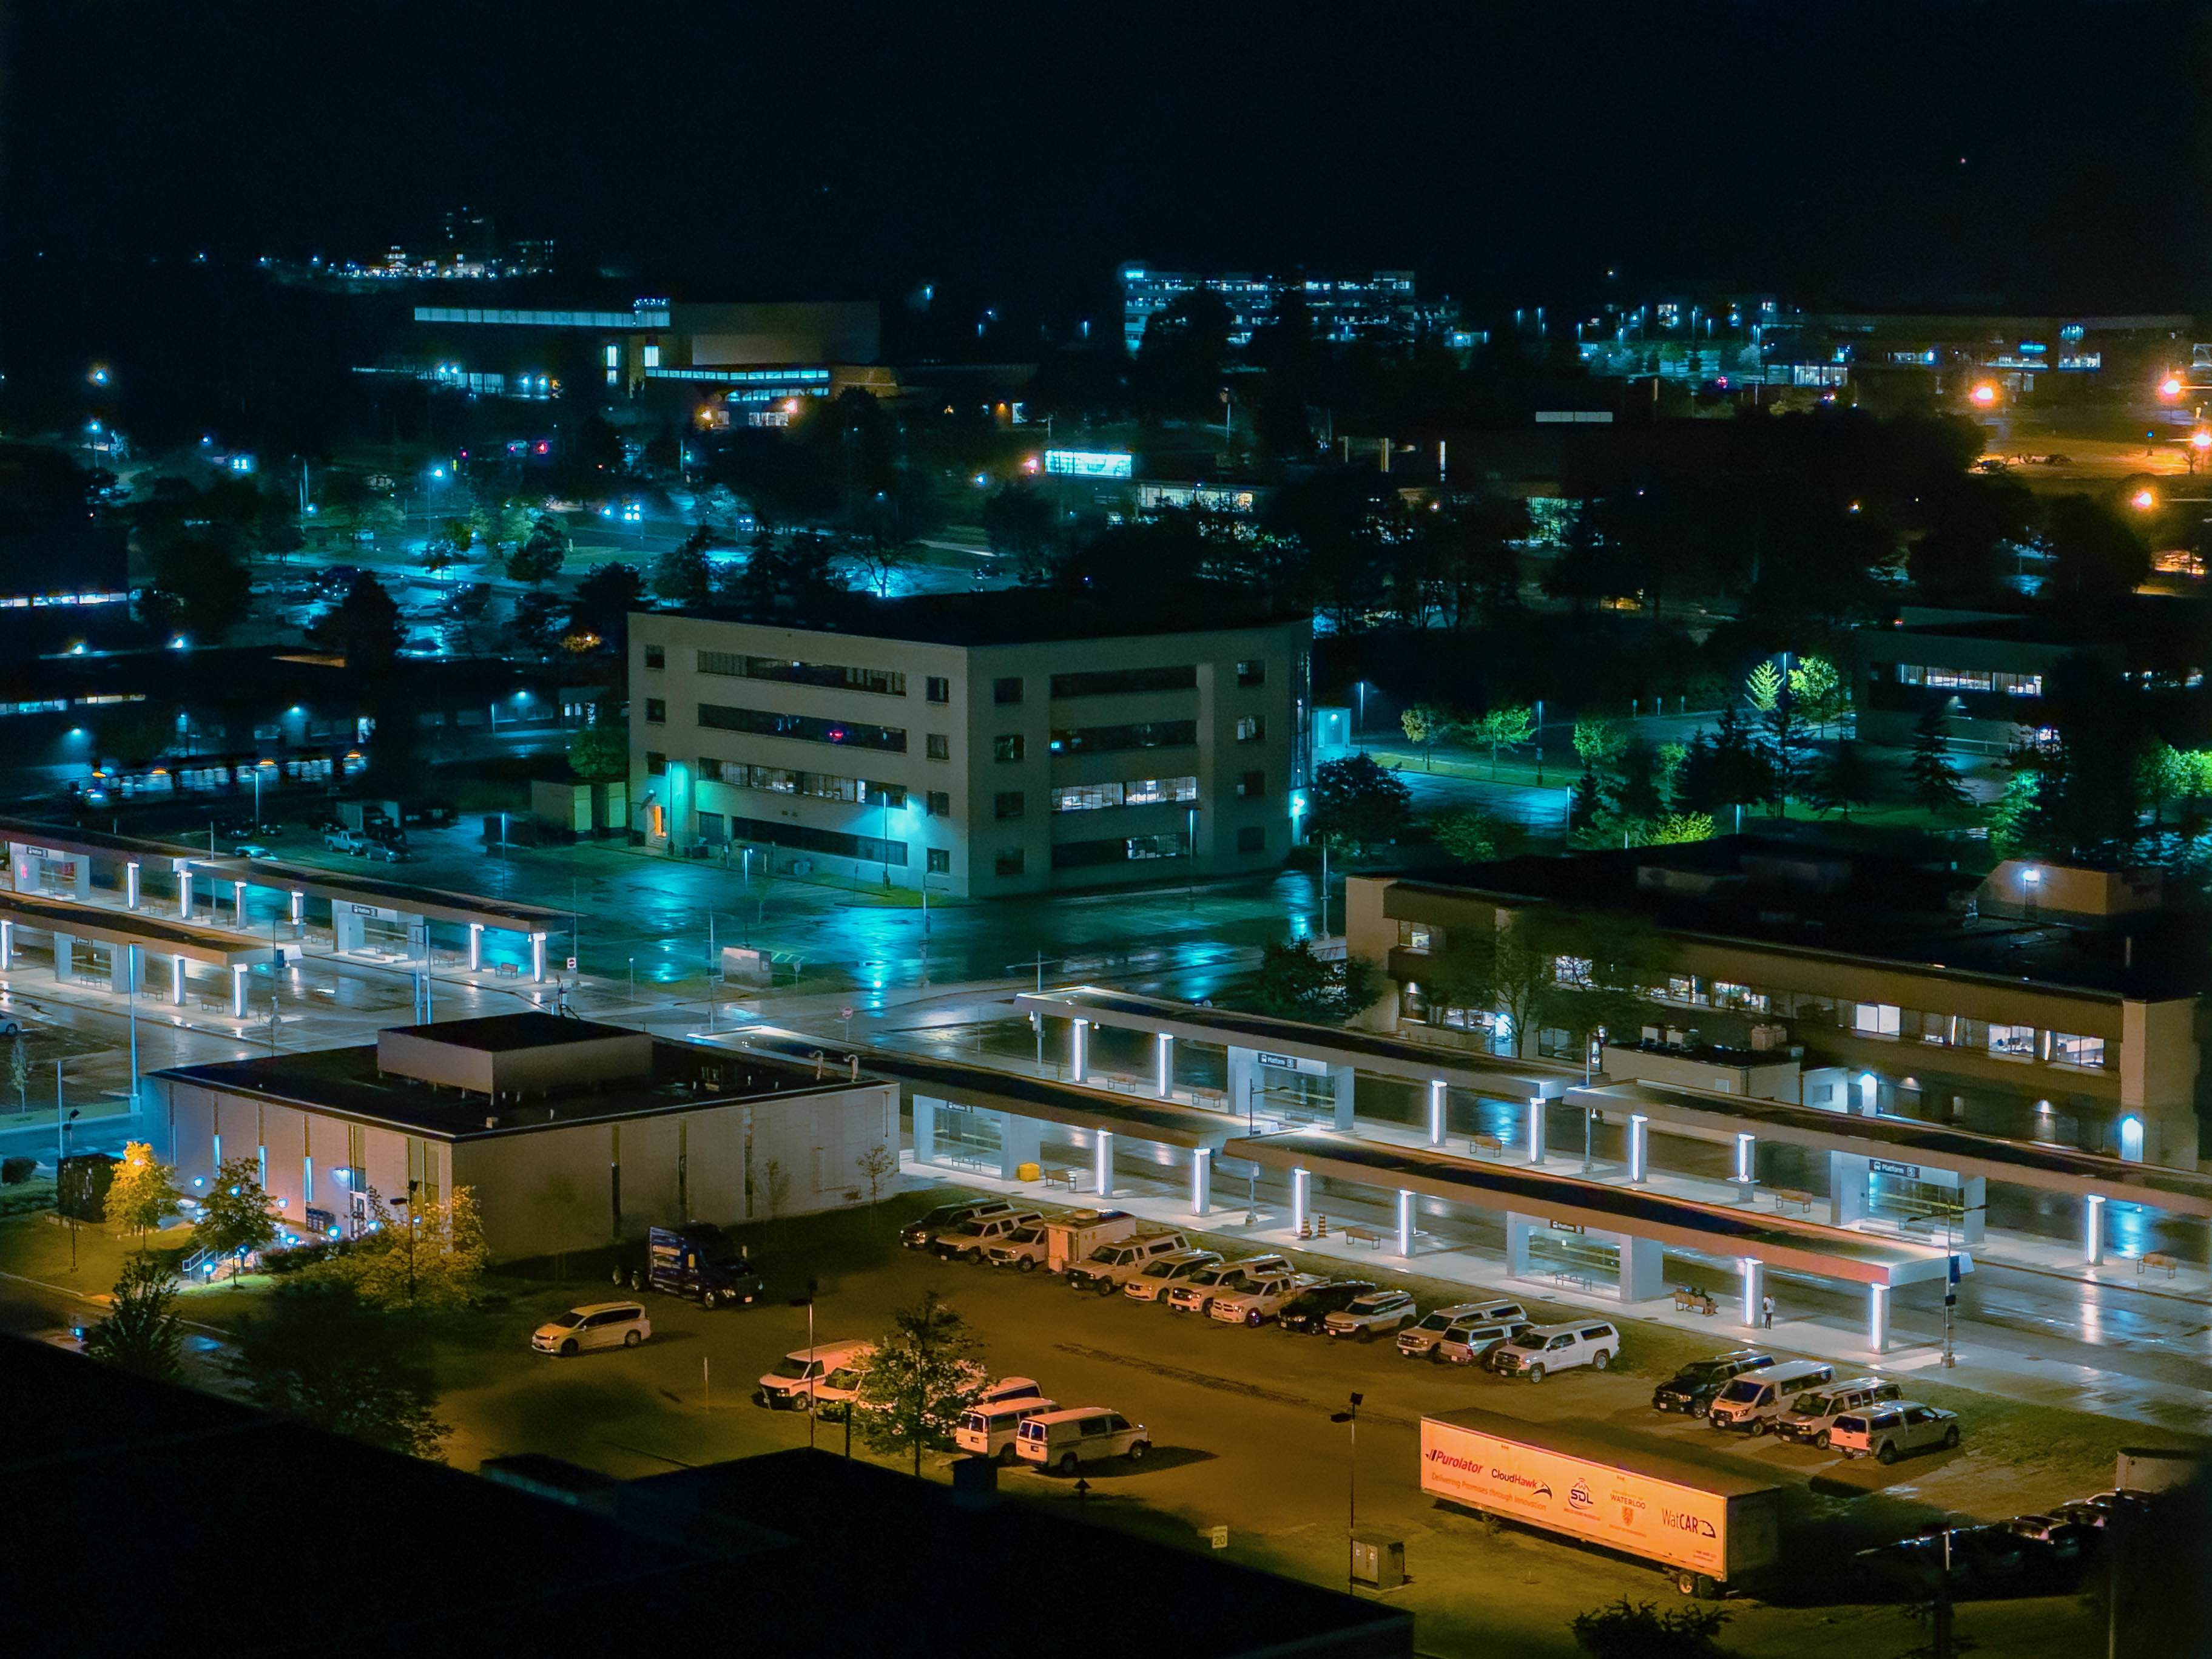
\includegraphics[scale=0.1]{img/loo.jpg}
    \caption{Waterloo, ON}
\end{figure}

\end{document}